\chapter*{Lampiran}
\begin{enumerate}
    \item Data Keseluruhan
    \begin{longtable}{|c|c|c|c|c|}
    \hline
    \textbf{Date} & \textbf{PRECTOTCORR} & \textbf{Longitude} & \textbf{Latitude} & \textbf{Wilayah} \\
    \hline
    \endfirsthead

    \hline
    \textbf{Date} & \textbf{PRECTOTCORR} & \textbf{Longitude} & \textbf{Latitude} & \textbf{Wilayah} \\
    \hline
    \endhead

    \hline
    \endfoot

    \hline
    \endlastfoot

    % ======================================================
    % ================== DATA WILAYAH TIMUR ===============
    % ======================================================
    1/31/2015  & 12.24129032 & 112.84 & -7.31 & Timur \\
    2/28/2015  & 10.2975      & 112.84 & -7.31 & Timur \\
    3/31/2015  & 8.840645161  & 112.84 & -7.31 & Timur \\
    4/30/2015  & 5.790666667  & 112.84 & -7.31 & Timur \\
    5/31/2015  & 3.477096774  & 112.84 & -7.31 & Timur \\
    6/30/2015  & 0.376        & 112.84 & -7.31 & Timur \\
    7/31/2015  & 0.15483871   & 112.84 & -7.31 & Timur \\
    8/31/2015  & 0.219032258  & 112.84 & -7.31 & Timur \\
    9/30/2015  & 0.013        & 112.84 & -7.31 & Timur \\
    10/31/2015 & 0            & 112.84 & -7.31 & Timur \\
    11/30/2015 & 2.693666667  & 112.84 & -7.31 & Timur \\
    12/31/2015 & 5.48871      & 112.84 & -7.10 & Timur \\
    \multicolumn{1}{|c|}{$\vdots$} &
    \multicolumn{1}{c|}{$\vdots$} &
    \multicolumn{1}{c|}{$\vdots$} &
    \multicolumn{1}{c|}{$\vdots$} &
    \multicolumn{1}{c|}{$\vdots$} \\
    1/31/2024  & 8.01516129   & 112.84 & -7.31 & Timur \\
    2/29/2024  & 11.49931034  & 112.84 & -7.31 & Timur \\
    3/31/2024  & 5.201612903  & 112.84 & -7.31 & Timur \\
    4/30/2024  & 7.265        & 112.84 & -7.31 & Timur \\
    5/31/2024  & 0.539067742  & 112.84 & -7.31 & Timur \\
    6/30/2024  & 1.507333333  & 112.84 & -7.31 & Timur \\
    7/31/2024  & 0.777741935  & 112.84 & -7.31 & Timur \\
    8/31/2024  & 0.029677419  & 112.84 & -7.31 & Timur \\
    9/30/2024  & 0.612666667  & 112.84 & -7.31 & Timur \\
    10/31/2024 & 1.226771494  & 112.84 & -7.31 & Timur \\
    11/30/2024 & 5.631        & 112.84 & -7.31 & Timur \\
    12/31/2024 & 12.3116129   & 112.84 & -7.31 & Timur \\
    \hline

    % ======================================================
    % ================== DATA WILAYAH BARAT ===============
    % ======================================================
    1/31/2015  & 13.95225806  & 112.61 & -7.24 & Barat \\
    2/28/2015  & 11.87321429   & 112.61 & -7.24 & Barat \\
    3/31/2015  & 9.44516129    & 112.61 & -7.24 & Barat \\
    4/30/2015  & 7.664666667   & 112.61 & -7.24 & Barat \\
    5/31/2015  & 3.707096774   & 112.61 & -7.24 & Barat \\
    6/30/2015  & 0.404         & 112.61 & -7.24 & Barat \\
    7/31/2015  & 0.044193548   & 112.61 & -7.24 & Barat \\
    8/31/2015  & 0.253225806   & 112.61 & -7.24 & Barat \\
    9/30/2015  & 0.002666667   & 112.61 & -7.24 & Barat \\
    10/31/2015 & 0.000645161   & 112.61 & -7.24 & Barat \\
    11/30/2015 & 3.233         & 112.61 & -7.24 & Barat \\
    12/31/2015 & 5.888709677   & 112.61 & -7.24 & Barat \\
    \multicolumn{1}{|c|}{$\vdots$} &
    \multicolumn{1}{c|}{$\vdots$} &
    \multicolumn{1}{c|}{$\vdots$} &
    \multicolumn{1}{c|}{$\vdots$} &
    \multicolumn{1}{c|}{$\vdots$} \\
    1/31/2024  & 9.657419355   & 112.61 & -7.24 & Barat \\
    2/29/2024  & 13.18304483   & 112.61 & -7.24 & Barat \\
    3/31/2024  & 6.666129032   & 112.61 & -7.24 & Barat \\
    4/30/2024  & 8.748666667   & 112.61 & -7.24 & Barat \\
    5/31/2024  & 0.61516129    & 112.61 & -7.24 & Barat \\
    6/30/2024  & 2.328         & 112.61 & -7.24 & Barat \\
    7/31/2024  & 0.880645161   & 112.61 & -7.24 & Barat \\
    8/31/2024  & 0.102258065   & 112.61 & -7.24 & Barat \\
    9/30/2024  & 1.314         & 112.61 & -7.24 & Barat \\
    10/31/2024 & 1.468064516   & 112.61 & -7.24 & Barat \\
    11/30/2024 & 6.292666667   & 112.61 & -7.24 & Barat \\
    12/31/2024 & 13.62387097   & 112.61 & -7.24 & Barat \\
    \hline

    % ======================================================
    % ================== DATA WILAYAH SELATAN =============
    % ======================================================
    1/31/2015  & 14.30387097 & 112.73 & -7.35 & Selatan \\
    2/28/2015  & 12.15035714 & 112.73 & -7.35 & Selatan \\
    3/31/2015  & 11.21225806 & 112.73 & -7.35 & Selatan \\
    4/30/2015  & 7.384        & 112.73 & -7.35 & Selatan \\
    5/31/2015  & 3.871935484  & 112.73 & -7.35 & Selatan \\
    6/30/2015  & 0.249333333  & 112.73 & -7.35 & Selatan \\
    7/31/2015  & 0.038064516  & 112.73 & -7.35 & Selatan \\
    8/31/2015  & 0.269354839  & 112.73 & -7.35 & Selatan \\
    9/30/2015  & 0.001666667  & 112.73 & -7.35 & Selatan \\
    10/31/2015 & 0            & 112.73 & -7.35 & Selatan \\
    11/30/2015 & 3.351666667  & 112.73 & -7.35 & Selatan \\
    12/31/2015 & 5.399354839  & 112.73 & -7.35 & Selatan \\
    \multicolumn{1}{|c|}{$\vdots$} &
    \multicolumn{1}{c|}{$\vdots$} &
    \multicolumn{1}{c|}{$\vdots$} &
    \multicolumn{1}{c|}{$\vdots$} &
    \multicolumn{1}{c|}{$\vdots$} \\
    1/31/2024  & 9.912258065  & 112.73 & -7.35 & Selatan \\
    2/29/2024  & 13.8037931   & 112.73 & -7.35 & Selatan \\
    3/31/2024  & 4.729354839  & 112.73 & -7.35 & Selatan \\
    4/30/2024  & 9.16         & 112.73 & -7.35 & Selatan \\
    5/31/2024  & 0.340645161  & 112.73 & -7.35 & Selatan \\
    6/30/2024  & 2.391        & 112.73 & -7.35 & Selatan \\
    7/31/2024  & 0.822580645  & 112.73 & -7.35 & Selatan \\
    8/31/2024  & 0.074838871  & 112.73 & -7.35 & Selatan \\
    9/30/2024  & 1.493        & 112.73 & -7.35 & Selatan \\
    10/31/2024 & 1.249032258  & 112.73 & -7.35 & Selatan \\
    11/30/2024 & 6.636666667  & 112.73 & -7.35 & Selatan \\
    12/31/2024 & 13.51903226  & 112.73 & -7.35 & Selatan \\
    \hline

    % ======================================================
    % ================== DATA WILAYAH UTARA ===============
    % ======================================================
    1/31/2015  & 13.89774194  & 112.73 & -7.2 & Utara \\
    2/28/2015  & 11.93107143  & 112.73 & -7.2 & Utara \\
    3/31/2015  & 9.387419355  & 112.73 & -7.2 & Utara \\
    4/30/2015  & 7.462333333  & 112.73 & -7.2 & Utara \\
    5/31/2015  & 3.97516129   & 112.73 & -7.2 & Utara \\
    6/30/2015  & 0.409333333  & 112.73 & -7.2 & Utara \\
    7/31/2015  & 0.040645161  & 112.73 & -7.2 & Utara \\
    8/31/2015  & 0.256129032  & 112.73 & -7.2 & Utara \\
    9/30/2015  & 0.003333333  & 112.73 & -7.2 & Utara \\
    10/31/2015 & 0.000645161  & 112.73 & -7.2 & Utara \\
    11/30/2015 & 3.227        & 112.73 & -7.2 & Utara \\
    12/31/2015 & 5.791935484  & 112.73 & -7.2 & Utara \\
    \multicolumn{1}{|c|}{$\vdots$} &
    \multicolumn{1}{c|}{$\vdots$} &
    \multicolumn{1}{c|}{$\vdots$} &
    \multicolumn{1}{c|}{$\vdots$} &
    \multicolumn{1}{c|}{$\vdots$} \\ 
    1/31/2024  & 9.479677419  & 112.73 & -7.2 & Utara \\
    2/29/2024  & 13.38482759  & 112.73 & -7.2 & Utara \\
    3/31/2024  & 6.628709677  & 112.73 & -7.2 & Utara \\
    4/30/2024  & 8.795         & 112.73 & -7.2 & Utara \\
    5/31/2024  & 0.610967742   & 112.73 & -7.2 & Utara \\
    6/30/2024  & 2.319         & 112.73 & -7.2 & Utara \\
    7/31/2024  & 0.882258065   & 112.73 & -7.2 & Utara \\
    8/31/2024  & 0.117741935   & 112.73 & -7.2 & Utara \\
    9/30/2024  & 1.306333333   & 112.73 & -7.2 & Utara \\
    10/31/2024 & 1.127096774   & 112.73 & -7.2 & Utara \\
    11/30/2024 & 6.537         & 112.73 & -7.2 & Utara \\
    12/31/2024 & 13.60354839   & 112.73 & -7.2 & Utara \\
    \hline

    % ======================================================
    % ================== DATA WILAYAH TENGAH ==============
    % ======================================================
    1/31/2015  & 14.25870968  & 112.74 & -7.26 & Tengah \\
    2/28/2015  & 12.17071429  & 112.74 & -7.26 & Tengah \\
    3/31/2015  & 11.19290323  & 112.74 & -7.26 & Tengah \\
    4/30/2015  & 7.007         & 112.74 & -7.26 & Tengah \\
    5/31/2015  & 4.287741935   & 112.74 & -7.26 & Tengah \\
    6/30/2015  & 0.249666667   & 112.74 & -7.26 & Tengah \\
    7/31/2015  & 0.038837097   & 112.74 & -7.26 & Tengah \\
    8/31/2015  & 0.269677419   & 112.74 & -7.26 & Tengah \\
    9/30/2015  & 0.001666667   & 112.74 & -7.26 & Tengah \\
    10/31/2015 & 0             & 112.74 & -7.26 & Tengah \\
    11/30/2015 & 3.352666667   & 112.74 & -7.26 & Tengah \\
    12/31/2015 & 5.317741935   & 112.74 & -7.26 & Tengah \\
    \multicolumn{1}{|c|}{$\vdots$} &
    \multicolumn{1}{c|}{$\vdots$} &
    \multicolumn{1}{c|}{$\vdots$} &
    \multicolumn{1}{c|}{$\vdots$} &
    \multicolumn{1}{c|}{$\vdots$} \\
    1/31/2024  & 9.722258065   & 112.74 & -7.26 & Tengah \\
    2/29/2024  & 14.05206897   & 112.74 & -7.26 & Tengah \\
    3/31/2024  & 4.01290323    & 112.74 & -7.26 & Tengah \\
    4/30/2024  & 9.200666667   & 112.74 & -7.26 & Tengah \\
    5/31/2024  & 0.341935484   & 112.74 & -7.26 & Tengah \\
    6/30/2024  & 2.375         & 112.74 & -7.26 & Tengah \\
    7/31/2024  & 0.830322581   & 112.74 & -7.26 & Tengah \\
    8/31/2024  & 0.083548387   & 112.74 & -7.26 & Tengah \\
    9/30/2024  & 1.493         & 112.74 & -7.26 & Tengah \\
    10/31/2024 & 0.837096774   & 112.74 & -7.26 & Tengah \\
    11/30/2024 & 6.660666667   & 112.74 & -7.26 & Tengah \\
    12/31/2024 & 13.59290323   & 112.74 & -7.26 & Tengah \\

\end{longtable}

    \item Data Train
    \begin{longtable}{|c|c|c|c|c|}

    \hline
    \textbf{Barat} & \textbf{Selatan} & \textbf{Tengah} & \textbf{Timur} & \textbf{Utara} \\
    \hline
    \endfirsthead

    \hline
    \textbf{Barat} & \textbf{Selatan} & \textbf{Tengah} & \textbf{Timur} & \textbf{Utara} \\
    \hline
    \endhead

    \hline
    \endfoot

    \hline
    \endlastfoot

    % ===========================
    % ====== ISI DATA DI SINI ===
    % ===========================
    13.9522581 & 14.303871 & 14.258710 & 12.241903 & 13.8977419 \\ \hline
    11.8732143 & 12.150357 & 12.170714 & 10.297500 & 11.9310714 \\ \hline
    9.4451613  & 11.212258 & 11.192903 & 8.8406452 & 9.3874194  \\ \hline
    7.6646667  & 7.384000  & 7.007000  & 5.7906667 & 7.4623333  \\ \hline
    3.7070968  & 3.871935  & 4.287742  & 3.4770968 & 3.9751613  \\ \hline
    0.4040000  & 0.249333  & 0.249667  & 0.3760000 & 0.4093333  \\ \hline
    0.0441935  & 0.038065  & 0.038387  & 0.0154839 & 0.0406452  \\ \hline
    0.2532258  & 0.269355  & 0.269677  & 0.2190323 & 0.2561290  \\ \hline
    0.0026667  & 0.0017    & 0.0016667 & 0.0130000 & 0.0033333  \\ \hline
    % Checkpoint
    0.0006452 & 0 & 0 & 0 & 0.0000452 \\ \hline
    3.2330000 & 3.351667 & 3.352667 & 2.6936667 & 5.7918355 \\ \hline
    5.8887097 & 5.399355 & 5.317742 & 5.6648387 & 17.7812903 \\ \hline
    7.6958065 & 7.416774 & 7.486774 & 6.9264516 & 16.2137903 \\ \hline
    16.2608968 & 16.252607 & 16.232759 & 12.477016 & 40.6182258 \\ \hline
    6.0390323 & 6.234516 & 6.254839 & 5.6167742 & 7.2476667 \\ \hline
    7.4933333 & 7.335333 & 7.246467 & 7.0996667 & 8.8454839 \\ \hline
    8.7500000 & 9.826129 & 9.908710 & 9.4874194 & 4.8880000 \\ \hline
    4.9133333 & 4.612333 & 4.607000 & 4.6306774 & 4.4390323 \\ \hline
    4.4196774 & 4.740645 & 4.745161 & 4.3209677 & 2.1390323 \\ \hline
    2.3100000 & 2.354516 & 2.355161 & 1.9212903 & 2.1435484 \\ \hline
    4.5103333 & 4.512000 & 4.460333 & 2.9830000 & 4.4476667 \\ \hline
    8.6964516 & 9.065161 & 9.115484 & 7.4983333 & 8.7532258 \\ \hline
    5.3376667 & 5.466000 & 5.443667 & 4.4323333 & 5.3040000 \\ \hline
    10.3970968 & 9.911613 & 9.783548 & 9.0038710 & 10.1619355 \\ \hline
    13.1619355 & 13.314839 & 13.462903 & 12.5758065 & 13.4058065 \\ \hline
    9.9450000 & 9.688214 & 9.641071 & 9.4150000 & 9.8985714 \\ \hline
    6.9183871 & 6.891290 & 6.886452 & 6.7719355 & 6.9277419 \\ \hline
    6.8566667 & 7.246667 & 7.234333 & 5.7630000 & 8.6170000 \\ \hline
    4.0541935 & 3.680323 & 3.744839 & 3.7790323 & 4.1216129 \\ \hline
    2.9860000 & 2.887333 & 2.901333 & 3.4906667 & 3.0146667 \\ \hline
    1.0255806 & 1.072903 & 1.072903 & 1.1074194 & 1.0577419 \\ \hline
    0.0145161 & 0.019677 & 0.019677 & 0.1312903 & 0.0190323 \\ \hline
    0.4850000 & 0.376333 & 0.359667 & 0.2133333 & 0.4490000 \\ \hline
    2.7874194 & 2.475484 & 2.429258 & 1.4987097 & 2.8235484 \\ \hline
    9.8060000 & 9.349333 & 9.329000 & 9.6909333 & 9.7676667 \\ \hline
    11.1319355 & 10.706452 & 10.715161 & 9.8096774 & 11.1403226 \\ \hline
    9.0793548 & 8.859355 & 8.705806 & 10.7912903 & 7.1409677 \\ \hline
    14.0025000 & 15.132143 & 15.233571 & 10.5642857 & 14.0453571 \\ \hline
    9.1022903 & 9.930000 & 9.933871 & 7.9183871 & 10.2858065 \\ \hline
    4.3100000 & 4.352000 & 4.424667 & 3.1780000 & 4.3850000 \\ \hline
    4.0970968 & 4.262258 & 4.262903 & 2.6509677 & 4.2193226 \\ \hline
    2.0626667 & 2.401333 & 2.401667 & 1.5463333 & 2.0676667 \\ \hline
    0.0293548 & 0.030645 & 0.030645 & 0.0190000 & 0.0303226 \\ \hline
    0.5587097 & 0.634194 & 0.634194 & 0.7261290 & 0.5432258 \\ \hline
    0.1590000 & 0.041333 & 0.041333 & 0.0336667 & 0.1736667 \\ \hline
    0.9377097 & 0.738271 & 0.808667 & 0.3077419 & 0.2978710 \\ \hline
    5.4080000 & 5.532667 & 5.811333 & 5.4786667 & 5.5660000 \\ \hline
    9.6355484 & 10.240516 & 11.021613 & 7.5906774 & 9.2960000 \\ \hline
    15.0722581 & 14.639355 & 14.610000 & 12.7341935 & 14.0992258 \\ \hline
    17.2406935 & 18.067786 & 13.547500 & 13.4639286 & 12.2650000 \\ \hline
    8.4096774 & 7.850323 & 7.807742 & 7.3274194 & 8.8325806 \\ \hline
    8.6616667 & 9.671333 & 9.573333 & 8.5500000 & 8.4970000 \\ \hline
    0.9851613 & 0.871290 & 1.097419 & 0.4906452 & 1.2558065 \\ \hline
    % Checkpoint
    0.1136667 & 0.0500000 & 0.0500000 & 0.0526667 & 0.1136667 \\ \hline
    0.0341935 & 0.0300000 & 0.0296777 & 0.0333871 & 0.0341935 \\ \hline
    0.3422581 & 0.504516 & 0.404194 & 0.3035484 & 0.3093548 \\ \hline
    0.4550000 & 0.624667 & 0.571000 & 0.3790000 & 0.4340000 \\ \hline
    0.0522581 & 0.011613 & 0.157742 & 0.0451935 & 0.0707419 \\ \hline
    0.8136667 & 0.786000 & 0.789667 & 0.6576667 & 0.8170000 \\ \hline
    5.8129032 & 5.629355 & 5.580645 & 4.6741935 & 5.7177097 \\ \hline
    11.4467742 & 10.878387 & 10.314194 & 9.5616129 & 11.1383871 \\ \hline
    14.6462097 & 14.437931 & 15.086977 & 13.7755157 & 15.0072581 \\ \hline
    9.1287097 & 10.100323 & 10.093871 & 9.6906452 & 9.1793548 \\ \hline
    10.9736667 & 11.347667 & 11.360333 & 9.6100000 & 12.3061290 \\ \hline
    6.9148387 & 7.669032 & 7.617742 & 6.2925806 & 6.8587097 \\ \hline
    1.5520000 & 1.171000 & 1.225667 & 1.0213333 & 1.6150000 \\ \hline
    0.8629032 & 0.695161 & 0.695161 & 0.8467742 & 0.8651613 \\ \hline
    0.8274194 & 0.822581 & 0.822258 & 0.6532903 & 0.8270968 \\ \hline
    0.4460000 & 0.319000 & 0.319333 & 0.2993333 & 0.4426667 \\ \hline
    3.2245161 & 3.501935 & 3.347742 & 3.9208365 & 3.1032581 \\ \hline
    4.2633333 & 4.553333 & 4.712000 & 5.1683333 & 4.3853333 \\ \hline
    17.4945161 & 18.056774 & 17.578710 & 15.5209032 & 17.8980323 \\ \hline
    14.9816129 & 14.581290 & 14.956129 & 12.6345161 & 15.2096774 \\ \hline
    16.9085714 & 17.914643 & 17.983571 & 15.6323143 & 16.9203143 \\ \hline
    10.6554839 & 10.404516 & 10.256774 & 8.720323 & 10.5732258 \\ \hline
    3.2076667 & 3.191000 & 3.383667 & 3.440333 & 3.3916667 \\ \hline
    12.1080645 & 11.808065 & 1.807097 & 2.3787097 & 2.1209032 \\ \hline
    4.1400000 & 4.543000 & 4.541000 & 4.099667 & 4.1476667 \\ \hline
    0.2703226 & 0.302258 & 0.303023 & 0.3738710 & 0.2683548 \\ \hline
    0.3832258 & 0.284194 & 0.289032 & 0.2258065 & 0.3893548 \\ \hline
    0.2680000 & 2.434677 & 2.419000 & 2.2376667 & 2.6790000 \\ \hline
    1.9503226 & 1.184839 & 1.158387 & 1.1535484 & 1.9329032 \\ \hline
    9.9246667 & 10.540667 & 10.296767 & 10.0633333 & 9.7332000 \\ \hline
    13.2767742 & 13.717419 & 13.797097 & 13.3867742 & 13.2800000 \\ \hline
    9.9790323 & 10.203323 & 10.363548 & 9.7714935 & 10.1479032 \\ \hline
    12.2182143 & 11.081786 & 10.096071 & 11.243926 & 12.1326143 \\ \hline
    10.1454839 & 11.110000 & 11.201290 & 9.9209677 & 10.2306452 \\ \hline
    5.3926667 & 5.479333 & 5.458000 & 4.5153333 & 5.3733333 \\ \hline
    7.5806452 & 8.720645 & 8.635806 & 7.1425806 & 7.552806 \\ \hline
    4.5080000 & 4.860333 & 4.990667 & 3.9916667 & 5.1663333 \\ \hline
    2.7145161 & 2.675484 & 2.675806 & 1.8054839 & 2.7409677 \\ \hline
    0.7350000 & 0.731444 & 0.741000 & 0.6045161 & 0.8190000 \\ \hline
    2.4716667 & 2.898333 & 2.826333 & 2.0676667 & 2.3710000 \\ \hline
    2.7483871 & 2.928774 & 2.893871 & 2.1570968 & 3.7022581 \\ \hline
    9.3650000 & 9.823333 & 9.300000 & 9.9753333 & 9.4416667 \\ \hline
    9.13577419 & 17.739355 & 7.490645 & 6.8522581 & 8.79703226 \\ \hline
    9.5374194 & 9.942581 & 10.157742 & 7.9122581 & 9.8416129 \\ \hline
    % Chackpoint
    16.8142857 & 17.490714 & 17.365714 & 14.3935714 & 16.7035714 \\ \hline
    6.7612903  & 6.586452  & 6.588710  & 6.4235484  & 6.8174194  \\ \hline
    8.4820000  & 9.307667  & 9.474333  & 7.2303333  & 8.5806667  \\ \hline
    2.1967742  & 1.957742  & 1.965806  & 1.4864516  & 2.2161290  \\ \hline
    0.5126667  & 0.401000  & 0.400333  & 0.5450000  & 0.5096667  \\ \hline
    2.3080645  & 1.745484  & 1.746774  & 2.0241935  & 2.3116129  \\ \hline
    0.0780645  & 0.052903  & 0.052903  & 0.0667742  & 0.0783871  \\ \hline
    0.0443333  & 0.031000  & 0.031000  & 0.0646667  & 0.0443333  \\ \hline
    0.0735484  & 0.054516  & 0.054194  & 0.0096774  & 0.0719355  \\ \hline
    3.5803333  & 2.410000  & 2.394000  & 2.7973333  & 3.4723333  \\ \hline
    24.714193  & 28.639355 & 28.602903 & 16.1096774 & 24.7951613 \\ \hline
\end{longtable}

    \item Data Test
    \begin{longtable}{|c|c|c|c|c|}

    \hline
    \textbf{Barat} & \textbf{Selatan} & \textbf{Tengah} & \textbf{Timur} & \textbf{Utara} \\
    \hline
    \endfirsthead

    \hline
    \textbf{Barat} & \textbf{Selatan} & \textbf{Tengah} & \textbf{Timur} & \textbf{Utara} \\
    \hline
    \endhead

    \hline
    \endfoot

    \hline
    \endlastfoot

    % ===========================
    % ====== ISI DATA DI SINI ===
    % ===========================
    9.6574   & 9.91226  & 9.72226  & 8.01516  & 9.4797  \\ \hline
    13.1803  & 13.80379 & 14.05207 & 11.49931 & 13.3848 \\ \hline
    6.6661   & 4.72935  & 4.70129  & 5.20161  & 6.6287  \\ \hline
    8.7487   & 9.16000  & 9.20067  & 7.26500  & 8.7950  \\ \hline
    0.6152   & 0.34065  & 0.34194  & 0.53907  & 0.6110  \\ \hline
    2.3280   & 2.39100  & 2.37500  & 1.50733  & 2.3190  \\ \hline
    0.8806   & 0.82258  & 0.83032  & 0.77774  & 0.8823  \\ \hline
    0.1023   & 0.07484  & 0.08355  & 0.02968  & 0.1177  \\ \hline
    1.3140   & 1.49300  & 1.49300  & 0.61267  & 1.3063  \\ \hline
    1.4681   & 1.24903  & 0.83710  & 1.22677  & 1.1271  \\ \hline
    6.2927   & 6.36367  & 6.66067  & 5.63100  & 6.5370  \\ \hline
    13.6139  & 13.51903 & 13.59290 & 12.31161 & 13.6035 \\ \hline
\end{longtable}

    \item ARIMA Plot ACF dan PACF
    \begin{enumerate}[label=\alph*.]
    \item Plot ACF dan PACF sebelum Transformasi
    \begin{enumerate}[label=\roman*.]
        \item Barat
            \begin{figure}[H]
                \centering
                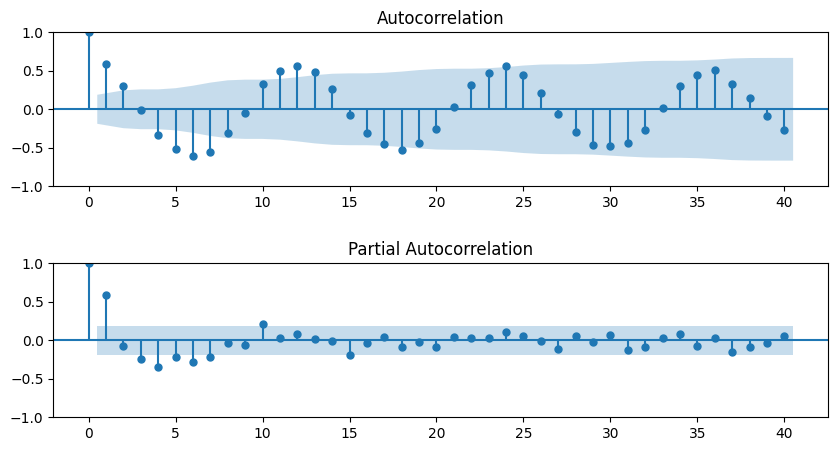
\includegraphics[width=0.9\textwidth]{images/lampiran/ARIMA-ACF-PACF-BARAT-SEBELUM.png}
            \end{figure}
        \item Selatan
            \begin{figure}[H]
                \centering
                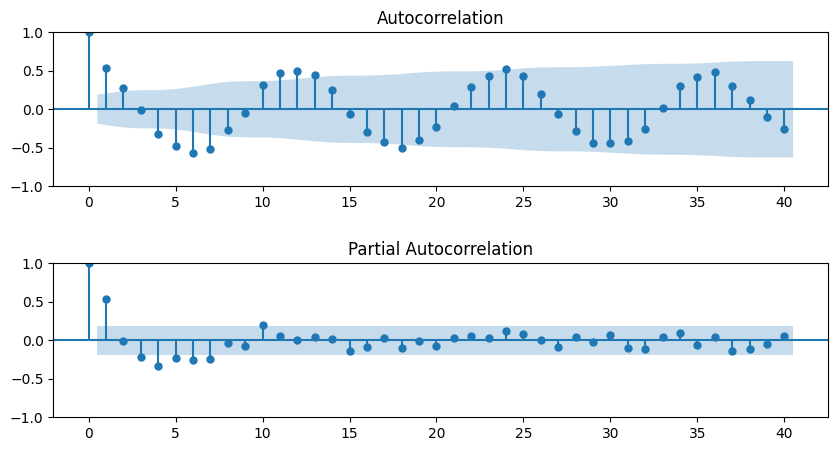
\includegraphics[width=0.9\textwidth]{images/lampiran/ARIMA-ACF-PACF-SELATAN-SEBELUM.png}
            \end{figure}
        \item Tengah
            \begin{figure}[H]
                \centering
                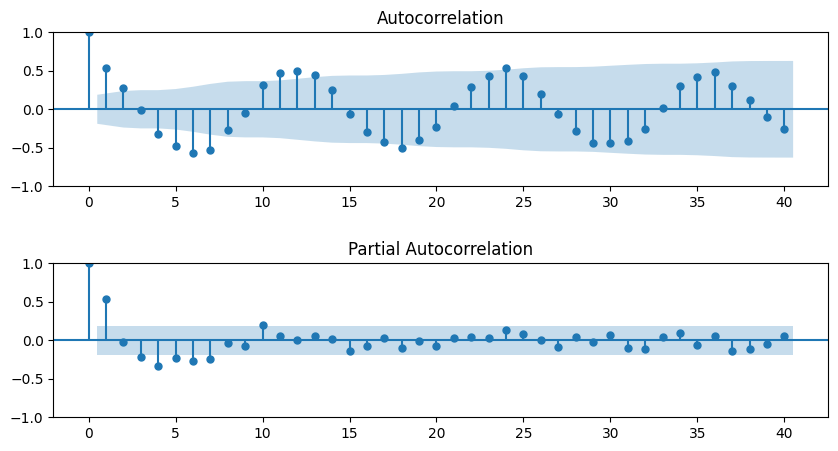
\includegraphics[width=0.9\textwidth]{images/lampiran/ARIMA-ACF-PACF-TENGAH-SEBELUM.png}
            \end{figure}
        \item Timur
            \begin{figure}[H]
                \centering
                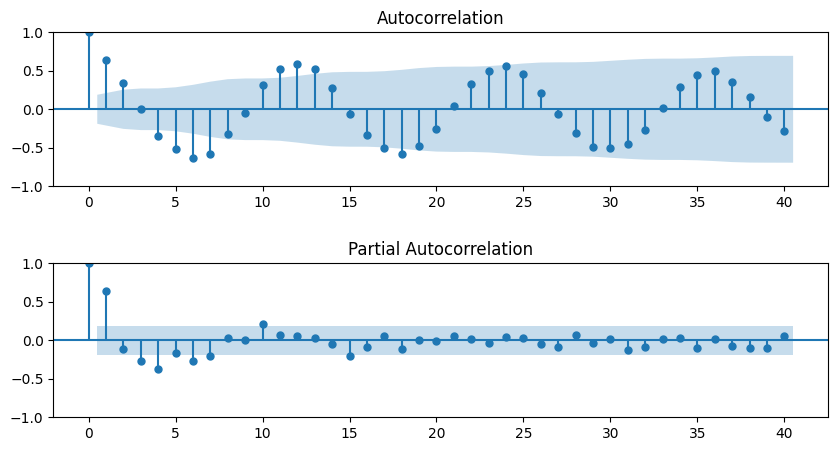
\includegraphics[width=0.9\textwidth]{images/lampiran/ARIMA-ACF-PACF-TIMUR-SEBELUM.png}
            \end{figure}
        \item Utara
            \begin{figure}[H]
                \centering
                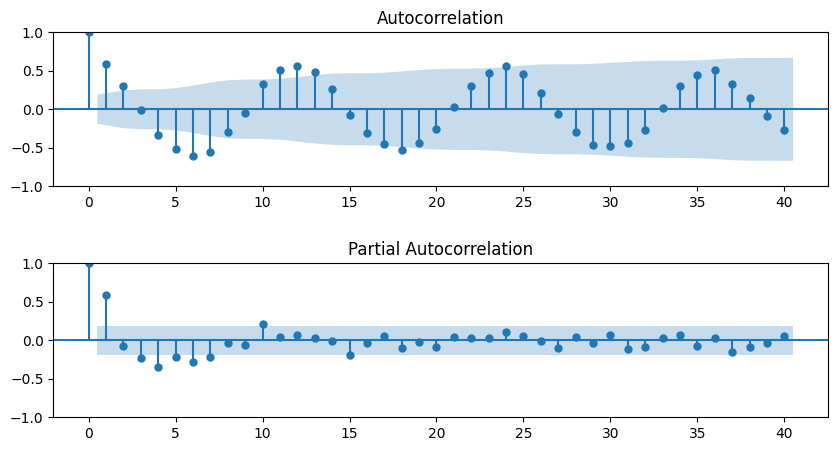
\includegraphics[width=0.9\textwidth]{images/lampiran/ARIMA-ACF-PACF-UTARA-SEBELUM.png}
            \end{figure}
    \end{enumerate}
    \item Plot ACF dan PACF setelah Transformasi
    \begin{enumerate}[label=\roman*.]
        \item Barat
            \begin{figure}[H]
                \centering
                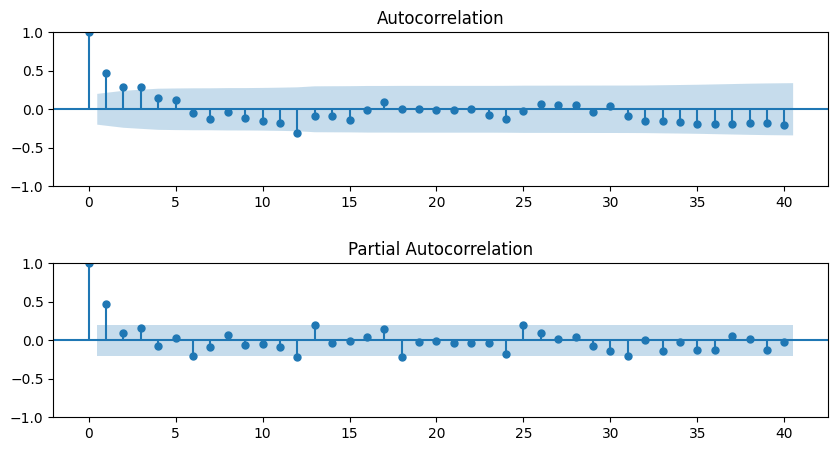
\includegraphics[width=0.9\textwidth]{images/lampiran/ARIMA-ACF-PACF-BARAT-SETELAH.png}
            \end{figure}
        \item Selatan
            \begin{figure}[H]
                \centering
                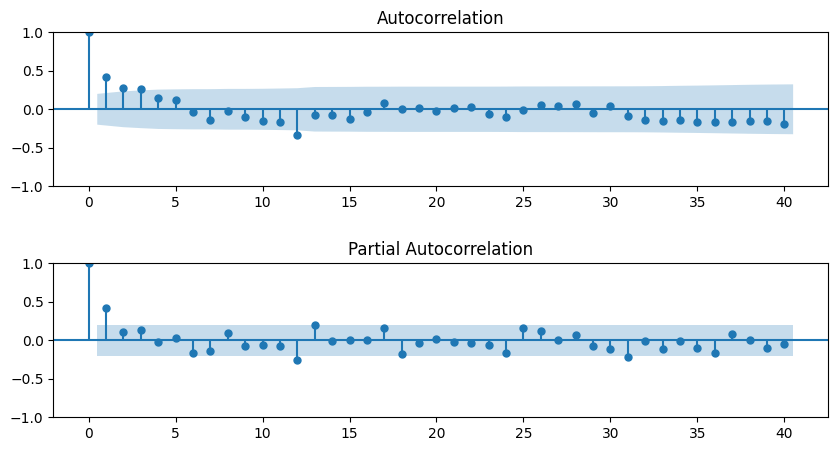
\includegraphics[width=0.9\textwidth]{images/lampiran/ARIMA-ACF-PACF-SELATAN-SETELAH.png}
            \end{figure}
        \item Tengah
            \begin{figure}[H]
                \centering
                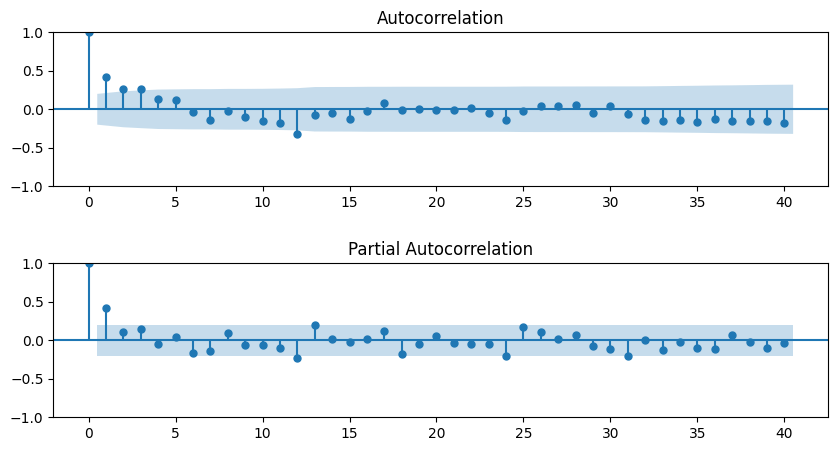
\includegraphics[width=0.9\textwidth]{images/lampiran/ARIMA-ACF-PACF-TENGAH-SETELAH.png}
            \end{figure}
        \item Timur
            \begin{figure}[H]
                \centering
                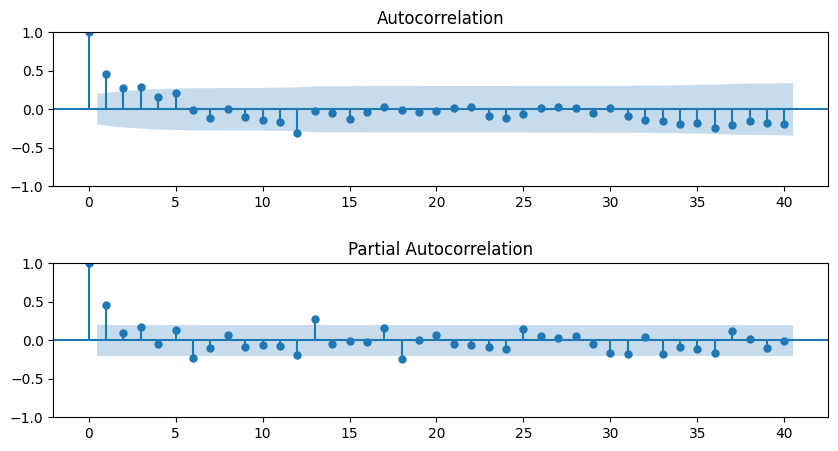
\includegraphics[width=0.9\textwidth]{images/lampiran/ARIMA-ACF-PACF-TIMUR-SETELAH.png}
            \end{figure}
        \item Utara
            \begin{figure}[H]
                \centering
                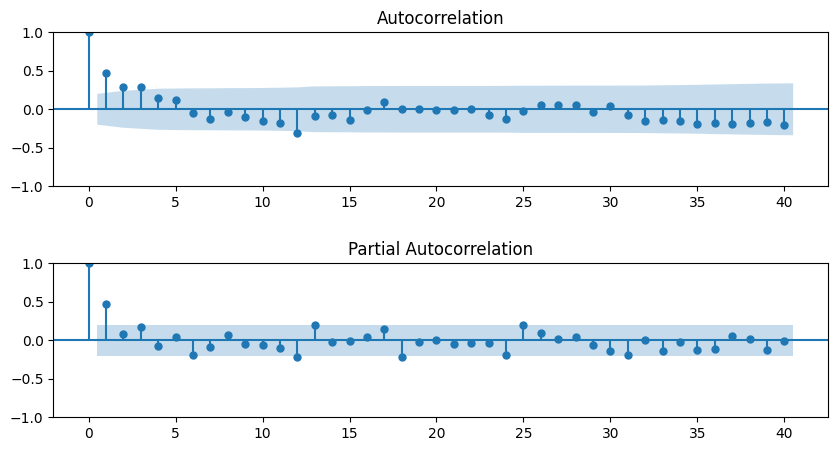
\includegraphics[width=0.9\textwidth]{images/lampiran/ARIMA-ACF-PACF-UTARA-SETELAH.png}
            \end{figure}
    \end{enumerate}
\end{enumerate}

    \item ARIMA Estimasi Parameter Barat
    \tiny
\begin{longtable}{|c|c|c|c|c|c|c|c|c|}
    \hline
    \multirow{3}{*}{\textbf{Model}} &
    \multirow{3}{*}{\textbf{Statistik}} &
    \multicolumn{3}{c|}{\textbf{AR Parameter}} &
    \multicolumn{3}{c|}{\textbf{MA Parameter}} &
    \multirow{3}{*}{\textbf{RMSE}} \\ 
    \cline{3-8}

    & & 
    \multicolumn{2}{c|}{\textbf{Non Seasonal}} &
    \textbf{Seasonal} &
    \multicolumn{2}{c|}{\textbf{Non Seasonal}} &
    \textbf{Seasonal} &
    \\
    \cline{3-8}

    & & 
    \textbf{AR1} & \textbf{AR2} & \textbf{AR} &
    \textbf{MA1} & \textbf{MA2} & \textbf{MA} &
    \\
    \hline
    \endfirsthead

    % =================== HEADER REPEAT =====================
    \hline
    \multirow{3}{*}{\textbf{Model}} &
    \multirow{3}{*}{\textbf{Statistik}} &
    \multicolumn{3}{c|}{\textbf{AR Parameter}} &
    \multicolumn{3}{c|}{\textbf{MA Parameter}} &
    \multirow{3}{*}{\textbf{RMSE}} \\ 
    \cline{3-8}

    & & 
    \multicolumn{2}{c|}{\textbf{Non Seasonal}} &
    \textbf{Seasonal} &
    \multicolumn{2}{c|}{\textbf{Non Seasonal}} &
    \textbf{Seasonal} &
    \\
    \cline{3-8}

    & & 
    \textbf{AR1} & \textbf{AR2} & \textbf{AR} &
    \textbf{MA1} & \textbf{MA2} & \textbf{MA} &
    \\
    \hline
    \endhead

    \hline
    \endfoot

    \hline
    \endlastfoot

    % ===========================
    % ====== ISI DATA DI SINI ===
    % ===========================

    % ===================== MODEL 1 ======================
    \multirow{4}{*}{\centering (0,1,0) × (0,1,0)\textsubscript{12}} 
    & Estimasi &  &  &  &  &  &  & 
    \multirow{4}{*}{\centering 5.156} \\ \cline{2-8}

    & SE       &  &  &  &  &  &  &  \\ \cline{2-8}

    & t-value  &  &  &  &  &  &  &  \\ \cline{2-8}

    & p-value  &  &  &  &  &  &  &  \\ \hline

    % ===================== MODEL 2 ======================
    \multirow{4}{*}{\centering (0,1,0) × (0,1,1)\textsubscript{12}} 
    & Estimasi &  &  &  &  &  & -1.0000 & 
    \multirow{4}{*}{\centering 4.944} \\ \cline{2-8}

    & SE       &  &  &  &  &  & 1.54e+04 &  \\ \cline{2-8}

    & t-value  &  &  &  &  &  & -6.5e-0 &  \\ \cline{2-8}

    & p-value  &  &  &  &  &  & 1.000 &  \\ \hline

    % ===================== MODEL 3 ======================
    \multirow{4}{*}{\centering (0,1,0) × (1,1,0)\textsubscript{12}}
    & Estimasi &  &  & -0.5332 &  &  &  & 
    \multirow{4}{*}{\centering 6.224} \\ \cline{2-8}

    & SE       &  &  & 0.117 &  &  &  &  \\ \cline{2-8}

    & t-value  &  &  & -4.552 &  &  &  &  \\ \cline{2-8}

    & p-value  &  &  & 0.000 &  &  &  &  \\ \hline

    % ===================== MODEL 4 ======================
    \multirow{4}{*}{\centering (0,1,1) × (1,1,1)\textsubscript{12}}
    & Estimasi &  &  & -0.3972 &  &  & -1.0000 & 
    \multirow{4}{*}{\centering 6.216} \\ \cline{2-8}

    & SE       &  &  & 0.175 &  &  & 3947.041 &  \\ \cline{2-8}

    & t-value  &  &  & -2.273 &  &  & -0.000 &  \\ \cline{2-8}

    & p-value  &  &  & 0.023 &   &  & 1.000 &  \\ \hline

    % ===================== MODEL 5 ======================
    \multirow{4}{*}{\centering (0,1,1) × (0,1,1)\textsubscript{12}}
    & Estimasi &  &  &  & -0.7275 &  & -1.0000 &
    \multirow{4}{*}{\centering 7.046} \\ \cline{2-8}

    & SE       & &  &  & 0.078  &  & 4878.768 & \\ \cline{2-8}

    & t-value  &  &  & & -9.333 &  & -0.000 & \\ \cline{2-8}

    & p-value  & &  &  & 0.000  &  & 1.000  & \\ \hline

    % ===================== MODEL 6 ======================
    \multirow{4}{*}{\centering (0,1,1) × (1,1,0)\textsubscript{12}}
    & Estimasi &  &  & -0.4895 & -1.2368 &  &  &
    \multirow{4}{*}{\centering 6.975} \\ \cline{2-8}

    & SE       &  &  & 0.106  & 0.102  &  &  & \\ \cline{2-8}

    & t-value  &  &  & -4.636 & -12.782 &  &  & \\ \cline{2-8}

    & p-value  &  &  & 0.000  & 0.000 &  &  & \\ \hline

    % ===================== MODEL 7 ======================
    \multirow{4}{*}{\centering (0,1,1) × (1,1,1)\textsubscript{12}}
    & Estimasi &   &  & -0.3644 & -0.7686 &  & -1.0000 &
    \multirow{4}{*}{\centering 6.948} \\ \cline{2-8}

    & SE       &  &  & 0.144  & 0.076 &  & 3443.042 & \\ \cline{2-8}

    & t-value  &  &  & -2.539 & -10.081 &  & -0.000 & \\ \cline{2-8}

    & p-value  &  &  & 0.011  & 0.000 &  & 1.000 & \\ \hline

    % ===================== MODEL 8 ======================
    \multirow{4}{*}{\centering (1,1,0) × (0,1,0)\textsubscript{12}}
    & Estimasi & -0.3800 &  &  &  &  &  &
    \multirow{4}{*}{\centering 3.332} \\ \cline{2-8}

    & SE       & 0.112 &   &  &  &  &  & \\ \cline{2-8}

    & t-value  & -3.403 &  &  &  &  &  & \\ \cline{2-8}

    & p-value  & 0.001 &   &  &  &  &  & \\ \hline

    % ===================== MODEL 9 ======================
    \multirow{4}{*}{\centering (1,1,0) × (0,1,1)\textsubscript{12}}
    & Estimasi & -0.3125 &  &  &  &  & -1.0000 &
    \multirow{4}{*}{\centering 5.112} \\ \cline{2-8}

    & SE       & 0.124 &   &  &  &  & 6145.704 & \\ \cline{2-8}

    & t-value  & -2.518 &  &  &  &  & -0.000 & \\ \cline{2-8}

    & p-value  & 0.012 &   &  &  &  & 1.000 & \\ \hline

    % ===================== MODEL 10 ======================
    \multirow{4}{*}{\centering (1,1,0) × (1,1,0)\textsubscript{12}}
    & Estimasi & -0.3169 &  & -0.4766 &  &  &  &
    \multirow{4}{*}{\centering 4.541} \\ \cline{2-8}

    & SE       & 0.138 &  & 0.123  &  &  &  & \\ \cline{2-8}

    & t-value  & -2.293 &  & 3.875  &  &  &  & \\ \cline{2-8}

    & p-value  & 0.022 &   & 0.000  &  &  &  & \\ \hline

    % ===================== MODEL 11 ======================
    \multirow{4}{*}{\centering (1,1,0) × (1,1,1)\textsubscript{12}}
    & Estimasi & -0.2868 &  & -0.3636 & &  &  -1.0000 &
    \multirow{4}{*}{\centering 5.929} \\ \cline{2-8}

    & SE       & 0.137 &   & 0.180  &  &  & 4266.697 & \\ \cline{2-8}

    & t-value  & -2.090  &  & -2.023 &  &  & -0.000 & \\ \cline{2-8}

    & p-value  & 0.037 &   & 0.043  &  &  & 1.000 & \\ \hline

    % ===================== MODEL 12 ======================
    \multirow{4}{*}{\centering (1,1,1) × (0,1,0)\textsubscript{12}}
    & Estimasi & 0.4495 &  &  & -1.0000 &  &  &
    \multirow{4}{*}{\centering 5.367} \\ \cline{2-8}

    & SE       & 0.122 &   &  & 1715.064 &  &  & \\ \cline{2-8}

    & t-value  & 3.683 &   &  & -0.001 &  &  & \\ \cline{2-8}

    & p-value  & 0.000  &  &  & 1.000 &  &  & \\ \hline

    % ===================== MODEL 13 ======================
    \multirow{4}{*}{\centering (1,1,1) × (0,1,1)\textsubscript{12}}
    & Estimasi & 0.2448 &  &  & -0.8374 &  & -1.0000 &
    \multirow{4}{*}{\centering 6.908} \\ \cline{2-8}

    & SE       & 0.173 &   &  & 0.078 & & 5342.151 &\\ \cline{2-8}

    & t-value  & 1.417  &  &  & -10.734 & & -0.000 & \\ \cline{2-8}

    & p-value  & 0.157 &   &  & 0.000  &  & 1.000 & \\ \hline

    % ===================== MODEL 14 ======================
    \multirow{4}{*}{\centering (1,1,1) × (1,1,0)\textsubscript{12}}
    & Estimasi & 0.3567 &  & -0.4833 & -1.0000 &  &  &
    \multirow{4}{*}{\centering 6.183} \\ \cline{2-8}

    & SE       & 0.139 &   & 0.104   & 17.737  &  &  & \\ \cline{2-8}

    & t-value  & 2.563 &   & -4.639  & -0.006  &  &  & \\ \cline{2-8}

    & p-value  & 0.010 &   & 0.000   & 0.996   &  &  & \\ \hline

    % ===================== MODEL 15 ======================
    \multirow{4}{*}{\centering (1,1,1) × (1,1,1)\textsubscript{12}}
    & Estimasi & 0.3169 &  & -0.3746 & -0.9119 &  & -1.0000 &
    \multirow{4}{*}{\centering 6.581} \\ \cline{2-8}

    & SE       & 0.199 &   & 0.150   & 0.085   &  & 4531.413 & \\ \cline{2-8}

    & t-value  & 1.591 &   & -2.497  & -10.775 &  & -0.000 & \\ \cline{2-8}

    & p-value  & 0.112 &   & 0.013   & 0.000   &  & 1.000 & \\ \hline

    % ===================== MODEL 16 ======================
    \multirow{4}{*}{\centering (0,1,1) × (0,1,0)\textsubscript{12}}
    & Estimasi &  &  &  & -0.5669 &  &  &
    \multirow{4}{*}{\centering 5.833} \\ \cline{2-8}

    & SE       &  &  &  & 0.095  &  &  & \\ \cline{2-8}

    & t-value  &  &  &  & -5.987 &  &  & \\ \cline{2-8}

    & p-value  &  &  &  & 0.000  &  &  & \\ \hline
\end{longtable}
\normalsize
    
    \item ARIMA Estimasi Parameter Selatan
    \tiny
\begin{longtable}{|c|c|c|c|c|c|c|c|c|}
    \hline
    \multirow{3}{*}{\textbf{Model}} &
    \multirow{3}{*}{\textbf{Statistik}} &
    \multicolumn{3}{c|}{\textbf{AR Parameter}} &
    \multicolumn{3}{c|}{\textbf{MA Parameter}} &
    \multirow{3}{*}{\textbf{RMSE}} \\ 
    \cline{3-8}

    & & 
    \multicolumn{2}{c|}{\textbf{Non Seasonal}} &
    \textbf{Seasonal} &
    \multicolumn{2}{c|}{\textbf{Non Seasonal}} &
    \textbf{Seasonal} &
    \\
    \cline{3-8}

    & & 
    \textbf{AR1} & \textbf{AR2} & \textbf{AR} &
    \textbf{MA1} & \textbf{MA2} & \textbf{MA} &
    \\
    \hline
    \endfirsthead

    % =================== HEADER REPEAT =====================
    \hline
    \multirow{3}{*}{\textbf{Model}} &
    \multirow{3}{*}{\textbf{Statistik}} &
    \multicolumn{3}{c|}{\textbf{AR Parameter}} &
    \multicolumn{3}{c|}{\textbf{MA Parameter}} &
    \multirow{3}{*}{\textbf{RMSE}} \\ 
    \cline{3-8}

    & & 
    \multicolumn{2}{c|}{\textbf{Non Seasonal}} &
    \textbf{Seasonal} &
    \multicolumn{2}{c|}{\textbf{Non Seasonal}} &
    \textbf{Seasonal} &
    \\
    \cline{3-8}

    & & 
    \textbf{AR1} & \textbf{AR2} & \textbf{AR} &
    \textbf{MA1} & \textbf{MA2} & \textbf{MA} &
    \\
    \hline
    \endhead

    \hline
    \endfoot

    \hline
    \endlastfoot

    % ===========================
    % ====== ISI DATA DI SINI ===
    % ===========================

    % ================== MODEL 1 ==================
    \multirow{4}{*}{\centering (0,1,0) × (0,1,0)\textsubscript{12}}
    & Estimasi &  &  &  &  &  &  & 
    \multirow{4}{*}{\centering 11.843} \\ \cline{2-8}

    & SE       &  &  &  &  &  &  & \\ \cline{2-8}

    & t-value  &  &  &  &  &  &  & \\ \cline{2-8}

    & p-value  &  &  &  &  &  &  & \\ \hline

    % ================== MODEL 2 ==================
    \multirow{4}{*}{\centering (0,1,0) × (0,1,1)\textsubscript{12}}
    & Estimasi &  &  &  &  &  & -1.0000 &
    \multirow{4}{*}{\centering 6.646} \\ \cline{2-8}

    & SE       &  &  &  &  &  & 6725.345 & \\ \cline{2-8}

    & t-value  &  &  &  &  &  & -0.000   & \\ \cline{2-8}

    & p-value  &  &  &   &  & & 1.000    & \\ \hline

    % ================== MODEL 3 ==================
    \multirow{4}{*}{\centering (0,1,0) × (1,1,0)\textsubscript{12}}
    & Estimasi &  &  &  -0.5767&  &  &  &
    \multirow{4}{*}{\centering 10.046} \\ \cline{2-8}

    & SE       &  &  & 0.115  &  &  &  & \\ \cline{2-8}

    & t-value  &  & & -5.022  &  &  &  & \\ \cline{2-8}

    & p-value  &  &  & 0.000  &  &  &  & \\ \hline

    % ================== MODEL 4 ==================
    \multirow{4}{*}{\centering (0,1,0) × (1,1,1)\textsubscript{12}}
    & Estimasi &  &  & -0.432 &  &  & -1.0000 &
    \multirow{4}{*}{\centering 7.956} \\ \cline{2-8}

    & SE       &  &  & 0.157  &  &  & 1940.398 & \\ \cline{2-8}

    & t-value  &  &  & -2.796 &  &  & -0.001   & \\ \cline{2-8}

    & p-value  &  &  & 0.005  &  &  & 1.000 & \\ \hline

    % ================== MODEL 5 ==================
    \multirow{4}{*}{\centering (0,1,1) × (0,1,1)\textsubscript{12}}
    & Estimasi &  &  &  & -0.7692 &  & -1.0000 &
    \multirow{4}{*}{\centering 7.110} \\ \cline{2-8}

    & SE       &  &  &  & 0.060  &  & 477.420 & \\ \cline{2-8}

    & t-value  &  &  &  & -11.291 &  & -0.000  & \\ \cline{2-8}

    & p-value  &  &  &  & 0.000   &  & 1.000   &\\ \hline

    % =============== MODEL 6 ==================
    \multirow{4}{*}{\centering (0,1,1) × (1,1,0)\textsubscript{12}}
    & Estimasi &  &  & -0.5193 & -1.1738 &  &  &
    \multirow{4}{*}{\centering 7.011} \\ \cline{2-8}

    & SE       &  &  & 0.102  & 0.079  &  &  &\\ \cline{2-8}

    & t-value  &  &  & -5.100 & -14.789 & &  &\\ \cline{2-8}

    & p-value  &  &  & 0.000  & 0.000  &  &  & \\ \hline

    % =============== MODEL 7 ==================
    \multirow{4}{*}{\centering (0,1,1) × (1,1,1)\textsubscript{12}}
    & Estimasi &  &  & -0.4024 & -0.055 &  & -1.0000 &
    \multirow{4}{*}{\centering 6.998} \\ \cline{2-8}

    & SE       &  &  & 0.138 & 0.069 &  & 4414.061 & \\ \cline{2-8}

    & t-value  &  &  & -2.924 & -11.754 &  & -0.000 & \\ \cline{2-8}

    & p-value  &  &  & 0.003 & 0.000 &  & 1.000 & \\ \hline

    % =============== MODEL 8 ==================
    \multirow{4}{*}{\centering (1,1,0) × (0,1,0)\textsubscript{12}}
    & Estimasi & -0.412 &  &  &  &  &  &
    \multirow{4}{*}{\centering 4.474} \\ \cline{2-8}

    & SE       & 0.109 &  &  &  &  &  & \\ \cline{2-8}

    & t-value  & -3.825 &  &  &  &  &  & \\ \cline{2-8}

    & p-value  & 0.000 &  &  &  &  &  & \\ \hline

    % =============== MODEL 9 ==================
    \multirow{4}{*}{\centering (1,1,0) × (0,1,1)\textsubscript{12}}
    & Estimasi & -0.3663 &  &  &  &  & -1.0000 &
    \multirow{4}{*}{\centering 5.021} \\ \cline{2-8}

    & SE       & 0.133 &  &  &  &  & 3411.225 & \\ \cline{2-8}

    & t-value  & -2.745 &  &  &  &  & -0.000 & \\ \cline{2-8}

    & p-value  & 0.006 &  &  &  &  & 1.000 & \\ \hline

    % =============== MODEL 10 ==================
    \multirow{4}{*}{\centering (1,1,0) × (1,1,0)\textsubscript{12}}
    & Estimasi & -0.3552 &  & -0.5195 &  &  &  &
    \multirow{4}{*}{\centering 4.691} \\ \cline{2-8}

    & SE       & 0.142 &  & 0.117 &  &  &  & \\ \cline{2-8}

    & t-value  & -2.495 &  & -4.433 &  &  &  & \\ \cline{2-8}

    & p-value  & 0.013 &  & 0.000 &  &  &  & \\ \hline

    % =============== MODEL 11 ==================
    \multirow{4}{*}{\centering (1,1,0) × (1,1,1)\textsubscript{12}}
    & Estimasi & -0.3327 &  & -0.4031 &  &  & -1.0000 &
    \multirow{4}{*}{\centering 6.342} \\ \cline{2-8}

    & SE       & 0.130  &  & 0.163  &  &  & 4761.162 & \\ \cline{2-8}

    & t-value  & -2.418  &  & -2.480 &  &  & -0.000 & \\ \cline{2-8}

    & p-value  & 0.016   &  & 0.013  &  &  & 1.000 & \\ \hline

    % =============== MODEL 12 ==================
    \multirow{4}{*}{\centering (1,1,1) × (0,1,0)\textsubscript{12}}
    & Estimasi & 0.343 &  &  & -1.0000 &  &  &
    \multirow{4}{*}{\centering 5.039} \\ \cline{2-8}

    & SE       & 0.124 &  &  & 403.15 &  &  & \\ \cline{2-8}

    & t-value  & 3.103 &  &  & -0.002 &  &  & \\ \cline{2-8}

    & p-value  & 0.002 &  &  & 0.998 &  &  & \\ \hline

    % =============== MODEL 13 ==================
    \multirow{4}{*}{\centering (1,1,1) × (0,1,1)\textsubscript{12}}
    & Estimasi & 0.1584 &  &  & -0.8311 &  & -1.0000 &
    \multirow{4}{*}{\centering 7.018} \\ \cline{2-8}

    & SE       & 0.167 &  &  & 0.074 &  & 4721.260 & \\ \cline{2-8}

    & t-value  & 0.946 &  &  & -11.211 &  & -0.000 & \\ \cline{2-8}

    & p-value  & 0.344 &  &  & 0.000 &  & 1.000 & \\ \hline

    % =============== MODEL 14 ==================
    \multirow{4}{*}{\centering (1,1,1) × (1,1,0)\textsubscript{12}}
    & Estimasi & 0.2966 &  & -0.5199 & -1.0000 &  &  &
    \multirow{4}{*}{\centering 6.246} \\ \cline{2-8}

    & SE       & 0.131 &  & 0.099 & 87.873 &  &  & \\ \cline{2-8}

    & t-value  & 2.273 &  & -5.255 & -0.011 &  &  & \\ \cline{2-8}

    & p-value  & 0.023 &  & 0.000 & 0.991 &  &  & \\ \hline

    % =============== MODEL 15 ==================
    \multirow{4}{*}{\centering (1,1,1) × (1,1,1)\textsubscript{12}}
    & Estimasi & 0.2457 &  & -0.4124 & -0.9014 &  & -1.0000 &
    \multirow{4}{*}{\centering 6.736} \\ \cline{2-8}

    & SE       & 0.200 &  & 0.142 & 0.083 &  & 4880.733 & \\ \cline{2-8}

    & t-value  & 1.225 &  & -2.901 & -10.905 &  & -0.000 &  \\ \cline{2-8}

    & p-value  & 0.220 &  & 0.004 & 0.000 &  & 1.000 & \\ \hline

    % =============== MODEL 16 ==================
    \multirow{4}{*}{\centering (0,1,1) × (0,1,0)\textsubscript{12}}
    & Estimasi &  &  &  & -0.6401 &  &  &
    \multirow{4}{*}{\centering 5.939} \\ \cline{2-8}

    & SE       &  &  &  & 0.086 &  &  & \\ \cline{2-8}

    & t-value  &  &  &  & -7.401 &  &  & \\ \cline{2-8}

    & p-value  &  &  &  & 0.000 &  &  & \\ \hline
\end{longtable}
\normalsize
    
    \item ARIMA Estimasi Parameter Tengah
    \begin{enumerate}[label=\alph*.]
    \item Tanpa Transformasi
        \tiny
        \begin{longtable}{|c|c|c|c|c|c|c|c|c|}
            \hline
            \multirow{3}{*}{\centering\textbf{Model}} &
            \multirow{3}{*}{\centering\textbf{Statistik}} &
            \multicolumn{4}{c|}{\textbf{AR Parameter}} &
            \multicolumn{3}{c|}{\textbf{MA Parameter}} \\ \cline{3-9}

            & &
            \multicolumn{2}{c|}{\textbf{Non Seasonal}} &
            \multicolumn{2}{c|}{\textbf{Seasonal}} &
            \multicolumn{2}{c|}{\textbf{Non Seasonal}} &
            \textbf{Seasonal} \\ \cline{3-9}

            & &
            \textbf{AR1} & \textbf{AR2} &
            \textbf{AR12} & \textbf{AR24} &
            \textbf{MA1} & \textbf{MA2} &
            \textbf{MA} \\ \hline
            \endfirsthead

            % ================= HEADER REPEAT =====================
            \hline
            \multirow{3}{*}{\centering\textbf{Model}} &
            \multirow{3}{*}{\centering\textbf{Statistik}} &
            \multicolumn{4}{c|}{\textbf{AR Parameter}} &
            \multicolumn{3}{c|}{\textbf{MA Parameter}} \\ \cline{3-9}

            & &
            \multicolumn{2}{c|}{\textbf{Non Seasonal}} &
            \multicolumn{2}{c|}{\textbf{Seasonal}} &
            \multicolumn{2}{c|}{\textbf{Non Seasonal}} &
            \textbf{Seasonal} \\ \cline{3-9}

            & &
            \textbf{AR1} & \textbf{AR2} &
            \textbf{AR12} & \textbf{AR24} &
            \textbf{MA1} & \textbf{MA2} &
            \textbf{MA} \\ \hline
            \endhead

            \hline
            \endfoot

            \hline
            \endlastfoot

            % ====== DATA MODEL DI SINI ======

            \hline
            % =================  (0,1,0) × (0,1,0)12  =================
            \multirow{4}{*}{$(0,1,0)\times(0,1,0)_{12}$}
            & Estimasi & {} & {} & {} & {} & {} & {} & {} \\ \cline{2-9}
            & SE       & {} & {} & {} & {} & {} & {} & {}\\ \cline{2-9}
            & t-value  &  {}   & {} & {} & {} & {} & {} & {} \\ \cline{2-9}
            & p-value  & {} & {} & {} & {} & {} & {} & {} \\ \hline

            % =================  (0,1,0) × (0,1,1)12  =================
            \multirow{4}{*}{$(0,1,0)\times(0,1,1)_{12}$}
            & Estimasi & {} & {} & {} & {} & {} & {} & -1.000 \\ \cline{2-9}
            & SE       & {} & {} & {} & {} & {} & {} & 3734.720\\ \cline{2-9}
            & t-value  &  {}   & {} & {} & {} & {} & {} & -0.000 \\ \cline{2-9}
            & p-value  & {} & {} & {} & {} & {} & {} & 1.000 \\ \hline

            % =================  (0,1,0) × (1,1,0)12  =================
            \multirow{4}{*}{$(0,1,0)\times(1,1,0)_{12}$}
            & Estimasi & {} & {} & -0.6420 & {} & {} & {} & {} \\ \cline{2-9}
            & SE       & {} & {} & 0.115 & {} & {} & {} & {}\\ \cline{2-9}
            & t-value  & {} & {} & -5.600 & {} & {} & {} & {}\\ \cline{2-9}
            & p-value  & {} & {} & 0.000 & {} & {} & {} & {}\\ \hline

            % =================  (0,1,0) × (1,1,1)12  =================
            \multirow{4}{*}{$(0,1,0)\times(1,1,1)_{12}$}
            & Estimasi & {} & {} & -0.4583 & {} & {} & {} & -1.000\\ \cline{2-9}
            & SE       & {} & {} & 0.114 & {} & {} & {} & 734.483\\ \cline{2-9}
            & t-value  & {} & {} & -4.006 & {}   & {}   & {} & -0.001\\ \cline{2-9}
            & p-value  & {} & {} & 0.000 & {} & {} & {} & 0.999\\ \hline

            % =================  (0,1,1) × (0,1,1)12  =================
            \multirow{4}{*}{$(0,1,1)\times(0,1,1)_{12}$}
            & Estimasi & {} & {} & {} & {} & -1.000 & {} & -0.9339 \\ \cline{2-9}
            & SE       & {} & {} & {} & {} & 183.368 & {} & 0.494\\ \cline{2-9}
            & t-value  & {} & {} & {} & {} & -0.005 & {} & -1.889\\ \cline{2-9}
            & p-value  & {} & {} & {} & {} & 0.996 & {} & 0.059\\ \hline

            % =================  (0,1,1) × (1,1,0)12  =================
            \multirow{4}{*}{$(0,1,1)\times(1,1,0)_{12}$}
            & Estimasi & {} & {} & -0.5990 & {}  & -0.9818 & {} & {}\\ \cline{2-9}
            & SE       & {} & {} & 0.105 & {} & 0.053 & {} & {}\\ \cline{2-9}
            & t-value  & {} & {} & -5.696 & {} & -18.433 & {} & {}\\ \cline{2-9}
            & p-value  & {} & {} & 0.000 & {} & 0.000 & {} & {} \\ \hline

            % =================  (0,1,1) × (1,1,1)12  =================
            \multirow{4}{*}{$(0,1,1)\times(1,1,1)_{12}$}
            & Estimasi & {} & {} & -0.4230 & {} & -1.0880 & {} & -0.7067 \\ \cline{2-9}
            & SE       & {} & {} & 0.118   & {} & 0.077 & {} & 0.146\\ \cline{2-9}
            & t-value  & {} & {} & -3.572  & {} & -14.192 & {} & -4.846\\ \cline{2-9}
            & p-value  & {} & {} & 0.000   & {} & 0.000 & {} & 0.000\\ \hline

            % =================  (1,1,0) × (0,1,0)12  =================
            \multirow{4}{*}{$(1,1,0)\times(0,1,0)_{12}$}
            & Estimasi & -0.3980  & {} & {} & {} & {} & {} & {} \\ \cline{2-9}
            & SE       & 0.141 & {} & {} & {} & {} & {} & {} \\ \cline{2-9}
            & t-value  & -2.813   & {} & {} & {} & {} & {} & {}\\ \cline{2-9}
            & p-value  & 0.005 & {} & {} & {} & {} & {} & {} \\ \hline

            % =================  (1,1,0) × (0,1,1)12  =================
            \multirow{4}{*}{$(1,1,0)\times(0,1,1)_{12}$}
            & Estimasi & -0.3687  & {} & {} & {} & {} & {} & -1.000 \\ \cline{2-9}
            & SE       & 0.211  & {} & {} & {} & {} & {} & 2529.364\\ \cline{2-9}
            & t-value  & -1.750   & {} & {} & {} & {} & {} & -0.000\\ \cline{2-9}
            & p-value  & 0.080 & {} & {} & {} & {} & {} & 1.000\\ \hline

            % =================  (1,1,0) × (1,1,0)12  =================
            \multirow{4}{*}{$(1,1,0)\times(1,1,0)_{12}$}
            & Estimasi & -0.3969  & {} & -0.6263 & {} & {} & {} & {}\\ \cline{2-9}
            & SE       & 0.159  & {} & 0.123 & {} & {} & {} & {}\\ \cline{2-9}
            & t-value  & -2.490   & {} & -5.078 & {} & {} & {}& {}\\ \cline{2-9}
            & p-value  & 0.013 & {} & 0.000 & {} & {} & {} & {}\\ \hline

            % =================  (1,1,0) × (1,1,1)12  =================
            \multirow{4}{*}{$(1,1,0)\times(1,1,1)_{12}$}
            & Estimasi & -0.3620  & {} & -0.4535 & {} & {} & {} & -0.8761 \\ \cline{2-9}
            & SE       & 0.156    & {} & 0.118 & {} & {} & {} & 0.275\\ \cline{2-9}
            & t-value  & -2.315   & {} & -3.854 & {} & {} & {} & -3.188\\ \cline{2-9}
            & p-value  & 0.021    & {} &  0.000 & {} & {} & {} & 0.001\\ \hline

            % =================  (1,1,1) × (0,1,0)12  =================
            \multirow{4}{*}{$(1,1,1)\times(0,1,0)_{12}$}
            & Estimasi & 0.1666  & {} & {} & {} & -1.0000 & {} & {}\\ \cline{2-9}
            & SE       & 0.163 & {} & {} & {} & 305.023 & {} & {}\\ \cline{2-9}
            & t-value  & 1.020   & {} & {} & {} & -0.003 & {}& {}\\ \cline{2-9}
            & p-value  & 0.308 & {} & {} & {} & 0.997 & {} & {}\\ \hline

            % =================  (1,1,1) × (0,1,1)12  =================
            \multirow{4}{*}{$(1,1,1)\times(0,1,1)_{12}$}
            & Estimasi & 0.1454  & {} & {} & {} & -1.0000 & {} & -0.9469\\ \cline{2-9}
            & SE       & 0.203 & {} & {} & {} & 637.311 & {} & 0.674\\ \cline{2-9} 
            & t-value  & 0.175  & {} & {} & {} & -0.002 & {}& -1.405\\ \cline{2-9}
            & p-value  & 0.475 & {} & {} & {} & 0.999 & {} & 0.160\\ \hline

            % =================  (1,1,1) × (1,1,0)12  =================
            \multirow{4}{*}{$(1,1,1)\times(1,1,0)_{12}$}
            & Estimasi & 0.1264  & {} & -0.5887 & {} & -1.0001 & {} & {}\\ \cline{2-9}
            & SE       & 0.158 & {} & 0.130 & {} & 10.774 & {} & {}\\ \cline{2-9}
            & t-value  & 0.800  & {} & -4.541 & {} & -0.093 & {}& {}\\ \cline{2-9}
            & p-value  & 0.424 & {} & 0.000 & {} & 0.926 & {} & {}\\ \hline

            % =================  (1,1,1) × (1,1,1)12  =================
            \multirow{4}{*}{$(1,1,1)\times(1,1,1)_{12}$}
            & Estimasi & 0.1847  & {} & -0.4488 & {} & -0.9420 & {} & -0.7158\\ \cline{2-9}
            & SE       & 0.177 & {} & 0.125 & {} & 0.082 & {} & 0.159\\ \cline{2-9}
            & t-value  & 1.043  & {} & -3.580 & {} & -11.472 & {}& -4.506\\ \cline{2-9}
            & p-value  & 0.297 & {} & 0.000 & {} & 0.000 & {} & 0.000\\ \hline

            % =================  (0,1,1) × (0,1,0)12  =================
            \multirow{4}{*}{$(0,1,1)\times(0,1,0)_{12}$}
            & Estimasi & {} & {} & {} & {} & -1.0000 & {} & {}\\ \cline{2-9}
            & SE       & {} & {} & {} & {} & 200.895 & {} & {}\\ \cline{2-9}
            & t-value  & {} & {} & {} & {} & -0.005 & {}& {}\\ \cline{2-9}
            & p-value  & {} & {} & {} & {} & 0.996 & {} & {}\\ \hline

            % =================  (1,1,0) × (2,1,0)12  =================
            \multirow{2}{*}{$(1,1,0)\times(2,1,0)_{12}$}
            & Estimasi & -0.3571 & {} & -0.9300 & -0.7286 & {} & {} & {}\\ \cline{2-9}
            & SE       & 0.187 & {} & 0.104 & 0.100 & {} & {} & {}\\ \cline{2-9}
            & t-value  & -1.910 & {} & -8.957 & -7.287 & {} & {}& {}\\ \cline{2-9}
            & p-value  & 0.056 & {} & 0.000 & 0.000 & {} & {} & {}\\ \hline
        \end{longtable}
        \normalsize
    
    \item Transformasi
        \tiny
        \begin{longtable}{|c|c|c|c|c|c|c|c|c|}
            \hline
            \multirow{3}{*}{\centering\textbf{Model}} &
            \multirow{3}{*}{\centering\textbf{Statistik}} &
            \multicolumn{4}{c|}{\textbf{AR Parameter}} &
            \multicolumn{3}{c|}{\textbf{MA Parameter}} \\ \cline{3-9}

            & &
            \multicolumn{2}{c|}{\textbf{Non Seasonal}} &
            \multicolumn{2}{c|}{\textbf{Seasonal}} &
            \multicolumn{2}{c|}{\textbf{Non Seasonal}} &
            \textbf{Seasonal} \\ \cline{3-9}

            & &
            \textbf{AR1} & \textbf{AR2} &
            \textbf{AR12} & \textbf{AR24} &
            \textbf{MA1} & \textbf{MA2} &
            \textbf{MA} \\ \hline
            \endfirsthead

            % ================= HEADER REPEAT =====================
            \hline
            \multirow{3}{*}{\centering\textbf{Model}} &
            \multirow{3}{*}{\centering\textbf{Statistik}} &
            \multicolumn{4}{c|}{\textbf{AR Parameter}} &
            \multicolumn{3}{c|}{\textbf{MA Parameter}} \\ \cline{3-9}

            & &
            \multicolumn{2}{c|}{\textbf{Non Seasonal}} &
            \multicolumn{2}{c|}{\textbf{Seasonal}} &
            \multicolumn{2}{c|}{\textbf{Non Seasonal}} &
            \textbf{Seasonal} \\ \cline{3-9}

            & &
            \textbf{AR1} & \textbf{AR2} &
            \textbf{AR12} & \textbf{AR24} &
            \textbf{MA1} & \textbf{MA2} &
            \textbf{MA} \\ \hline
            \endhead

            \hline
            \endfoot

            \hline
            \endlastfoot

            % ====== DATA MODEL DI SINI ======

            \hline
            % =================  (0,1,0) × (0,1,0)12  =================
            \multirow{4}{*}{$(0,1,0)\times(0,1,0)_{12}$}
            & Estimasi & {} & {} & {} & {} & {} & {} & {} \\ \cline{2-9}
            & SE       & {} & {} & {} & {} & {} & {} & {}\\ \cline{2-9}
            & t-value  &  {}   & {} & {} & {} & {} & {} & {} \\ \cline{2-9}
            & p-value  & {} & {} & {} & {} & {} & {} & {} \\ \hline

            % =================  (0,1,0) × (0,1,1)12  =================
            \multirow{4}{*}{$(0,1,0)\times(0,1,1)_{12}$}
            & Estimasi & {} & {} & {} & {} & {} & {} & -1.000 \\ \cline{2-9}
            & SE       & {} & {} & {} & {} & {} & {} & 6231.113\\ \cline{2-9}
            & t-value  &  {}   & {} & {} & {} & {} & {} & -0.000 \\ \cline{2-9}
            & p-value  & {} & {} & {} & {} & {} & {} & 1.000 \\ \hline

            % =================  (0,1,0) × (1,1,0)12  =================
            \multirow{4}{*}{$(0,1,0)\times(1,1,0)_{12}$}
            & Estimasi & {} & {} & -0.5351 & {} & {} & {} & {} \\ \cline{2-9}
            & SE       & {} & {} & 0.119 & {} & {} & {} & {}\\ \cline{2-9}
            & t-value  & {} & {} & -4.498 & {} & {} & {} & {}\\ \cline{2-9}
            & p-value  & {} & {} & 0.000 & {} & {} & {} & {}\\ \hline

            % =================  (0,1,0) × (1,1,1)12  =================
            \multirow{4}{*}{$(0,1,0)\times(1,1,1)_{12}$}
            & Estimasi & {} & {} & -0.4104 & {} & {} & {} & -1.000\\ \cline{2-9}
            & SE       & {} & {} & 0.160 & {} & {} & {} & 1618.916\\ \cline{2-9}
            & t-value  & {} & {} & -2.568 & {}   & {}   & {} & -0.000\\ \cline{2-9}
            & p-value  & {} & {} & 0.01 & {} & {} & {} & 1.000\\ \hline

            % =================  (0,1,1) × (0,1,1)12  =================
            \multirow{4}{*}{$(0,1,1)\times(0,1,1)_{12}$}
            & Estimasi & {} & {} & {} & {} & -0.7727 & {} & -1.0000 \\ \cline{2-9}
            & SE       & {} & {} & {} & {} & 0.066 & {} & 6969.942\\ \cline{2-9}
            & t-value  & {} & {} & {} & {} & -11.734 & {} & -0.000\\ \cline{2-9}
            & p-value  & {} & {} & {} & {} & 0.000 & {} & 1.000\\ \hline

            % =================  (0,1,1) × (1,1,0)12  =================
            \multirow{4}{*}{$(0,1,1)\times(1,1,0)_{12}$}
            & Estimasi & {} & {} & -0.4933 & {}  & -0.8564 & {} & {}\\ \cline{2-9}
            & SE       & {} & {} & 0.102 & {} & 0.056 & {} & {}\\ \cline{2-9}
            & t-value  & {} & {} & -4.837 & {} & -15.227 & {} & {}\\ \cline{2-9}
            & p-value  & {} & {} & 0.000 & {} & 0.000 & {} & {} \\ \hline

            % =================  (0,1,1) × (1,1,1)12  =================
            \multirow{4}{*}{$(0,1,1)\times(1,1,1)_{12}$}
            & Estimasi & {} & {} & -0.3920 & {} & -0.8091 & {} & -1.0000 \\ \cline{2-9}
            & SE       & {} & {} & 0.137   & {} & 0.068 & {} & 4778.581\\ \cline{2-9}
            & t-value  & {} & {} & -2.858  & {} & -11.1 & {} & -0.000\\ \cline{2-9}
            & p-value  & {} & {} & 0.004   & {} & 0.000 & {} & 1.000 \\ \hline

            % =================  (1,1,0) × (0,1,0)12  =================
            \multirow{4}{*}{$(1,1,0)\times(0,1,0)_{12}$}
            & Estimasi & -0.3911  & {} & {} & {} & {} & {} & {} \\ \cline{2-9}
            & SE       & 0.110  & {} & {} & {} & {} & {} & {} \\ \cline{2-9}
            & t-value  & -3.533   & {} & {} & {} & {} & {} & {}\\ \cline{2-9}
            & p-value  & 0.000 & {} & {} & {} & {} & {} & {} \\ \hline

            % =================  (1,1,0) × (0,1,1)12  =================
            \multirow{4}{*}{$(1,1,0)\times(0,1,1)_{12}$}
            & Estimasi & -0.3504  & {} & {} & {} & {} & {} & -1.000 \\ \cline{2-9}
            & SE       & 0.130  & {} & {} & {} & {} & {} & 1.79e+04\\ \cline{2-9}
            & t-value  & -2.703   & {} & {} & {} & {} & {} & -5.59e-05\\ \cline{2-9}
            & p-value  & 0.007 & {} & {} & {} & {} & {} & 1.000\\ \hline

            % =================  (1,1,0) × (1,1,0)12  =================
            \multirow{4}{*}{$(1,1,0)\times(1,1,0)_{12}$}
            & Estimasi & -0.3575  & {} & -0.4898 & {} & {} & {} & {}\\ \cline{2-9}
            & SE       & 0.137  & {} & 0.116 & {} & {} & {} & {}\\ \cline{2-9}
            & t-value  & -2.608   & {} & -4.210 & {} & {} & {}& {}\\ \cline{2-9}
            & p-value  & 0.009 & {} & 0.000 & {} & {} & {} & {}\\ \hline

            % =================  (1,1,0) × (1,1,1)12  =================
            \multirow{4}{*}{$(1,1,0)\times(1,1,1)_{12}$}
            & Estimasi & -0.3392  & {} & -0.3914 & {} & {} & {} & -1.0000 \\ \cline{2-9}
            & SE       & 0.142    & {} & 0.170 & {} & {} & {} & 7142.673\\ \cline{2-9}
            & t-value  & -2.382   & {} & -2.300 & {} & {} & {} & -0.000\\ \cline{2-9}
            & p-value  & 0.017    & {} &  0.021 & {} & {} & {} & 1.000\\ \hline

            % =================  (1,1,1) × (0,1,0)12  =================
            \multirow{4}{*}{$(1,1,1)\times(0,1,0)_{12}$}
            & Estimasi & 0.4003  & {} & {} & {} & -1.0000 & {} & {}\\ \cline{2-9}
            & SE       & 0.124 & {} & {} & {} & 217.629 & {} & {}\\ \cline{2-9}
            & t-value  & 3.228   & {} & {} & {} & -0.005 & {}& {}\\ \cline{2-9}
            & p-value  & 0.001 & {} & {} & {} & 0.996 & {} & {}\\ \hline

            % =================  (1,1,1) × (0,1,1)12  =================
            \multirow{4}{*}{$(1,1,1)\times(0,1,1)_{12}$}
            & Estimasi & 0.1669  & {} & {} & {} & -0.8344 & {} & -1.0000\\ \cline{2-9}
            & SE       & 0.172 & {} & {} & {} & 0.075 & {} & 3563.870\\ \cline{2-9}
            & t-value  & 0.972  & {} & {} & {} & -11.108 & {}& -0.000\\ \cline{2-9}
            & p-value  & 0.331 & {} & {} & {} & 0.000 & {} & 1.000\\ \hline

            % =================  (1,1,1) × (1,1,0)12  =================
            \multirow{4}{*}{$(1,1,1)\times(1,1,0)_{12}$}
            & Estimasi & 0.2864  & {} & -0.4842 & {} & -1.0000 & {} & {}\\ \cline{2-9}
            & SE       & 0.132 & {} & 0.100 & {} & 80.807 & {} & {}\\ \cline{2-9}
            & t-value  & 2.166  & {} & -4.827 & {} & -0.012 & {}& {}\\ \cline{2-9}
            & p-value  & 0.030 & {} & 0.000 & {} & 0.990 & {} & {}\\ \hline

            % =================  (1,1,1) × (1,1,1)12  =================
            \multirow{4}{*}{$(1,1,1)\times(1,1,1)_{12}$}
            & Estimasi & 0.2346  & {} & -0.3954 & {} & -0.8992 & {} & -1.0000\\ \cline{2-9}
            & SE       & 0.206 & {} & 0.143 & {} & 0.085 & {} & 1.17e+05\\ \cline{2-9}
            & t-value  & 1.139  & {} & -2.759 & {} & -10.573 & {}& -8.56e-06\\ \cline{2-9}
            & p-value  & 0.225 & {} & 1.000 & {} & 0.000 & {} & 1.0000\\ \hline

            % =================  (0,1,1) × (0,1,0)12  =================
            \multirow{4}{*}{$(0,1,1)\times(0,1,0)_{12}$}
            & Estimasi & {} & {} & {} & {} & -0.6357 & {} & {}\\ \cline{2-9}
            & SE       & {} & {} & {} & {} & 0.087 & {} & {}\\ \cline{2-9}
            & t-value  & {} & {} & {} & {} & -7.324 & {}& {}\\ \cline{2-9}
            & p-value  & {} & {} & {} & {} & 0.000 & {} & {}\\ \hline

            % =================  (1,1,0) × (2,1,0)12  =================
            \multirow{4}{*}{$(1,1,0)\times(2,1,0)_{12}$}
            & Estimasi & -0.3106 & {} & -0.8516 & -0.5757 & {} & {} & {}\\ \cline{2-9}
            & SE       & 0.164 & {} & 0.166 & 0.153 & {} & {} & {}\\ \cline{2-9}
            & t-value  & -1.898 & {} & -5.134 & -3.755 & {} & {}& {}\\ \cline{2-9}
            & p-value  & 0.058 & {} & 0.000 & 0.000 & {} & {} & {}\\ \hline
        \end{longtable}
        \normalsize
\end{enumerate}
    
    \item ARIMA Estimasi Parameter Timur
    \begin{enumerate}[label=\alph*.]
    \item Tanpa Transformasi
        \tiny
        \begin{longtable}{|c|c|c|c|c|c|c|c|c|}
            \hline
            \multirow{3}{*}{\centering\textbf{Model}} &
            \multirow{3}{*}{\centering\textbf{Statistik}} &
            \multicolumn{4}{c|}{\textbf{AR Parameter}} &
            \multicolumn{3}{c|}{\textbf{MA Parameter}} \\ \cline{3-9}

            & &
            \multicolumn{2}{c|}{\textbf{Non Seasonal}} &
            \multicolumn{2}{c|}{\textbf{Seasonal}} &
            \multicolumn{2}{c|}{\textbf{Non Seasonal}} &
            \textbf{Seasonal} \\ \cline{3-9}

            & &
            \textbf{AR1} & \textbf{AR2} &
            \textbf{AR12} & \textbf{AR24} &
            \textbf{MA1} & \textbf{MA2} &
            \textbf{MA} \\ \hline
            \endfirsthead

            % ================= HEADER REPEAT =====================
            \hline
            \multirow{3}{*}{\centering\textbf{Model}} &
            \multirow{3}{*}{\centering\textbf{Statistik}} &
            \multicolumn{4}{c|}{\textbf{AR Parameter}} &
            \multicolumn{3}{c|}{\textbf{MA Parameter}} \\ \cline{3-9}

            & &
            \multicolumn{2}{c|}{\textbf{Non Seasonal}} &
            \multicolumn{2}{c|}{\textbf{Seasonal}} &
            \multicolumn{2}{c|}{\textbf{Non Seasonal}} &
            \textbf{Seasonal} \\ \cline{3-9}

            & &
            \textbf{AR1} & \textbf{AR2} &
            \textbf{AR12} & \textbf{AR24} &
            \textbf{MA1} & \textbf{MA2} &
            \textbf{MA} \\ \hline
            \endhead

            \hline
            \endfoot

            \hline
            \endlastfoot

            % ====== DATA MODEL DI SINI ======

            \hline
            % =================  (0,1,0) × (0,1,0)12  =================
            \multirow{4}{*}{$(0,1,0)\times(0,1,0)_{12}$}
            & Estimasi & {} & {} & {} & {} & {} & {} & {} \\ \cline{2-9}
            & SE       & {} & {} & {} & {} & {} & {} & {}\\ \cline{2-9}
            & t-value  &  {}   & {} & {} & {} & {} & {} & {} \\ \cline{2-9}
            & p-value  & {} & {} & {} & {} & {} & {} & {} \\ \hline

            % =================  (0,1,0) × (0,1,1)12  =================
            \multirow{4}{*}{$(0,1,0)\times(0,1,1)_{12}$}
            & Estimasi & {} & {} & {} & {} & {} & {} & -1.000 \\ \cline{2-9}
            & SE       & {} & {} & {} & {} & {} & {} & 3661.946\\ \cline{2-9}
            & t-value  &  {}   & {} & {} & {} & {} & {} & -0.000 \\ \cline{2-9}
            & p-value  & {} & {} & {} & {} & {} & {} & 1.000 \\ \hline

            % =================  (0,1,0) × (1,1,0)12  =================
            \multirow{4}{*}{$(0,1,0)\times(1,1,0)_{12}$}
            & Estimasi & {} & {} & -0.5513 & {} & {} & {} & {} \\ \cline{2-9}
            & SE       & {} & {} & 0.094 & {} & {} & {} & {}\\ \cline{2-9}
            & t-value  & {} & {} & -5.872 & {} & {} & {} & {}\\ \cline{2-9}
            & p-value  & {} & {} & 0.000 & {} & {} & {} & {}\\ \hline

            % =================  (0,1,0) × (1,1,1)12  =================
            \multirow{4}{*}{$(0,1,0)\times(1,1,1)_{12}$}
            & Estimasi & {} & {} & -0.2769 & {} & {} & {} & -1.000\\ \cline{2-9}
            & SE       & {} & {} & 0.110 & {} & {} & {} & 2926.964\\ \cline{2-9}
            & t-value  & {} & {} & -2.527 & {}   & {}   & {} & -0.000\\ \cline{2-9}
            & p-value  & {} & {} & 0.011 & {} & {} & {} & 1.000\\ \hline

            % =================  (0,1,1) × (0,1,1)12  =================
            \multirow{4}{*}{$(0,1,1)\times(0,1,1)_{12}$}
            & Estimasi & {} & {} & {} & {} & -0.8627 & {} & -1.0000 \\ \cline{2-9}
            & SE       & {} & {} & {} & {} & 0.061 & {} & 3083.614\\ \cline{2-9}
            & t-value  & {} & {} & {} & {} & -14.202 & {} & -0.000\\ \cline{2-9}
            & p-value  & {} & {} & {} & {} & 0.000 & {} & 1.000\\ \hline

            % =================  (0,1,1) × (1,1,0)12  =================
            \multirow{4}{*}{$(0,1,1)\times(1,1,0)_{12}$}
            & Estimasi & {} & {} & -0.4777 & {}  & -0.9253 & {} & {}\\ \cline{2-9}
            & SE       & {} & {} & 0.092 & {} & 0.041 & {} & {}\\ \cline{2-9}
            & t-value  & {} & {} & -5.220 & {} & -22.556 & {} & {}\\ \cline{2-9}
            & p-value  & {} & {} & 0.000 & {} & 0.000 & {} & {} \\ \hline

            % =================  (0,1,1) × (1,1,1)12  =================
            \multirow{4}{*}{$(0,1,1)\times(1,1,1)_{12}$}
            & Estimasi & {} & {} & -0.2140 & {} & -1.1352 & {} & -1.0000 \\ \cline{2-9}
            & SE       & {} & {} & 0.101   & {} & 0.077 & {} & 1047.138\\ \cline{2-9}
            & t-value  & {} & {} & -2.111  & {} & -14.696 & {} & -0.001\\ \cline{2-9}
            & p-value  & {} & {} & 0.035   & {} & 0.000 & {} & 0.999 \\ \hline

            % =================  (1,1,0) × (0,1,0)12  =================
            \multirow{4}{*}{$(1,1,0)\times(0,1,0)_{12}$}
            & Estimasi & -0.3984  & {} & {} & {} & {} & {} & {} \\ \cline{2-9}
            & SE       & 0.122 & {} & {} & {} & {} & {} & {} \\ \cline{2-9}
            & t-value  & -3.276   & {} & {} & {} & {} & {} & {}\\ \cline{2-9}
            & p-value  & 0.001 & {} & {} & {} & {} & {} & {} \\ \hline

            % =================  (1,1,0) × (0,1,1)12  =================
            \multirow{4}{*}{$(1,1,0)\times(0,1,1)_{12}$}
            & Estimasi & -0.3490  & {} & {} & {} & {} & {} & -1.000 \\ \cline{2-9}
            & SE       & 0.142  & {} & {} & {} & {} & {} & 8308.177\\ \cline{2-9}
            & t-value  & -2.452   & {} & {} & {} & {} & {} & -0.000\\ \cline{2-9}
            & p-value  & 0.014 & {} & {} & {} & {} & {} & 1.000\\ \hline

            % =================  (1,1,0) × (1,1,0)12  =================
            \multirow{4}{*}{$(1,1,0)\times(1,1,0)_{12}$}
            & Estimasi & -0.3581  & {} & -0.5147 & {} & {} & {} & {}\\ \cline{2-9}
            & SE       & 0.136  & {} & 0.099 & {} & {} & {} & {}\\ \cline{2-9}
            & t-value  & -2.642   & {} & -5.219 & {} & {} & {}& {}\\ \cline{2-9}
            & p-value  & 0.008 & {} & 0.000 & {} & {} & {} & {}\\ \hline

            % =================  (1,1,0) × (1,1,1)12  =================
            \multirow{4}{*}{$(1,1,0)\times(1,1,1)_{12}$}
            & Estimasi & -0.3536  & {} & -0.2609 & {} & {} & {} & -1.0000 \\ \cline{2-9}
            & SE       & 0.124    & {} & 0.104 & {} & {} & {} & 3095.956\\ \cline{2-9}
            & t-value  & -2.846   & {} & -2.498 & {} & {} & {} & -0.000\\ \cline{2-9}
            & p-value  & 0.004    & {} &  0.013 & {} & {} & {} & 1.000\\ \hline

            % =================  (1,1,1) × (0,1,0)12  =================
            \multirow{4}{*}{$(1,1,1)\times(0,1,0)_{12}$}
            & Estimasi & 0.2416  & {} & {} & {} & -1.0000 & {} & {}\\ \cline{2-9}
            & SE       & 0.143 & {} & {} & {} & 263.404 & {} & {}\\ \cline{2-9}
            & t-value  & 1.691   & {} & {} & {} & -0.004 & {}& {}\\ \cline{2-9}
            & p-value  & 0.091 & {} & {} & {} & 0.997 & {} & {}\\ \hline

            % =================  (1,1,1) × (0,1,1)12  =================
            \multirow{4}{*}{$(1,1,1)\times(0,1,1)_{12}$}
            & Estimasi & 0.2704  & {} & {} & {} & -1.0000 & {} & -1.0002\\ \cline{2-9}
            & SE       & 0.151 & {} & {} & {} & 492.944 & {} & 1845.011\\ \cline{2-9}
            & t-value  & 1.787  & {} & {} & {} & -0.002 & {}& -0.001\\ \cline{2-9}
            & p-value  & 0.074 & {} & {} & {} & 1.000 & {} & 1.000\\ \hline

            % =================  (1,1,1) × (1,1,0)12  =================
            \multirow{4}{*}{$(1,1,1)\times(1,1,0)_{12}$}
            & Estimasi & 0.2303  & {} & -0.4796 & {} & -1.0000 & {} & {}\\ \cline{2-9}
            & SE       & 0.133 & {} & 0.101 & {} & 243.186 & {} & {}\\ \cline{2-9}
            & t-value  & 1.731  & {} & -4.758 & {} & -0.004 & {}& {}\\ \cline{2-9}
            & p-value  & 0.083 & {} & 0.000 & {} & 0.997 & {} & {}\\ \hline

            % =================  (1,1,1) × (1,1,1)12  =================
            \multirow{4}{*}{$(1,1,1)\times(1,1,1)_{12}$}
            & Estimasi & 0.2413  & {} & -0.32376 & {} & -0.9388 & {} & -1.0000\\ \cline{2-9}
            & SE       & 0.143 & {} & 0.103 & {} & 0.074 & {} & 1034.484\\ \cline{2-9}
            & t-value  & 1.688  & {} & -2.300 & {} & -12.690 & {}& -0.001\\ \cline{2-9}
            & p-value  & 0.091 & {} & 0.021 & {} & 0.000 & {} & 0.999\\ \hline

            % =================  (0,1,1) × (0,1,0)12  =================
            \multirow{4}{*}{$(0,1,1)\times(0,1,0)_{12}$}
            & Estimasi & {} & {} & {} & {} & -1.0000 & {} & {}\\ \cline{2-9}
            & SE       & {} & {} & {} & {} & 75.244 & {} & {}\\ \cline{2-9}
            & t-value  & {} & {} & {} & {} & -0.013 & {}& {}\\ \cline{2-9}
            & p-value  & {} & {} & {} & {} & 0.989 & {} & {}\\ \hline

            % =================  (1,1,0) × (2,1,0)12  =================
            \multirow{4}{*}{$(1,1,0)\times(2,1,0)_{12}$}
            & Estimasi & -0.3665 & {} & -0.6733 & -0.5821 & {} & {} & {}\\ \cline{2-9}
            & SE       & 0.161 & {} & 0.092 & 0.106 & {} & {} & {}\\ \cline{2-9}
            & t-value  & -2.280 & {} & -7.323 & -5.482 & {} & {}& {}\\ \cline{2-9}
            & p-value  & 0.023 & {} & 0.000 & 0.000 & {} & {} & {}\\ \hline
        \end{longtable}
        \normalsize
    
    \item Transformasi
        \tiny
        \begin{longtable}{|c|c|c|c|c|c|c|c|c|}
            \hline
            \multirow{3}{*}{\centering\textbf{Model}} &
            \multirow{3}{*}{\centering\textbf{Statistik}} &
            \multicolumn{4}{c|}{\textbf{AR Parameter}} &
            \multicolumn{3}{c|}{\textbf{MA Parameter}} \\ \cline{3-9}

            & &
            \multicolumn{2}{c|}{\textbf{Non Seasonal}} &
            \multicolumn{2}{c|}{\textbf{Seasonal}} &
            \multicolumn{2}{c|}{\textbf{Non Seasonal}} &
            \textbf{Seasonal} \\ \cline{3-9}

            & &
            \textbf{AR1} & \textbf{AR2} &
            \textbf{AR12} & \textbf{AR24} &
            \textbf{MA1} & \textbf{MA2} &
            \textbf{MA} \\ \hline
            \endfirsthead

            % ================= HEADER REPEAT =====================
            \hline
            \multirow{3}{*}{\centering\textbf{Model}} &
            \multirow{3}{*}{\centering\textbf{Statistik}} &
            \multicolumn{4}{c|}{\textbf{AR Parameter}} &
            \multicolumn{3}{c|}{\textbf{MA Parameter}} \\ \cline{3-9}

            & &
            \multicolumn{2}{c|}{\textbf{Non Seasonal}} &
            \multicolumn{2}{c|}{\textbf{Seasonal}} &
            \multicolumn{2}{c|}{\textbf{Non Seasonal}} &
            \textbf{Seasonal} \\ \cline{3-9}

            & &
            \textbf{AR1} & \textbf{AR2} &
            \textbf{AR12} & \textbf{AR24} &
            \textbf{MA1} & \textbf{MA2} &
            \textbf{MA} \\ \hline
            \endhead

            \hline
            \endfoot

            \hline
            \endlastfoot

            % ====== DATA MODEL DI SINI ======

            \hline
            % =================  (0,1,0) × (0,1,0)12  =================
            \multirow{4}{*}{$(0,1,0)\times(0,1,0)_{12}$}
            & Estimasi & {} & {} & {} & {} & {} & {} & {} \\ \cline{2-9}
            & SE       & {} & {} & {} & {} & {} & {} & {}\\ \cline{2-9}
            & t-value  &  {}   & {} & {} & {} & {} & {} & {} \\ \cline{2-9}
            & p-value  & {} & {} & {} & {} & {} & {} & {} \\ \hline

            % =================  (0,1,0) × (0,1,1)12  =================
            \multirow{4}{*}{$(0,1,0)\times(0,1,1)_{12}$}
            & Estimasi & {} & {} & {} & {} & {} & {} & -1.000 \\ \cline{2-9}
            & SE       & {} & {} & {} & {} & {} & {} & 6813.455\\ \cline{2-9}
            & t-value  &  {}   & {} & {} & {} & {} & {} & -0.000 \\ \cline{2-9}
            & p-value  & {} & {} & {} & {} & {} & {} & 1.000 \\ \hline

            % =================  (0,1,0) × (1,1,0)12  =================
            \multirow{4}{*}{$(0,1,0)\times(1,1,0)_{12}$}
            & Estimasi & {} & {} & -0.6016 & {} & {} & {} & {} \\ \cline{2-9}
            & SE       & {} & {} & 0.130 & {} & {} & {} & {}\\ \cline{2-9}
            & t-value  & {} & {} & -5.832 & {} & {} & {} & {}\\ \cline{2-9}
            & p-value  & {} & {} & 0.000 & {} & {} & {} & {}\\ \hline

            % =================  (0,1,0) × (1,1,1)12  =================
            \multirow{4}{*}{$(0,1,0)\times(1,1,1)_{12}$}
            & Estimasi & {} & {} & -0.4833 & {} & {} & {} & -1.000\\ \cline{2-9}
            & SE       & {} & {} & 0.142 & {} & {} & {} & 5242.358\\ \cline{2-9}
            & t-value  & {} & {} & -3.999 & {}   & {}   & {} & -0.000\\ \cline{2-9}
            & p-value  & {} & {} & 0.001 & {} & {} & {} & 1.000\\ \hline

            % =================  (0,1,1) × (0,1,1)12  =================
            \multirow{4}{*}{$(0,1,1)\times(0,1,1)_{12}$}
            & Estimasi & {} & {} & {} & {} & -0.7352 & {} & -1.0000 \\ \cline{2-9}
            & SE       & {} & {} & {} & {} & 0.074 & {} & 5136.611\\ \cline{2-9}
            & t-value  & {} & {} & {} & {} & -9.914 & {} & -0.000\\ \cline{2-9}
            & p-value  & {} & {} & {} & {} & 0.000 & {} & 1.000\\ \hline

            % =================  (0,1,1) × (1,1,0)12  =================
            \multirow{4}{*}{$(0,1,1)\times(1,1,0)_{12}$}
            & Estimasi & {} & {} & -0.5281 & {}  & -0.7897 & {} & {}\\ \cline{2-9}
            & SE       & {} & {} & 0.096 & {} & 0.069 & {} & {}\\ \cline{2-9}
            & t-value  & {} & {} & 5.523 & {} & -11.481 & {} & {}\\ \cline{2-9}
            & p-value  & {} & {} & 0.000 & {} & 0.000 & {} & {} \\ \hline

            % =================  (0,1,1) × (1,1,1)12  =================
            \multirow{4}{*}{$(0,1,1)\times(1,1,1)_{12}$}
            & Estimasi & {} & {} & 0.4068 & {} & -0.7540 & {} & -1.0000 \\ \cline{2-9}
            & SE       & {} & {} & 0.144   & {} & 0.083 & {} & 3875.132\\ \cline{2-9}
            & t-value  & {} & {} & 2.824  & {} & 9.112 & {} & -0.000\\ \cline{2-9}
            & p-value  & {} & {} & 0.005   & {} & 0.000 & {} & 1.000 \\ \hline

            % =================  (1,1,0) × (0,1,0)12  =================
            \multirow{4}{*}{$(1,1,0)\times(0,1,0)_{12}$}
            & Estimasi & -0.4077  & {} & {} & {} & {} & {} & {} \\ \cline{2-9}
            & SE       & 0.097  & {} & {} & {} & {} & {} & {} \\ \cline{2-9}
            & t-value  & -0.34206   & {} & {} & {} & {} & {} & {}\\ \cline{2-9}
            & p-value  & 0.000 & {} & {} & {} & {} & {} & {} \\ \hline

            % =================  (1,1,0) × (0,1,1)12  =================
            \multirow{4}{*}{$(1,1,0)\times(0,1,1)_{12}$}
            & Estimasi & -0.3166  & {} & {} & {} & {} & {} & -1.000 \\ \cline{2-9}
            & SE       & 0.125  & {} & {} & {} & {} & {} & 6452.918\\ \cline{2-9}
            & t-value  & -2.529   & {} & {} & {} & {} & {} & -0.000\\ \cline{2-9}
            & p-value  & 0.011 & {} & {} & {} & {} & {} & 1.000\\ \hline

            % =================  (1,1,0) × (1,1,0)12  =================
            \multirow{4}{*}{$(1,1,0)\times(1,1,0)_{12}$}
            & Estimasi & -0.2901  & {} & -0.5585 & {} & {} & {} & {}\\ \cline{2-9}
            & SE       & 0.148  & {} & 0.107 & {} & {} & {} & {}\\ \cline{2-9}
            & t-value  & -1.965   & {} & -5.242 & {} & {} & {}& {}\\ \cline{2-9}
            & p-value  & 0.049 & {} & 0.000 & {} & {} & {} & {}\\ \hline

            % =================  (1,1,0) × (1,1,1)12  =================
            \multirow{4}{*}{$(1,1,0)\times(1,1,1)_{12}$}
            & Estimasi & -0.2606  & {} & -0.4466 & {} & {} & {} & -1.0000 \\ \cline{2-9}
            & SE       & 0.136    & {} & 0.156 & {} & {} & {} & 4129.369\\ \cline{2-9}
            & t-value  & 1.918   & {} & -2.859 & {} & {} & {} & -0.000\\ \cline{2-9}
            & p-value  & 0.055    & {} &  0.004 & {} & {} & {} & 1.000\\ \hline

            % =================  (1,1,1) × (0,1,0)12  =================
            \multirow{4}{*}{$(1,1,1)\times(0,1,0)_{12}$}
            & Estimasi & 0.3888  & {} & {} & {} & -1.0000 & {} & {}\\ \cline{2-9}
            & SE       & 0.121 & {} & {} & {} & 296.462 & {} & {}\\ \cline{2-9}
            & t-value  & 3.223   & {} & {} & {} & -0.003 & {}& {}\\ \cline{2-9}
            & p-value  & 0.001 & {} & {} & {} & 0.997 & {} & {}\\ \hline

            % =================  (1,1,1) × (0,1,1)12  =================
            \multirow{4}{*}{$(1,1,1)\times(0,1,1)_{12}$}
            & Estimasi & 0.2086  & {} & {} & {} & -0.8222 & {} & -1.0000\\ \cline{2-9}
            & SE       & 0.182 & {} & {} & {} & 0.082 & {} & 5693.316\\ \cline{2-9}
            & t-value  & 1.145  & {} & {} & {} & -9.982 & {}& -0.000\\ \cline{2-9}
            & p-value  & 0.252 & {} & {} & {} & 0.000 & {} & 1.000\\ \hline

            % =================  (1,1,1) × (1,1,0)12  =================
            \multirow{4}{*}{$(1,1,1)\times(1,1,0)_{12}$}
            & Estimasi & 0.3208  & {} & -0.5455 & {} & -0.9320 & {} & {}\\ \cline{2-9}
            & SE       & 0.141 & {} & 0.091 & {} & 0.056& {} & {}\\ \cline{2-9}
            & t-value  & 2.267  & {} & -5.975 & {} & -16.600 & {}& {}\\ \cline{2-9}
            & p-value  & 0.023 & {} & 0.000 & {} & 0.000 & {} & {}\\ \hline

            % =================  (1,1,1) × (1,1,1)12  =================
            \multirow{4}{*}{$(1,1,1)\times(1,1,1)_{12}$}
            & Estimasi & 0.3032  & {} & -0.4348 & {} & -0.8823 & {} & -1.0000\\ \cline{2-9}
            & SE       & 0.220 & {} & 0.148 & {} & 0.095 & {} & 3289.639\\ \cline{2-9}
            & t-value  & 1.379  & {} & -2.931 & {} & -9.255 & {}& -0.000\\ \cline{2-9}
            & p-value  & 0.168 & {} & 0.003 & {} & 0.000 & {} & 1.0000\\ \hline

            % =================  (0,1,1) × (0,1,0)12  =================
            \multirow{4}{*}{$(0,1,1)\times(0,1,0)_{12}$}
            & Estimasi & {} & {} & {} & {} & -0.6521 & {} & {}\\ \cline{2-9}
            & SE       & {} & {} & {} & {} & 0.083 & {} & {}\\ \cline{2-9}
            & t-value  & {} & {} & {} & {} & -7.882 & {}& {}\\ \cline{2-9}
            & p-value  & {} & {} & {} & {} & 0.000 & {} & {}\\ \hline

            % =================  (1,1,0) × (2,1,0)12  =================
            \multirow{4}{*}{$(1,1,0)\times(2,1,0)_{12}$}
            & Estimasi & -0.2865 & {} & -0.8725 & -0.4058 & {} & {} & {}\\ \cline{2-9}
            & SE       & 0.158 & {} & 0.178 & 0.156 & {} & {} & {}\\ \cline{2-9}
            & t-value  & -1.811 & {} & -4.903 & -2.067 & {} & {}& {}\\ \cline{2-9}
            & p-value  & 0.070 & {} & 0.000 & 0.009 & {} & {} & {}\\ \hline
        \end{longtable}
        \normalsize
\end{enumerate}
    
    \item ARIMA Estimasi Parameter Utara
    \begin{enumerate}[label=\alph*.]
    \item Tanpa Transformasi
        \tiny
        \begin{longtable}{|c|c|c|c|c|c|c|c|c|}
            \hline
            \multirow{3}{*}{\centering\textbf{Model}} &
            \multirow{3}{*}{\centering\textbf{Statistik}} &
            \multicolumn{4}{c|}{\textbf{AR Parameter}} &
            \multicolumn{3}{c|}{\textbf{MA Parameter}} \\ \cline{3-9}

            & &
            \multicolumn{2}{c|}{\textbf{Non Seasonal}} &
            \multicolumn{2}{c|}{\textbf{Seasonal}} &
            \multicolumn{2}{c|}{\textbf{Non Seasonal}} &
            \textbf{Seasonal} \\ \cline{3-9}

            & &
            \textbf{AR1} & \textbf{AR2} &
            \textbf{AR12} & \textbf{AR24} &
            \textbf{MA1} & \textbf{MA2} &
            \textbf{MA} \\ \hline
            \endfirsthead

            % ================= HEADER REPEAT =====================
            \hline
            \multirow{3}{*}{\centering\textbf{Model}} &
            \multirow{3}{*}{\centering\textbf{Statistik}} &
            \multicolumn{4}{c|}{\textbf{AR Parameter}} &
            \multicolumn{3}{c|}{\textbf{MA Parameter}} \\ \cline{3-9}

            & &
            \multicolumn{2}{c|}{\textbf{Non Seasonal}} &
            \multicolumn{2}{c|}{\textbf{Seasonal}} &
            \multicolumn{2}{c|}{\textbf{Non Seasonal}} &
            \textbf{Seasonal} \\ \cline{3-9}

            & &
            \textbf{AR1} & \textbf{AR2} &
            \textbf{AR12} & \textbf{AR24} &
            \textbf{MA1} & \textbf{MA2} &
            \textbf{MA} \\ \hline
            \endhead

            \hline
            \endfoot

            \hline
            \endlastfoot

            % ====== DATA MODEL DI SINI ======

            \hline
            % =================  (0,1,0) × (0,1,0)12  =================
            \multirow{4}{*}{$(0,1,0)\times(0,1,0)_{12}$}
            & Estimasi & {} & {} & {} & {} & {} & {} & {} \\ \cline{2-9}
            & SE       & {} & {} & {} & {} & {} & {} & {}\\ \cline{2-9}
            & t-value  &  {}   & {} & {} & {} & {} & {} & {} \\ \cline{2-9}
            & p-value  & {} & {} & {} & {} & {} & {} & {} \\ \hline

            % =================  (0,1,0) × (0,1,1)12  =================
            \multirow{2}{*}{$(0,1,0)\times(0,1,1)_{12}$}
            & Estimasi & {} & {} & {} & {} & {} & {} & -1.000 \\ \cline{2-9}
            & SE       & {} & {} & {} & {} & {} & {} & 2650.585\\ \cline{2-9}
            & t-value  &  {}   & {} & {} & {} & {} & {} & -0.000 \\ \cline{2-9}
            & p-value  & {} & {} & {} & {} & {} & {} & 1.000 \\ \hline

            % =================  (0,1,0) × (1,1,0)12  =================
            \multirow{4}{*}{$(0,1,0)\times(1,1,0)_{12}$}
            & Estimasi & {} & {} & -0.5941 & {} & {} & {} & {} \\ \cline{2-9}
            & SE       & {} & {} & 0.106 & {} & {} & {} & {}\\ \cline{2-9}
            & t-value  & {} & {} & -5.629 & {} & {} & {} & {}\\ \cline{2-9}
            & p-value  & {} & {} & 0.000 & {} & {} & {} & {}\\ \hline

            % =================  (0,1,0) × (1,1,1)12  =================
            \multirow{4}{*}{$(0,1,0)\times(1,1,1)_{12}$}
            & Estimasi & {} & {} & -0.3730 & {} & {} & {} & -1.000\\ \cline{2-9}
            & SE       & {} & {} & 0.112 & {} & {} & {} & 2960.058\\ \cline{2-9}
            & t-value  & {} & {} & -3.318 & {}   & {}   & {} & -0.000\\ \cline{2-9}
            & p-value  & {} & {} & 0.001 & {} & {} & {} & 1.000\\ \hline

            % =================  (0,1,1) × (0,1,1)12  =================
            \multirow{4}{*}{$(0,1,1)\times(0,1,1)_{12}$}
            & Estimasi & {} & {} & {} & {} & -1.0426 & {} & -1.0000 \\ \cline{2-9}
            & SE       & {} & {} & {} & {} & 0.081 & {} & 3555.542\\ \cline{2-9}
            & t-value  & {} & {} & {} & {} & -12.841 & {} & -0.000\\ \cline{2-9}
            & p-value  & {} & {} & {} & {} & 0.000 & {} & 1.000\\ \hline

            % =================  (0,1,1) × (1,1,0)12  =================
            \multirow{4}{*}{$(0,1,1)\times(1,1,0)_{12}$}
            & Estimasi & {} & {} & -0.5326 & {}  & -0.9723 & {} & {}\\ \cline{2-9}
            & SE       & {} & {} & 0.106 & {} & 0.041 & {} & {}\\ \cline{2-9}
            & t-value  & {} & {} & -5.043 & {} & -23.588 & {} & {}\\ \cline{2-9}
            & p-value  & {} & {} & 0.000 & {} & 0.000 & {} & {} \\ \hline

            % =================  (0,1,1) × (1,1,1)12  =================
            \multirow{4}{*}{$(0,1,1)\times(1,1,1)_{12}$}
            & Estimasi & {} & {} & -0.3230 & {} & -0.9053 & {} & -0.7419 \\ \cline{2-9}
            & SE       & {} & {} & 0.127   & {} & 0.063 & {} & 0.159\\ \cline{2-9}
            & t-value  & {} & {} & -2.551  & {} & -14.471 & {} & -4.660\\ \cline{2-9}
            & p-value  & {} & {} & 0.011   & {} & 0.000 & {} & 0.000 \\ \hline

            % =================  (1,1,0) × (0,1,0)12  =================
            \multirow{4}{*}{$(1,1,0)\times(0,1,0)_{12}$}
            & Estimasi & -0.3577  & {} & {} & {} & {} & {} & {} \\ \cline{2-9}
            & SE       & 0.138  & {} & {} & {} & {} & {} & {} \\ \cline{2-9}
            & t-value  & -2.597   & {} & {} & {} & {} & {} & {}\\ \cline{2-9}
            & p-value  & 0.009 & {} & {} & {} & {} & {} & {} \\ \hline

            % =================  (1,1,0) × (0,1,1)12  =================
            \multirow{4}{*}{$(1,1,0)\times(0,1,1)_{12}$}
            & Estimasi & -0.2971  & {} & {} & {} & {} & {} & -1.000 \\ \cline{2-9}
            & SE       & 0.205  & {} & {} & {} & {} & {} & 9.3e+04\\ \cline{2-9}
            & t-value  & -1.451   & {} & {} & {} & {} & {} & -1.08e-05\\ \cline{2-9}
            & p-value  & 0.147 & {} & {} & {} & {} & {} & 1.000\\ \hline

            % =================  (1,1,0) × (1,1,0)12  =================
            \multirow{4}{*}{$(1,1,0)\times(1,1,0)_{12}$}
            & Estimasi & -0.3252  & {} & -0.5564 & {} & {} & {} & {}\\ \cline{2-9}
            & SE       & 0.157  & {} & 0.117 & {} & {} & {} & {}\\ \cline{2-9}
            & t-value  & -2.075   & {} & -4.760 & {} & {} & {}& {}\\ \cline{2-9}
            & p-value  & 0.038 & {} & 0.000 & {} & {} & {} & {}\\ \hline

            % =================  (1,1,0) × (1,1,1)12  =================
            \multirow{4}{*}{$(1,1,0)\times(1,1,1)_{12}$}
            & Estimasi & -0.3100  & {} & -0.3506 & {} & {} & {} & -1.0000 \\ \cline{2-9}
            & SE       & 0.167    & {} & 0.119 & {} & {} & {} & 1219.234\\ \cline{2-9}
            & t-value  & -1.861   & {} & -2.959 & {} & {} & {} & -0.001\\ \cline{2-9}
            & p-value  & 0.063    & {} &  0.003 & {} & {} & {} & 0.999\\ \hline

            % =================  (1,1,1) × (0,1,0)12  =================
            \multirow{4}{*}{$(1,1,1)\times(0,1,0)_{12}$}
            & Estimasi & 0.2310  & {} & {} & {} & -1.0000 & {} & {}\\ \cline{2-9}
            & SE       & 0.161 & {} & {} & {} & 313.227 & {} & {}\\ \cline{2-9}
            & t-value  & 1.439   & {} & {} & {} & -0.003 & {}& {}\\ \cline{2-9}
            & p-value  & 0.150 & {} & {} & {} & 0.997 & {} & {}\\ \hline

            % =================  (1,1,1) × (0,1,1)12  =================
            \multirow{4}{*}{$(1,1,1)\times(0,1,1)_{12}$}
            & Estimasi & 0.2506  & {} & {} & {} & -1.0000 & {} & -1.0002\\ \cline{2-9}
            & SE       & 0.205 & {} & {} & {} & 2707.534 & {} & 225.164\\ \cline{2-9}
            & t-value  & 1.222  & {} & {} & {} & -0.0000 & {}& -0.004\\ \cline{2-9}
            & p-value  & 0.222 & {} & {} & {} & 1.000 & {} & 0.996\\ \hline

            % =================  (1,1,1) × (1,1,0)12  =================
            \multirow{4}{*}{$(1,1,1)\times(1,1,0)_{12}$}
            & Estimasi & 0.2086  & {} & -0.5256 & {} & -1.0000 & {} & {}\\ \cline{2-9}
            & SE       & 0.149 & {} & 0.126 & {} & 11.364 & {} & {}\\ \cline{2-9}
            & t-value  & 1.402  & {} & -4.174 & {} & -0.009 & {}& {}\\ \cline{2-9}
            & p-value  & 0.161 & {} & 0.000 & {} & 0.993 & {} & {}\\ \hline

            % =================  (1,1,1) × (1,1,1)12  =================
            \multirow{4}{*}{$(1,1,1)\times(1,1,1)_{12}$}
            & Estimasi & 0.2515  & {} & -0.3543 & {} & -0.9438 & {} & -0.7445\\ \cline{2-9}
            & SE       & 0.165 & {} & 0.132 & {} & 0.080 & {} & 0.170\\ \cline{2-9}
            & t-value  & 1.521  & {} & -2.685 & {} & -11.850 & {}& -4.373\\ \cline{2-9}
            & p-value  & 0.128 & {} & 0.007 & {} & 0.000 & {} & 0.000\\ \hline

            % =================  (0,1,1) × (0,1,0)12  =================
            \multirow{4}{*}{$(0,1,1)\times(0,1,0)_{12}$}
            & Estimasi & {} & {} & {} & {} & -1.0000 & {} & {}\\ \cline{2-9}
            & SE       & {} & {} & {} & {} & 163.626 & {} & {}\\ \cline{2-9}
            & t-value  & {} & {} & {} & {} & -0.006 & {}& {}\\ \cline{2-9}
            & p-value  & {} & {} & {} & {} & 0.995 & {} & {}\\ \hline

            % =================  (1,1,0) × (2,1,0)12  =================
            \multirow{4}{*}{$(1,1,0)\times(2,1,0)_{12}$}
            & Estimasi & -0.2886 & {} & -0.8174 & -0.6466 & {} & {} & {}\\ \cline{2-9}
            & SE       & 0.180 & {} & 0.105 & 0.089 & {} & {} & {}\\ \cline{2-9}
            & t-value  & -1.605 & {} & -7.804 & -7.228 & {} & {}& {}\\ \cline{2-9}
            & p-value  & 0.108 & {} & 0.000 & 0.000 & {} & {} & {}\\ \hline
        \end{longtable}
        \normalsize
    
    \item Transformasi
        \tiny
        \begin{longtable}{|c|c|c|c|c|c|c|c|c|}
            \hline
            \multirow{3}{*}{\centering\textbf{Model}} &
            \multirow{3}{*}{\centering\textbf{Statistik}} &
            \multicolumn{4}{c|}{\textbf{AR Parameter}} &
            \multicolumn{3}{c|}{\textbf{MA Parameter}} \\ \cline{3-9}

            & &
            \multicolumn{2}{c|}{\textbf{Non Seasonal}} &
            \multicolumn{2}{c|}{\textbf{Seasonal}} &
            \multicolumn{2}{c|}{\textbf{Non Seasonal}} &
            \textbf{Seasonal} \\ \cline{3-9}

            & &
            \textbf{AR1} & \textbf{AR2} &
            \textbf{AR12} & \textbf{AR24} &
            \textbf{MA1} & \textbf{MA2} &
            \textbf{MA} \\ \hline
            \endfirsthead

            % ================= HEADER REPEAT =====================
            \hline
            \multirow{3}{*}{\centering\textbf{Model}} &
            \multirow{3}{*}{\centering\textbf{Statistik}} &
            \multicolumn{4}{c|}{\textbf{AR Parameter}} &
            \multicolumn{3}{c|}{\textbf{MA Parameter}} \\ \cline{3-9}

            & &
            \multicolumn{2}{c|}{\textbf{Non Seasonal}} &
            \multicolumn{2}{c|}{\textbf{Seasonal}} &
            \multicolumn{2}{c|}{\textbf{Non Seasonal}} &
            \textbf{Seasonal} \\ \cline{3-9}

            & &
            \textbf{AR1} & \textbf{AR2} &
            \textbf{AR12} & \textbf{AR24} &
            \textbf{MA1} & \textbf{MA2} &
            \textbf{MA} \\ \hline
            \endhead

            \hline
            \endfoot

            \hline
            \endlastfoot

            % ====== DATA MODEL DI SINI ======

            \hline
            % =================  (0,1,0) × (0,1,0)12  =================
            \multirow{4}{*}{$(0,1,0)\times(0,1,0)_{12}$}
            & Estimasi & {} & {} & {} & {} & {} & {} & {} \\ \cline{2-9}
            & SE       & {} & {} & {} & {} & {} & {} & {}\\ \cline{2-9}
            & t-value  &  {}   & {} & {} & {} & {} & {} & {} \\ \cline{2-9}
            & p-value  & {} & {} & {} & {} & {} & {} & {} \\ \hline

            % =================  (0,1,0) × (0,1,1)12  =================
            \multirow{4}{*}{$(0,1,0)\times(0,1,1)_{12}$}
            & Estimasi & {} & {} & {} & {} & {} & {} & -1.000 \\ \cline{2-9}
            & SE       & {} & {} & {} & {} & {} & {} & 1.1e+04\\ \cline{2-9}
            & t-value  &  {}   & {} & {} & {} & {} & {} & -9.13e-05 \\ \cline{2-9}
            & p-value  & {} & {} & {} & {} & {} & {} & 1.000 \\ \hline

            % =================  (0,1,0) × (1,1,0)12  =================
            \multirow{4}{*}{$(0,1,0)\times(1,1,0)_{12}$}
            & Estimasi & {} & {} & -0.5153 & {} & {} & {} & {} \\ \cline{2-9}
            & SE       & {} & {} & 0.118 & {} & {} & {} & {}\\ \cline{2-9}
            & t-value  & {} & {} & -4.361 & {} & {} & {} & {}\\ \cline{2-9}
            & p-value  & {} & {} & 0.000 & {} & {} & {} & {}\\ \hline

            % =================  (0,1,0) × (1,1,1)12  =================
            \multirow{4}{*}{$(0,1,0)\times(1,1,1)_{12}$}
            & Estimasi & {} & {} & -0.3874 & {} & {} & {} & -1.000\\ \cline{2-9}
            & SE       & {} & {} & 0.178 & {} & {} & {} & 9791.651\\ \cline{2-9}
            & t-value  & {} & {} & -2.178 & {}   & {}   & {} & -0.000\\ \cline{2-9}
            & p-value  & {} & {} & 0.029 & {} & {} & {} & 1.000\\ \hline

            % =================  (0,1,1) × (0,1,1)12  =================
            \multirow{4}{*}{$(0,1,1)\times(0,1,1)_{12}$}
            & Estimasi & {} & {} & {} & {} & -0.7296 & {} & -1.0000 \\ \cline{2-9}
            & SE       & {} & {} & {} & {} & 0.077 & {} & 5120.166\\ \cline{2-9}
            & t-value  & {} & {} & {} & {} & -9.511 & {} & -0.000\\ \cline{2-9}
            & p-value  & {} & {} & {} & {} & 0.000 & {} & 1.000\\ \hline

            % =================  (0,1,1) × (1,1,0)12  =================
            \multirow{4}{*}{$(0,1,1)\times(1,1,0)_{12}$}
            & Estimasi & {} & {} & -0.4808 & {}  & 1.2301 & {} & {}\\ \cline{2-9}
            & SE       & {} & {} & 0.106 & {} & 0.098 & {} & {}\\ \cline{2-9}
            & t-value  & {} & {} & -4.532 & {} & -12.530 & {} & {}\\ \cline{2-9}
            & p-value  & {} & {} & 0.000 & {} & 0.000 & {} & {} \\ \hline

            % =================  (0,1,1) × (1,1,1)12  =================
            \multirow{4}{*}{$(0,1,1)\times(1,1,1)_{12}$}
            & Estimasi & {} & {} & -0.3622 & {} & -0.7711 & {} & -1.0000 \\ \cline{2-9}
            & SE       & {} & {} & 0.142   & {} & 0.075 & {} & 3846.865\\ \cline{2-9}
            & t-value  & {} & {} & -2.547  & {} & -10.244 & {} & -0.000\\ \cline{2-9}
            & p-value  & {} & {} & 0.011   & {} & 0.000 & {} & 1.000 \\ \hline

            % =================  (1,1,0) × (0,1,0)12  =================
            \multirow{4}{*}{$(1,1,0)\times(0,1,0)_{12}$}
            & Estimasi & -0.3653  & {} & {} & {} & {} & {} & {} \\ \cline{2-9}
            & SE       & 0.112  & {} & {} & {} & {} & {} & {} \\ \cline{2-9}
            & t-value  & -0.3017   & {} & {} & {} & {} & {} & {}\\ \cline{2-9}
            & p-value  & 0.001 & {} & {} & {} & {} & {} & {} \\ \hline

            % =================  (1,1,0) × (0,1,1)12  =================
            \multirow{4}{*}{$(1,1,0)\times(0,1,1)_{12}$}
            & Estimasi & -0.3653  & {} & {} & {} & {} & {} & -1.000 \\ \cline{2-9}
            & SE       & 0.112  & {} & {} & {} & {} & {} & 2.92e+04\\ \cline{2-9}
            & t-value  & -0.3017   & {} & {} & {} & {} & {} & -3.43e-05\\ \cline{2-9}
            & p-value  & 0.001 & {} & {} & {} & {} & {} & 1.000\\ \hline

            % =================  (1,1,0) × (1,1,0)12  =================
            \multirow{4}{*}{$(1,1,0)\times(1,1,0)_{12}$}
            & Estimasi & -0.3153  & {} & -0.4639 & {} & {} & {} & {}\\ \cline{2-9}
            & SE       & 0.136  & {} & 0.122 & {} & {} & {} & {}\\ \cline{2-9}
            & t-value  & -2.312   & {} & -3.799 & {} & {} & {}& {}\\ \cline{2-9}
            & p-value  & 0.021 & {} & 0.000 & {} & {} & {} & {}\\ \hline

            % =================  (1,1,0) × (1,1,1)12  =================
            \multirow{4}{*}{$(1,1,0)\times(1,1,1)_{12}$}
            & Estimasi & -0.2845  & {} & -0.3604 & {} & {} & {} & -1.0000 \\ \cline{2-9}
            & SE       & 0.140    & {} & 0.186 & {} & {} & {} & 3120.954\\ \cline{2-9}
            & t-value  & -2.029   & {} & -1.943 & {} & {} & {} & -0.000\\ \cline{2-9}
            & p-value  & 0.042    & {} &  0.052 & {} & {} & {} & 1.000\\ \hline

            % =================  (1,1,1) × (0,1,0)12  =================
            \multirow{4}{*}{$(1,1,1)\times(0,1,0)_{12}$}
            & Estimasi & 0.4566  & {} & {} & {} & -1.0000 & {} & {}\\ \cline{2-9}
            & SE       & 0.123 & {} & {} & {} & 241.395 & {} & {}\\ \cline{2-9}
            & t-value  & 3.727   & {} & {} & {} & -0.004 & {}& {}\\ \cline{2-9}
            & p-value  & 0.000 & {} & {} & {} & 0.997 & {} & {}\\ \hline

            % =================  (1,1,1) × (0,1,1)12  =================
            \multirow{4}{*}{$(1,1,1)\times(0,1,1)_{12}$}
            & Estimasi & 0.2524  & {} & {} & {} & -0.8407 & {} & -1.0000\\ \cline{2-9}
            & SE       & 0.175 & {} & {} & {} & 0.078 & {} &4029. 152\\ \cline{2-9}
            & t-value  & 1.444  & {} & {} & {} & -10.754 & {}& -0.000\\ \cline{2-9}
            & p-value  & 0.149 & {} & {} & {} & 0.000 & {} & 1.000\\ \hline

            % =================  (1,1,1) × (1,1,0)12  =================
            \multirow{4}{*}{$(1,1,1)\times(1,1,0)_{12}$}
            & Estimasi & 0.3528  & {} & -0.4678 & {} & -1.0000 & {} & {}\\ \cline{2-9}
            & SE       & 0.140 & {} & 0.105 & {} & 179.254 & {} & {}\\ \cline{2-9}
            & t-value  & 2.526  & {} & -4.462 & {} & -0.006 & {}& {}\\ \cline{2-9}
            & p-value  & 0.012 & {} & 0.000 & {} & 0.996 & {} & {}\\ \hline

            % =================  (1,1,1) × (1,1,1)12  =================
            \multirow{4}{*}{$(1,1,1)\times(1,1,1)_{12}$}
            & Estimasi & 0.3173  & {} & -0.3688 & {} & -0.9131 & {} & -1.0000\\ \cline{2-9}
            & SE       & 0.199 & {} & 0.150 & {} & 0.084 & {} & 3084.778\\ \cline{2-9}
            & t-value  & 1.598  & {} & -2.457 & {} & -10.810 & {}& -0.000\\ \cline{2-9}
            & p-value  & 0.110 & {} & 0.014 & {} & 0.000 & {} & 1.0000\\ \hline

            % =================  (0,1,1) × (0,1,0)12  =================
            \multirow{4}{*}{$(0,1,1)\times(0,1,0)_{12}$}
            & Estimasi & {} & {} & {} & {} & -0.5622 & {} & {}\\ \cline{2-9}
            & SE       & {} & {} & {} & {} & 0.097 & {} & {}\\ \cline{2-9}
            & t-value  & {} & {} & {} & {} & -5.824 & {}& {}\\ \cline{2-9}
            & p-value  & {} & {} & {} & {} & 0.000 & {} & {}\\ \hline

            % =================  (1,1,0) × (2,1,0)12  =================
            \multirow{4}{*}{$(1,1,0)\times(2,1,0)_{12}$}
            & Estimasi & -0.2605 & {} & -0.7918 & {} & {} & {} & {}\\ \cline{2-9}
            & SE       & 0.154 & {} & 0.178 & 0.158 & {} & {} & {}\\ \cline{2-9}
            & t-value  & -1.697 & {} & -4.437 & -3.338 & {} & {}& {}\\ \cline{2-9}
            & p-value  & 0.090 & {} & 0.000 & 0.001 & {} & {} & {}\\ \hline
        \end{longtable}
        \normalsize
\end{enumerate}

    \item Hasil Evaluasi ARIMA
    \begin{enumerate}[label=\alph*.]
    \item Tanpa Transformasi
        \begin{longtable}{|c|c|c|c|c|c|}
        \hline
        \textbf{Model} & \textbf{Barat} & \textbf{Selatan} & \textbf{Tengah} & \textbf{Timur} & \textbf{Utara} \\
        \hline
        \endfirsthead

        \hline
        \textbf{Model} & \textbf{Barat} & \textbf{Selatan} & \textbf{Tengah} & \textbf{Timur} & \textbf{Utara} \\
        \hline
        \endhead

        \hline
        \endfoot

        \hline
        \endlastfoot

        $\,(0,1,0)\times(0,1,0)_{12}\,$ & 16.797 & 22.603 & 22.818 & 9.783 & 17.251 \\ \hline
        $\,(0,1,0)\times(0,1,1)_{12}\,$ & 14.682 & 19.036 & 19.123 & 7.683 & 14.938 \\ \hline
        $\,(0,1,0)\times(1,1,0)_{12}\,$ & 14.490 & 18.750 & 18.680 & 6.996 & 14.664 \\ \hline
        $\,(0,1,0)\times(1,1,1)_{12}\,$ & 14.459 & 18.084 & 18.057 & 7.442 & 14.589 \\ \hline

        $\,(0,1,1)\times(0,1,0)_{12}\,$ & 3.648 & 4.823 & 4.791 & 1.791 & 3.665 \\ \hline
        $\,(0,1,1)\times(0,1,1)_{12}\,$ & 2.046 & 2.390 & 2.457 & 1.863 & 2.122 \\ \hline
        $\,(0,1,1)\times(1,1,0)_{12}\,$ & 2.055 & 2.656 & 2.714 & 1.463 & 2.093 \\ \hline
        $\,(0,1,1)\times(1,1,1)_{12}\,$ & 2.672 & 3.562 & 3.677 & 2.243 & 2.804 \\ \hline

        $\,(1,1,1)\times(0,1,0)_{12}\,$ & 11.208 & 14.580 & 14.800 & 5.206 & 11.559 \\ \hline
        $\,(1,1,0)\times(0,1,1)_{12}\,$ & 11.029 & 13.240 & 13.373 & 5.364 & 11.321 \\ \hline
        $\,(1,1,0)\times(1,1,0)_{12}\,$ & 9.702 & 11.563 & 11.620 & 3.904 & 9.945 \\ \hline
        $\,(1,1,0)\times(1,1,1)_{12}\,$ & 10.616 & 12.578 & 12.687 & 5.254 & 10.879 \\ \hline

        $\,(1,1,1)\times(0,1,0)_{12}\,$ & 3.879 & 4.985 & 4.985 & 1.988 & 3.942 \\ \hline
        $\,(1,1,1)\times(0,1,1)_{12}\,$ & 2.629 & 2.755 & 2.853 & 2.362 & 2.756 \\ \hline
        $\,(1,1,1)\times(1,1,0)_{12}\,$ & 2.207 & 2.690 & 2.779 & 1.836 & 2.302 \\ \hline
        $\,(1,1,1)\times(1,1,1)_{12}\,$ & 3.211 & 3.976 & 4.147 & 2.657 & 3.421 \\ \hline

        $\,(1,1,0)\times(2,1,0)_{12}\,$ & 8.146 & 9.676 & 9.866 & 3.035 & 8.469 \\ \hline

        \end{longtable}

    \item Transformasi
        \begin{longtable}{|c|c|c|c|c|c|}
        \hline
        \textbf{Model} & \textbf{Barat} & \textbf{Selatan} & \textbf{Tengah} & \textbf{Timur} & \textbf{Utara} \\
        \hline
        \endfirsthead

        \hline
        \textbf{Model} & \textbf{Barat} & \textbf{Selatan} & \textbf{Tengah} & \textbf{Timur} & \textbf{Utara} \\
        \hline
        \endhead

        $(0,1,0)\times(0,1,0)_{12}$ & 5.156 & 11.843 & 12.783 & 4.618 & 5.957 \\ \hline
        $(0,1,0)\times(0,1,1)_{12}$ & 4.944 & 6.646 & 6.872 & 4.194 & 5.116 \\ \hline
        $(0,1,0)\times(1,1,0)_{12}$ & 6.224 & 10.046 & 9.891 & 5.085 & 6.403 \\ \hline
        $(0,1,0)\times(1,1,1)_{12}$ & 5.833 & 7.956 & 7.853 & 5.646 & 6.270 \\ \hline

        $(0,1,1)\times(0,1,0)_{12}$ & 7.046 & 7.110 & 7.158 & 6.146 & 7.066 \\ \hline
        $(0,1,1)\times(0,1,1)_{12}$ & 6.975 & 7.011 & 7.042 & 6.125 & 6.991 \\ \hline
        $(0,1,1)\times(1,1,0)_{12}$ & 6.948 & 6.998 & 7.051 & 6.048 & 6.974 \\ \hline
        $(0,1,1)\times(1,1,1)_{12}$ & 3.332 & 4.474 & 4.881 & 3.185 & 3.353 \\ \hline

        $(1,1,0)\times(0,1,0)_{12}$ & 5.112 & 5.021 & 5.018 & 4.860 & 5.060 \\ \hline
        $(1,1,0)\times(0,1,1)_{12}$ & 4.541 & 4.691 & 4.553 & 4.596 & 4.466 \\ \hline
        $(1,1,0)\times(1,1,0)_{12}$ & 5.929 & 6.342 & 6.364 & 5.562 & 5.951 \\ \hline
        $(1,1,0)\times(1,1,1)_{12}$ & 5.367 & 5.039 & 4.787 & 4.948 & 5.294 \\ \hline

        $(1,1,1)\times(0,1,0)_{12}$ & 6.908 & 7.018 & 6.592 & 6.063 & 6.915 \\ \hline
        $(1,1,1)\times(1,1,0)_{12}$ & 6.183 & 6.246 & 6.131 & 5.843 & 6.183 \\ \hline
        $(1,1,1)\times(1,1,1)_{12}$ & 6.581 & 6.736 & 6.514 & 5.835 & 6.604 \\ \hline

        $(0,1,1)\times(0,1,0)_{12}$ & 5.833 & 5.939 & 5.660 & 5.712 & 5.740 \\ \hline
        $(1,1,0)\times(2,1,0)_{12}$ & 5.946 & 5.990 & 6.062 & 5.626 & 5.925 \\ \hline

        \end{longtable}
    
\end{enumerate}

    \item STARIMA Estimasi Parameter Uniform
    \begin{enumerate}[label=\alph*.]
    \item SLAG 0
        \tiny
        \begin{longtable}{|c|c|c|c|c|c|c|}
            \hline
            \multirow{3}{*}{\textbf{Model}} &
            \multirow{3}{*}{\textbf{Statistik}} &
            \multicolumn{3}{|c|}{\textbf{AR Parameter}} &
            \multicolumn{2}{|c|}{\textbf{MA Parameter}} \\ \cline{3-7}

            & &
            \multicolumn{1}{|c|}{\textbf{Non Seasonal}} &
            \multicolumn{2}{|c|}{\textbf{Seasonal}} &
            \multicolumn{1}{|c|}{\textbf{Non Seasonal}} &
            \textbf{Seasonal} \\ \cline{3-7}

            & &
            $\mathbf{AR1_0}$ &
            $\mathbf{AR1_0}$ &
            $\mathbf{AR2_0}$ &
            $\mathbf{MA1_0}$ &
            $\mathbf{MA1_0}$ \\ 
            \hline
            \endfirsthead

            % ================= HEADER ULANG =================
            \hline
            \multirow{3}{*}{\textbf{Model}} &
            \multirow{3}{*}{\textbf{Statistik}} &
            \multicolumn{3}{|c|}{\textbf{AR Parameter}} &
            \multicolumn{2}{|c|}{\textbf{MA Parameter}} \\ \cline{3-7}

            & &
            \multicolumn{1}{|c|}{\textbf{Non Seasonal}} &
            \multicolumn{2}{|c|}{\textbf{Seasonal}} &
            \multicolumn{1}{|c|}{\textbf{Non Seasonal}} &
            \textbf{Seasonal} \\ \cline{3-7}

            & &
            $\mathbf{AR1_0}$ &
            $\mathbf{AR1_0}$ &
            $\mathbf{AR2_0}$ &
            $\mathbf{MA1_0}$ &
            $\mathbf{MA1_0}$ \\ 
            \hline
            \endhead

            \hline
            \endfoot
            \hline
            \endlastfoot

            % Kelompok 1
            % ============== (0,0,0) x (0,1,0)12 ==============
            \multirow{4}{*}{$(0,0,0)\times(0,1,0)_{12}$}
            & Estimasi & {} & {} & {} & {} & {} \\ \cline{2-7}
            & SE       & {} & {} & {} & {} & {} \\ \cline{2-7}
            & t-value  & {} & {} & {} & {} & {} \\ \cline{2-7}
            & p-value  & {} & {} & {} & {} & {} \\ \hline

            % ============== (0,0,0) x (0,1,1)12 ==============
            \multirow{4}{*}{$(0,0,0)\times(0,1,1)_{12}$}
            & Estimasi & {} & {} & {} & {} & {} \\ \cline{2-7}
            & SE       & {} & {} & {} & {} & {} \\ \cline{2-7}
            & t-value  & {} & {} & {} & {} & {} \\ \cline{2-7}
            & p-value  & {} & {} & {} & {} & {} \\ \hline

            % ============== (0,0,0) x (1,1,0)12 ==============
            \multirow{4}{*}{$(0,0,0)\times(1,1,0)_{12}$}
            & Estimasi & {} & {} & {} & {} & {} \\ \cline{2-7}
            & SE       & {} & {} & {} & {} & {} \\ \cline{2-7}
            & t-value  & {} & {} & {} & {} & {} \\ \cline{2-7}
            & p-value  & {} & {} & {} & {} & {} \\ \hline

            % ============== (0,0,0) x (1,1,1)12 ==============
            \multirow{4}{*}{$(0,0,0)\times(1,1,1)_{12}$}
            & Estimasi & {} & {} & {} & {} & {} \\ \cline{2-7}
            & SE       & {} & {} & {} & {} & {} \\ \cline{2-7}
            & t-value  & {} & {} & {} & {} & {} \\ \cline{2-7}
            & p-value  & {} & {} & {} & {} & {} \\ \hline

            % Kelompok 2
            % ============== (0,0,1) x (0,1,0)12 ==============
            \multirow{4}{*}{$(0,0,1)\times(0,1,0)_{12}$}
            & Estimasi & {} & {} & {} & {} & {} \\ \cline{2-7}
            & SE       & {} & {} & {} & {} & {} \\ \cline{2-7}
            & t-value  & {} & {} & {} & {} & {} \\ \cline{2-7}
            & p-value  & {} & {} & {} & {} & {} \\ \hline

            % ============== (0,0,1) x (0,1,1)12 ==============
            \multirow{4}{*}{$(0,0,1)\times(0,1,1)_{12}$}
            & Estimasi & {} & {} & {} & {} & {} \\ \cline{2-7}
            & SE       & {} & {} & {} & {} & {} \\ \cline{2-7}
            & t-value  & {} & {} & {} & {} & {} \\ \cline{2-7}
            & p-value  & {} & {} & {} & {} & {} \\ \hline

            % ============== (0,0,1) x (1,1,0)12 ==============
            \multirow{4}{*}{$(0,0,1)\times(1,1,0)_{12}$}
            & Estimasi & {} & {} & {} & {} & {} \\ \cline{2-7}
            & SE       & {} & {} & {} & {} & {} \\ \cline{2-7}
            & t-value  & {} & {} & {} & {} & {} \\ \cline{2-7}
            & p-value  & {} & {} & {} & {} & {} \\ \hline

            % ============== (0,0,1) x (1,1,1)12 ==============
            \multirow{4}{*}{$(0,0,1)\times(1,1,1)_{12}$}
            & Estimasi & {} & {} & {} & {} & {} \\ \cline{2-7}
            & SE       & {} & {} & {} & {} & {} \\ \cline{2-7}
            & t-value  & {} & {} & {} & {} & {} \\ \cline{2-7}
            & p-value  & {} & {} & {} & {} & {} \\ \hline

            % Kelompok 3
            % ============== (1,0,0) x (0,1,0)12 ==============
            \multirow{4}{*}{$(1,0,0)\times(0,1,0)_{12}$}
            & Estimasi & {} & {} & {} & {} & {} \\ \cline{2-7}
            & SE       & {} & {} & {} & {} & {} \\ \cline{2-7}
            & t-value  & {} & {} & {} & {} & {} \\ \cline{2-7}
            & p-value  & {} & {} & {} & {} & {} \\ \hline

            % ============== (1,0,0) x (0,1,1)12 ==============
            \multirow{4}{*}{$(1,0,0)\times(0,1,1)_{12}$}
            & Estimasi & {} & {} & {} & {} & {} \\ \cline{2-7}
            & SE       & {} & {} & {} & {} & {} \\ \cline{2-7}
            & t-value  & {} & {} & {} & {} & {} \\ \cline{2-7}
            & p-value  & {} & {} & {} & {} & {} \\ \hline

            % ============== (1,0,0) x (1,1,0)12 ==============
            \multirow{4}{*}{$(1,0,0)\times(1,1,0)_{12}$}
            & Estimasi & {} & {} & {} & {} & {} \\ \cline{2-7}
            & SE       & {} & {} & {} & {} & {} \\ \cline{2-7}
            & t-value  & {} & {} & {} & {} & {} \\ \cline{2-7}
            & p-value  & {} & {} & {} & {} & {} \\ \hline

            % ============== (1,0,0) x (1,1,1)12 ==============
            \multirow{4}{*}{$(1,0,0)\times(1,1,1)_{12}$}
            & Estimasi & {} & {} & {} & {} & {} \\ \cline{2-7}
            & SE       & {} & {} & {} & {} & {} \\ \cline{2-7}
            & t-value  & {} & {} & {} & {} & {} \\ \cline{2-7}
            & p-value  & {} & {} & {} & {} & {} \\ \hline

            % Kelompok 4
            % ============== (1,0,1) x (0,1,0)12 ==============
            \multirow{4}{*}{$(1,0,1)\times(0,1,0)_{12}$}
            & Estimasi & {} & {} & {} & {} & {} \\ \cline{2-7}
            & SE       & {} & {} & {} & {} & {} \\ \cline{2-7}
            & t-value  & {} & {} & {} & {} & {} \\ \cline{2-7}
            & p-value  & {} & {} & {} & {} & {} \\ \hline

            % ============== (1,0,1) x (0,1,1)12 ==============
            \multirow{4}{*}{$(1,0,1)\times(0,1,1)_{12}$}
            & Estimasi & {} & {} & {} & {} & {} \\ \cline{2-7}
            & SE       & {} & {} & {} & {} & {} \\ \cline{2-7}
            & t-value  & {} & {} & {} & {} & {} \\ \cline{2-7}
            & p-value  & {} & {} & {} & {} & {} \\ \hline

            % ============== (1,0,1) x (1,1,0)12 ==============
            \multirow{4}{*}{$(1,0,1)\times(1,1,0)_{12}$}
            & Estimasi & {} & {} & {} & {} & {} \\ \cline{2-7}
            & SE       & {} & {} & {} & {} & {} \\ \cline{2-7}
            & t-value  & {} & {} & {} & {} & {} \\ \cline{2-7}
            & p-value  & {} & {} & {} & {} & {} \\ \hline

            % ============== (1,0,1) x (1,1,1)12 ==============
            \multirow{4}{*}{$(1,0,1)\times(1,1,1)_{12}$}
            & Estimasi & {} & {} & {} & {} & {} \\ \cline{2-7}
            & SE       & {} & {} & {} & {} & {} \\ \cline{2-7}
            & t-value  & {} & {} & {} & {} & {} \\ \cline{2-7}
            & p-value  & {} & {} & {} & {} & {} \\ \hline

            % Bonus
            % ============== (1,0,0) x (2,1,0)12 ==============
            \multirow{4}{*}{$(1,0,0)\times(2,1,0)_{12}$}
            & Estimasi & {} & {} & {} & {} & {} \\ \cline{2-7}
            & SE       & {} & {} & {} & {} & {} \\ \cline{2-7}
            & t-value  & {} & {} & {} & {} & {} \\ \cline{2-7}
            & p-value  & {} & {} & {} & {} & {} \\ \hline

        \end{longtable}
        \normalsize
    \item SLAG 1
        \tiny
        \begin{longtable}{|c|c|c|c|c|c|c|c|c|c|c|}
            \caption{Estimasi Parameter STARIMA Bobot Seragam}\\
            \hline
            \multirow{3}{*}{\textbf{Model}} &
            \multirow{3}{*}{\textbf{Statistik}} &
            \multicolumn{5}{|c|}{\textbf{AR Parameter}} &
            \multicolumn{4}{|c|}{\textbf{MA Parameter}} \\ \cline{3-11}

            & &
            \multicolumn{2}{|c|}{\textbf{Non Seasonal}} &
            \multicolumn{3}{|c|}{\textbf{Seasonal}} &
            \multicolumn{2}{|c|}{\textbf{Non Seasonal}} &
            \multicolumn{2}{|c|}{\textbf{Seasonal}} \\ \cline{3-11}

            & &
            $\mathbf{AR1_0}$ & $\mathbf{AR1_1}$ &
            $\mathbf{AR1_0}$ & $\mathbf{AR1_1}$ & $\mathbf{AR2_0}$ &
            $\mathbf{MA1_0}$ & $\mathbf{MA1_1}$ &
            $\mathbf{MA1_0}$ & $\mathbf{MA1_1}$ \\
            \hline
            \endfirsthead

            % ================= HEADER ULANG =================
            \hline
            \multirow{3}{*}{\textbf{Model}} &
            \multirow{3}{*}{\textbf{Statistik}} &
            \multicolumn{5}{|c|}{\textbf{AR Parameter}} &
            \multicolumn{4}{|c|}{\textbf{MA Parameter}} \\ \cline{3-11}

            & &
            \multicolumn{2}{|c|}{\textbf{Non Seasonal}} &
            \multicolumn{3}{|c|}{\textbf{Seasonal}} &
            \multicolumn{2}{|c|}{\textbf{Non Seasonal}} &
            \multicolumn{2}{|c|}{\textbf{Seasonal}} \\ \cline{3-11}

            & &
            $\mathbf{AR1_0}$ & $\mathbf{AR1_1}$ &
            $\mathbf{AR1_0}$ & $\mathbf{AR1_1}$ & $\mathbf{AR2_0}$ &
            $\mathbf{MA1_0}$ & $\mathbf{MA1_1}$ &
            $\mathbf{MA1_0}$ & $\mathbf{MA1_1}$ \\
            \hline
            \endhead

            \hline
            \endfoot
            \hline
            \endlastfoot

            % Kelompok 1
            % ============== (0,0,0) x (0,1,0)12 ==============
            \multirow{4}{*}{$(0,0,0)\times(0,1,0)_{12}$}
            & Estimasi
            & {} & {}
            & {} & {} & {}
            & {} & {}
            & {} & {} \\ \cline{2-11}

            & SE
            & {} & {}
            & {} & {} & {}
            & {} & {}
            & {} & {} \\ \cline{2-11}

            & t-value
            & {} & {}
            & {} & {} & {}
            & {} & {}
            & {} & {} \\ \cline{2-11}

            & p-value
            & {} & {}
            & {} & {} & {}
            & {} & {}
            & {} & {} \\ \hline

            % ============== (0,0,0) x (0,1,1)12 ==============
            \multirow{4}{*}{$(0,0,0)\times(0,1,1)_{12}$}
            & Estimasi
            & {} & {}
            & {} & {} & {}
            & {} & {}
            & {} & {} \\ \cline{2-11}

            & SE
            & {} & {}
            & {} & {} & {}
            & {} & {}
            & {} & {} \\ \cline{2-11}

            & t-value
            & {} & {}
            & {} & {} & {}
            & {} & {}
            & {} & {} \\ \cline{2-11}

            & p-value
            & {} & {}
            & {} & {} & {}
            & {} & {}
            & {} & {} \\ \hline

            % ============== (0,0,0) x (1,1,0)12 ==============
            \multirow{4}{*}{$(0,0,0)\times(1,1,0)_{12}$}
            & Estimasi
            & {} & {}
            & {} & {} & {}
            & {} & {}
            & {} & {} \\ \cline{2-11}

            & SE
            & {} & {}
            & {} & {} & {}
            & {} & {}
            & {} & {} \\ \cline{2-11}

            & t-value
            & {} & {}
            & {} & {} & {}
            & {} & {}
            & {} & {} \\ \cline{2-11}

            & p-value
            & {} & {}
            & {} & {} & {}
            & {} & {}
            & {} & {} \\ \hline

            % ============== (0,0,0) x (1,1,1)12 ==============
            \multirow{4}{*}{$(0,0,0)\times(1,1,1)_{12}$}
            & Estimasi
            & {} & {}
            & {} & {} & {}
            & {} & {}
            & {} & {} \\ \cline{2-11}

            & SE
            & {} & {}
            & {} & {} & {}
            & {} & {}
            & {} & {} \\ \cline{2-11}

            & t-value
            & {} & {}
            & {} & {} & {}
            & {} & {}
            & {} & {} \\ \cline{2-11}

            & p-value
            & {} & {}
            & {} & {} & {}
            & {} & {}
            & {} & {} \\ \hline

            % Kelompok 2
            % ============== (0,0,1) x (0,1,0)12 ==============
            \multirow{4}{*}{$(0,0,1)\times(0,1,0)_{12}$}
            & Estimasi
            & {} & {}
            & {} & {} & {}
            & {} & {}
            & {} & {} \\ \cline{2-11}

            & SE
            & {} & {}
            & {} & {} & {}
            & {} & {}
            & {} & {} \\ \cline{2-11}

            & t-value
            & {} & {}
            & {} & {} & {}
            & {} & {}
            & {} & {} \\ \cline{2-11}

            & p-value
            & {} & {}
            & {} & {} & {}
            & {} & {}
            & {} & {} \\ \hline

            % ============== (0,0,1) x (0,1,1)12 ==============
            \multirow{4}{*}{$(0,0,1)\times(0,1,1)_{12}$}
            & Estimasi
            & {} & {}
            & {} & {} & {}
            & {} & {}
            & {} & {} \\ \cline{2-11}

            & SE
            & {} & {}
            & {} & {} & {}
            & {} & {}
            & {} & {} \\ \cline{2-11}

            & t-value
            & {} & {}
            & {} & {} & {}
            & {} & {}
            & {} & {} \\ \cline{2-11}

            & p-value
            & {} & {}
            & {} & {} & {}
            & {} & {}
            & {} & {} \\ \hline

            % ============== (0,0,1) x (1,1,0)12 ==============
            \multirow{4}{*}{$(0,0,1)\times(1,1,0)_{12}$}
            & Estimasi
            & {} & {}
            & {} & {} & {}
            & {} & {}
            & {} & {} \\ \cline{2-11}

            & SE
            & {} & {}
            & {} & {} & {}
            & {} & {}
            & {} & {} \\ \cline{2-11}

            & t-value
            & {} & {}
            & {} & {} & {}
            & {} & {}
            & {} & {} \\ \cline{2-11}

            & p-value
            & {} & {}
            & {} & {} & {}
            & {} & {}
            & {} & {} \\ \hline

            % ============== (0,0,1) x (1,1,1)12 ==============
            \multirow{4}{*}{$(0,0,1)\times(1,1,1)_{12}$}
            & Estimasi
            & {} & {}
            & {} & {} & {}
            & {} & {}
            & {} & {} \\ \cline{2-11}

            & SE
            & {} & {}
            & {} & {} & {}
            & {} & {}
            & {} & {} \\ \cline{2-11}

            & t-value
            & {} & {}
            & {} & {} & {}
            & {} & {}
            & {} & {} \\ \cline{2-11}

            & p-value
            & {} & {}
            & {} & {} & {}
            & {} & {}
            & {} & {} \\ \hline

            % Kelompok 3
            % ============== (1,0,0) x (0,1,0)12 ==============
            \multirow{4}{*}{$(1,0,0)\times(0,1,0)_{12}$}
            & Estimasi
            & {} & {}
            & {} & {} & {}
            & {} & {}
            & {} & {} \\ \cline{2-11}

            & SE
            & {} & {}
            & {} & {} & {}
            & {} & {}
            & {} & {} \\ \cline{2-11}

            & t-value
            & {} & {}
            & {} & {} & {}
            & {} & {}
            & {} & {} \\ \cline{2-11}

            & p-value
            & {} & {}
            & {} & {} & {}
            & {} & {}
            & {} & {} \\ \hline

            % ============== (1,0,0) x (0,1,1)12 ==============
            \multirow{4}{*}{$(1,0,0)\times(0,1,1)_{12}$}
            & Estimasi
            & {} & {}
            & {} & {} & {}
            & {} & {}
            & {} & {} \\ \cline{2-11}

            & SE
            & {} & {}
            & {} & {} & {}
            & {} & {}
            & {} & {} \\ \cline{2-11}

            & t-value
            & {} & {}
            & {} & {} & {}
            & {} & {}
            & {} & {} \\ \cline{2-11}

            & p-value
            & {} & {}
            & {} & {} & {}
            & {} & {}
            & {} & {} \\ \hline

            % ============== (1,0,0) x (1,1,0)12 ==============
            \multirow{4}{*}{$(1,0,0)\times(1,1,0)_{12}$}
            & Estimasi
            & {} & {}
            & {} & {} & {}
            & {} & {}
            & {} & {} \\ \cline{2-11}

            & SE
            & {} & {}
            & {} & {} & {}
            & {} & {}
            & {} & {} \\ \cline{2-11}

            & t-value
            & {} & {}
            & {} & {} & {}
            & {} & {}
            & {} & {} \\ \cline{2-11}

            & p-value
            & {} & {}
            & {} & {} & {}
            & {} & {}
            & {} & {} \\ \hline

            % ============== (1,0,0) x (1,1,1)12 ==============
            \multirow{4}{*}{$(1,0,0)\times(1,1,1)_{12}$}
            & Estimasi
            & {} & {}
            & {} & {} & {}
            & {} & {}
            & {} & {} \\ \cline{2-11}

            & SE
            & {} & {}
            & {} & {} & {}
            & {} & {}
            & {} & {} \\ \cline{2-11}

            & t-value
            & {} & {}
            & {} & {} & {}
            & {} & {}
            & {} & {} \\ \cline{2-11}

            & p-value
            & {} & {}
            & {} & {} & {}
            & {} & {}
            & {} & {} \\ \hline

            % Kelompok 4
            % ============== (1,0,1) x (0,1,0)12 ==============
            \multirow{4}{*}{$(1,0,1)\times(0,1,0)_{12}$}
            & Estimasi
            & {} & {}
            & {} & {} & {}
            & {} & {}
            & {} & {} \\ \cline{2-11}

            & SE
            & {} & {}
            & {} & {} & {}
            & {} & {}
            & {} & {} \\ \cline{2-11}

            & t-value
            & {} & {}
            & {} & {} & {}
            & {} & {}
            & {} & {} \\ \cline{2-11}

            & p-value
            & {} & {}
            & {} & {} & {}
            & {} & {}
            & {} & {} \\ \hline

            % ============== (1,0,1) x (0,1,1)12 ==============
            \multirow{4}{*}{$(1,0,1)\times(0,1,1)_{12}$}
            & Estimasi
            & {} & {}
            & {} & {} & {}
            & {} & {}
            & {} & {} \\ \cline{2-11}

            & SE
            & {} & {}
            & {} & {} & {}
            & {} & {}
            & {} & {} \\ \cline{2-11}

            & t-value
            & {} & {}
            & {} & {} & {}
            & {} & {}
            & {} & {} \\ \cline{2-11}

            & p-value
            & {} & {}
            & {} & {} & {}
            & {} & {}
            & {} & {} \\ \hline

            % ============== (1,0,1) x (1,1,0)12 ==============
            \multirow{4}{*}{$(1,0,1)\times(1,1,0)_{12}$}
            & Estimasi
            & {} & {}
            & {} & {} & {}
            & {} & {}
            & {} & {} \\ \cline{2-11}

            & SE
            & {} & {}
            & {} & {} & {}
            & {} & {}
            & {} & {} \\ \cline{2-11}

            & t-value
            & {} & {}
            & {} & {} & {}
            & {} & {}
            & {} & {} \\ \cline{2-11}

            & p-value
            & {} & {}
            & {} & {} & {}
            & {} & {}
            & {} & {} \\ \hline

            % ============== (1,0,1) x (1,1,1)12 ==============
            \multirow{4}{*}{$(1,0,1)\times(1,1,1)_{12}$}
            & Estimasi
            & {} & {}
            & {} & {} & {}
            & {} & {}
            & {} & {} \\ \cline{2-11}

            & SE
            & {} & {}
            & {} & {} & {}
            & {} & {}
            & {} & {} \\ \cline{2-11}

            & t-value
            & {} & {}
            & {} & {} & {}
            & {} & {}
            & {} & {} \\ \cline{2-11}

            & p-value
            & {} & {}
            & {} & {} & {}
            & {} & {}
            & {} & {} \\ \hline

            % Bonus
            % ============== (1,0,0) x (2,1,0)12 ==============
            \multirow{4}{*}{$(1,0,0)\times(2,1,0)_{12}$}
            & Estimasi
            & {} & {}
            & {} & {} & {}
            & {} & {}
            & {} & {} \\ \cline{2-11}

            & SE
            & {} & {}
            & {} & {} & {}
            & {} & {}
            & {} & {} \\ \cline{2-11}

            & t-value
            & {} & {}
            & {} & {} & {}
            & {} & {}
            & {} & {} \\ \cline{2-11}

            & p-value
            & {} & {}
            & {} & {} & {}
            & {} & {}
            & {} & {} \\ \hline

        \end{longtable}
        \normalsize
\end{enumerate}
    
    \item STARIMA Estimasi Parameter Inverse
    \begin{enumerate}[label=\alph*.]
    \item SLAG 0
        \tiny
        \begin{longtable}{|c|c|c|c|c|c|c|c|}
            \hline
            \multirow{2}{*}{\textbf{Model}} &
            \multirow{2}{*}{\textbf{Statistik}} &
            \multicolumn{3}{c|}{\textbf{AR Parameter}} &
            \multicolumn{3}{c|}{\textbf{MA Parameter}} 
            \\ \cline{3-8}

            & &
            $\boldsymbol{\varphi_{10}}$ &
            $\boldsymbol{\Phi_{20}}$ &
            $\boldsymbol{\Phi_{30}}$ &
            $\boldsymbol{\theta_{10}}$ &
            $\boldsymbol{\Theta_{20}}$ &
            $\boldsymbol{\Theta_{30}}$
            \\ \hline
            \endfirsthead

            % =================== HEADER REPEAT =====================
            \hline
            \multirow{2}{*}{\textbf{Model}} &
            \multirow{2}{*}{\textbf{Statistik}} &
            \multicolumn{3}{c|}{\textbf{AR Parameter}} &
            \multicolumn{3}{c|}{\textbf{MA Parameter}} 
            \\ \cline{3-8}

            & &
            $\boldsymbol{\varphi_{10}}$ &
            $\boldsymbol{\Phi_{20}}$ &
            $\boldsymbol{\Phi_{30}}$ &
            $\boldsymbol{\theta_{10}}$ &
            $\boldsymbol{\Theta_{20}}$ &
            $\boldsymbol{\Theta_{30}}$
            \\ \hline
            \endhead

            \hline
            \endfoot

            \hline
            \endlastfoot

            % ===========================
            % ====== ISI DATA DI SINI ===
            % ===========================

            % ================= 0,1,1 ===================
            \multirow{4}{*}{0,1,1}
            & Estimasi & {} & {} & {} & 0.4146 & {} & {} \\ \cline{2-8}
            & SE       & {} & {} & {} & 0.0488 & {} & {} \\ \cline{2-8}
            & t-value  & {} & {} & {} & 8.5 & {} & {} \\ \cline{2-8}
            & p-value  & {} & {} & {} & 0.000000000000000024 & {} & {} \\ \hline

            % ================= 0,1,2 ===================
            \multirow{4}{*}{0,1,2}
            & Estimasi & {} & {} & {} & 0.4233 & 0.2529 & {} \\ \cline{2-8}
            & SE       & {} & {} & {} & 0.0567 & 0.0567 & {} \\ \cline{2-8}
            & t-value  & {} & {} & {} & 7.46   & 4.46 & {} \\ \cline{2-8}
            & p-value  & {} & {} & {} & 0.000000000000041 & 0.0000100433899 & {} \\ \hline

            % ================= 0,1,3 ===================
            \multirow{4}{*}{*}{0,1,3}
            & Estimasi  & {} & {} & {} & 0.3264 & 0.1254 & 0.3128\\ \cline{2-8}
            & SE        & {} & {} & {} & 0.0782 & 0.0773 & 0.0809\\ \cline{2-8}
            & t-value   & {} & {} & {} & 4.18   & 1.62   & 3.87\\ \cline{2-8}
            & p-value   & {} & {} & {} & 0.000035 & 0.10545 & 0.00013\\ \hline

            % ================= 1,1,0 ===================
            \multirow{4}{*}{1,1,0}
            & Estimasi & 0.4812 & {} & {} & {} & {} & {} \\ \cline{2-8}
            & SE       & 0.0435 & {} & {} & {} & {} & {} \\ \cline{2-8}
            & t-value  & 11.1   & {} & {} & {} & {} & {} \\ \cline{2-8}
            & p-value  & <0.000000000000000002 & {} & {} & {} & {} & {} \\ \hline

            % ================= 1,1,1 ===================
            \multirow{4}{*}{1,1,1}
            & Estimasi & 0.5747 & {} & {} & -0.1557 & {} & {}\\ \cline{2-8}
            & SE       & 0.0685 & {} & {} & 0.0853 & {} & {} \\ \cline{2-8}
            & t-value  & 8.39   & {} & {} & -1.83 & {} & {} \\ \cline{2-8}
            & p-value  & 0.00000000000000056 & {} & {} & 0.069 & {} & {} \\ \hline

            % ================= 1,1,2 ===================
            \multirow{4}{*}{1,1,2}
            & Estimasi & 0.6760 & {} & {} & -0.2765 & -0.1313 & {} \\ \cline{2-8}
            & SE       & 0.088  & {} & {} & 0.1082  & 0.076 & {} \\ \cline{2-8}
            & t-value  & 7.62   & {} & {} & -2.56   & -1.71 & {} \\ \cline{2-8}
            & p-value  & 0.00000000000014 & 0.011 & 0.087 & {} & {} & {} \\ \hline

            % ================= 1,1,3 ===================
            \multirow{4}{*}{1,1,3}
            & Estimasi & 0.7062 & {} & {} & -0.3879 & -0.1225 & 0.1323 \\ \cline{2-8}
            & SE       & 0.0710 & {} & {} & 0.0916  & 0.0655  & 0.0643 \\ \cline{2-8}
            & t-value  & 9.95   & {} & {} & -4.23   & -1.87   & 2.06 \\ \cline{2-8}
            & p-value  & <0.000000000000000002 & {} & {} & 0.000028 & 0.062 & 0.040 \\ \hline

            % ================= 2,1,0 ===================
            \multirow{4}{*}{2,1,0}
            & Estimasi & 0.4263 & 0.1174 & {} & {} & {} & {} \\ \cline{2-8}
            & SE       & 0.0541 & 0.0543 & {} & {} & {} & {} \\ \cline{2-8}
            & t-value  & 7.88   & 2.16   & {} & {} & {} & {} \\ \cline{2-8}
            & p-value  & 0.000000000000022 & 0.031 & {} & {} & {} & {} \\ \hline

            % ================= 2,1,1 ===================
            \multirow{4}{*}{2,1,1}
            & Estimasi & 0.7667 & -0.0833 & {} & -0.4249 & {} & {} \\ \cline{2-8}
            & SE       & 0.1323 & 0.0902  & {}  & 0.1496 & {} & {} \\ \cline{2-8}
            & t-value  & 5.80   & -0.92   & {}   & -2.84 & {} & {} \\ \cline{2-8}
            & p-value  & 0.000000012 & 0.3563 & {} & 0.0047 & {} & {} \\ \hline

            % ================= 2,1,2 ===================
            \multirow{4}{*}{2,1,2}
            & Estimasi & 0.6827 & 0.0198 & {} & -0.3489 & -0.0782 & {} \\ \cline{2-8}
            & SE       & 0.1972 & 0.1885 & {} & 0.2213  & 0.1605 & {} \\ \cline{2-8}
            & t-value  & 3.46   & 0.11   & {} & -1.58   & -0.49 & {} \\ \cline{2-8}
            & p-value  & 0.00058 & 0.91628 & {} & 0.11560 & 0.62644 & {} \\ \hline

            % ================= 2,1,3 ===================
            \multirow{4}{*}{2,1,3}
            & Estimasi & 0.7405 & -0.0682 & {} & -0.4099 & -0.0209 & 0.0613 \\ \cline{2-8}
            & SE       & 0.2062 & 0.2061  & {} & 0.2315  & 0.1660  & 0.0980  \\ \cline{2-8}
            & t-value  & 3.59   & -0.33   & {} & -1.77   & -0.13   & 0.63   \\ \cline{2-8}
            & p-value  & 0.00036 & 0.74103 & {} & 0.07728 & 0.89991 & 0.53188 \\ \hline

            % ================= 3,1,0 ===================
            \multirow{4}{*}{3,1,0}
            & Estimasi & 0.4068 & 0.0586 & 0.1400 & {} & {} & {} \\ \cline{2-8}
            & SE       & 0.0643 & 0.0687 & 0.0669 & {} & {} & {} \\ \cline{2-8}
            & t-value  & 6.33   & 0.85   & 2.09   & {} & {} & {} \\ \cline{2-8}
            & p-value  & 0.000000000057 & 0.394 & 0.037 & {} & {} & {} \\ \hline

            % ================= 3,1,1 ===================
            \multirow{4}{*}{3,1,1}
            & Estimasi & 0.6487 & -0.0797 & 0.1132 & -0.3160 & {} & {} \\ \cline{2-8}
            & SE       & 0.1401 & 0.0993  & 0.0690 & 0.1621  & {} & {} \\ \cline{2-8}
            & t-value  & 4.63   & -0.80   & 1.64   & -1.95   & {} & {} \\ \cline{2-8}
            & p-value  & 0.0000047 & 0.423 & 0.102 & 0.052 & {} & {} \\ \hline

            % ================= 3,1,2 ===================
            \multirow{4}{*}{3,1,2}
            & Estimasi & 0.7800 & -0.2580 & 0.1440 & -0.4770 & 0.7130 & {} \\ \cline{2-8}
            & SE       & 0.2500 & 0.3060  & 0.1470 & 0.2870  & 0.2760 & {} \\ \cline{2-8}
            & t-value  & 3.12   & -0.84   & 0.98   & -1.66   & 0.63   & {} \\ \cline{2-8}
            & p-value  & 0.0019 & 0.3999 & 0.3271 & 0.0976 & 0.5308 & {} \\ \hline

            % ================= 3,1,3 ===================
            \multirow{4}{*}{3,1,3}
            & Estimasi & 0.6254 & -0.1727 & 0.2167 & -0.2859 & 0.1348 & -0.0926 \\ \cline{2-8}
            & SE       & 0.2891 & 0.3642  & 0.2789 & 0.3324  & 0.3447 & 0.2353 \\ \cline{2-8}
            & t-value  & 2.16   & -0.47   & 0.77   & -0.86   & 0.39   & -0.39 \\ \cline{2-8}
            & p-value  & 0.031  & 0.636   & 0.439  & 0.390   & 0.696  & 0.694 \\ \hline
        \end{longtable}
        \normalsize
    \item SLAG 1
        \tiny
        \begin{longtable}{|c|c|c|c|c|c|c|c|}
            \hline
            \multirow{2}{*}{\textbf{Model}} &
            \multirow{2}{*}{\textbf{Statistik}} &
            \multicolumn{3}{c|}{\textbf{AR Parameter}} &
            \multicolumn{3}{c|}{\textbf{MA Parameter}} 
            \\ \cline{3-8}

            & &
            $\boldsymbol{\varphi_{10}}$ &
            $\boldsymbol{\Phi_{20}}$ &
            $\boldsymbol{\Phi_{30}}$ &
            $\boldsymbol{\theta_{10}}$ &
            $\boldsymbol{\Theta_{20}}$ &
            $\boldsymbol{\Theta_{30}}$
            \\ \hline
            \endfirsthead

            % =================== HEADER REPEAT =====================
            \hline
            \multirow{2}{*}{\textbf{Model}} &
            \multirow{2}{*}{\textbf{Statistik}} &
            \multicolumn{3}{c|}{\textbf{AR Parameter}} &
            \multicolumn{3}{c|}{\textbf{MA Parameter}} 
            \\ \cline{3-8}

            & &
            $\boldsymbol{\varphi_{10}}$ &
            $\boldsymbol{\Phi_{20}}$ &
            $\boldsymbol{\Phi_{30}}$ &
            $\boldsymbol{\theta_{10}}$ &
            $\boldsymbol{\Theta_{20}}$ &
            $\boldsymbol{\Theta_{30}}$
            \\ \hline
            \endhead

            \hline
            \endfoot

            \hline
            \endlastfoot

            % ===========================
            % ====== ISI DATA DI SINI ===
            % ===========================

            % ================= 0,1,1 ===================
            \multirow{4}{*}{0,1,1}
            & Estimasi & {} & {} & {} & 0.4166 & {} & {} \\ \cline{2-8}
            & SE       & {} & {} & {} & 0.0496 & {} & {} \\ \cline{2-8}
            & t-value  & {}    & {} & {} & 8.4 & {} & {} \\ \cline{2-8}
            & p-value  & {} & {} & {} & 0.000000000000000052 & {} & {} \\ \hline

            % ================= 0,1,2 ===================
            \multirow{4}{*}{0,1,2}
            & Estimasi & {} & {} & {} & 0.4506 & 0.2804 & {} \\ \cline{2-8}
            & SE       & {} & {} & {} & 0.0624 & 0.0623 & {} \\ \cline{2-8}
            & t-value  & {} & {}   & {} & 7.22   & 4.50 & {} \\ \cline{2-8}
            & p-value  & {} & {} & {} & 0.0000000000021 & 0.0000086299958 & {} \\ \hline

            % ================= 0,1,3 ===================
            \multirow{4}{*}{0,1,3}
            & Estimasi  & {} & {} & {}  & 0.3404 & 0.1139 & 0.2978\\ \cline{2-8}
            & SE        & {} & {} & {} & 0.0922 & 0.0913 & 0.0954\\ \cline{2-8}
            & t-value   & {} & {} & {} & 3.69   & 1.25   & 3.12\\ \cline{2-8}
            & p-value   & {} & {} & {} & 0.00025 & 0.21312 & 0.00190\\ \hline

            % ================= 1,1,0 ===================
            \multirow{4}{*}{1,1,0}
            & Estimasi & 0.4849 & {} & {} & {} & {} & {} \\ \cline{2-8}
            & SE       & 0.0436 & {} & {} & {} & {} & {} \\ \cline{2-8}
            & t-value  & 11.1   & {} & {} & {} & {} & {} \\ \cline{2-8}
            & p-value  & <0.000000000000000002 & {} & {} & {} & {} & {} \\ \hline

            % ================= 1,1,1 ===================
            \multirow{4}{*}{1,1,1}
            & Estimasi & 0.5694 & {} & {} & -0.1423 & {} & {} \\ \cline{2-8}
            & SE       & 0.0682 & {} & {} & 0.0855 & {} & {} \\ \cline{2-8}
            & t-value  & 8.34   & {} & {} & -1.66 & {} & {} \\ \cline{2-8}
            & p-value  & 0.00000000000000078 & {} & {} & 0.097 & {} & {} \\ \hline

            % ================= 1,1,2 ===================
            \multirow{4}{*}{1,1,2}
            & Estimasi & 0.6760 & {} & {} & -0.2792 & -0.1297 & {} \\ \cline{2-8}
            & SE       & 0.1114 & {} & {} & 0.1385 & 0.0983 & {} \\ \cline{2-8}
            & t-value  & 6.07   & {} & {} & -2.02  & -1.32 & {} \\ \cline{2-8}
            & p-value  & 0.0000000026 & {} & {} & 0.044 & 0.187 & {} \\ \hline

            % ================= 1,1,3 ===================
            \multirow{4}{*}{1,1,3}
            & Estimasi & 0.6547  & {} & {} & -0.3318 & -0.0820 & 0.1011\\ \cline{2-8}
            & SE       & 0.0831  & {} & {} & 0.1107  & 0.0847  & 0.0853\\ \cline{2-8}
            & t-value  & 7.88    & {} & {} & -3.00   & -0.97   & 1.18\\ \cline{2-8}
            & p-value  & 0.000000000000022  & {} & {} & 0.0029 & 0.3336 & 0.2367 \\ \hline

            % ================= 2,1,0 ===================
            \multirow{4}{*}{2,1,0}
            & Estimasi & 0.4300 & 0.1162 & {} & {} & {} & {} \\ \cline{2-8}
            & SE       & 0.0579 & 0.0581 & {} & {} & {} & {} \\ \cline{2-8}
            & t-value  & 7.42   & 2.00   & {} & {} & {} & {} \\ \cline{2-8}
            & p-value  & 0.00000000000054 & 0.046 & {} & {} & {} & {} \\ \hline

            % ================= 2,1,1 ===================
            \multirow{4}{*}{2,1,1}
            & Estimasi & 0.7621 & -0.0700  & {} & -0.4224 & {} & {}\\ \cline{2-8}
            & SE       & 0.1342 & 0.0899  & {}  & 0.1533 & {} & {} \\ \cline{2-8}
            & t-value  & 5.68   & -0.78   & {}   & -2.76 & {} & {} \\ \cline{2-8}
            & p-value  & 0.000000024 & 0.4365 & {} & 0.0061 & {} & {} \\ \hline

            % ================= 2,1,2 ===================
            \multirow{4}{*}{2,1,2}
            & Estimasi & 0.6274 & 0.0758 & {} & -0.2866 & -0.1260 & {} \\ \cline{2-8}
            & SE       & 0.1633 & 0.1538 & {} & 0.1871  & 0.1380 & {} \\ \cline{2-8}
            & t-value  & 3.84   & 0.49   & {} & -1.53   & -0.91   & {} \\ \cline{2-8}
            & p-value  & 0.00014 & 0.62220 & {} & 0.12602 & 0.36156 & {} \\ \hline

            % ================= 2,1,3 ===================
            \multirow{4}{*}{2,1,3}
            & Estimasi & 0.7749 & -0.0347 & {} & -0.4794 & -0.0329 & 0.0323 \\ \cline{2-8}
            & SE       & 0.2187 & 0.2169 & {} & 0.2505  & 0.2093  & 0.1114\\ \cline{2-8}
            & t-value  & 3.54   & -0.16  & {} & -1.91   & -0.16   & 0.29\\ \cline{2-8}
            & p-value  & 0.00043 & 0.87282  & {} & 0.05629 & 0.87529 & 0.77271\\ \hline

            % ================= 3,1,0 ===================
            \multirow{4}{*}{3,1,0}
            & Estimasi & 0.4104 & 0.0560 & 0.1414 & {} & {} & {} \\ \cline{2-8}
            & SE       & 0.0771 & 0.0825 & 0.0801 & {} & {} & {} \\ \cline{2-8}
            & t-value  & 5.32   & 0.68   & 1.76   & {} & {} & {} \\ \cline{2-8}
            & p-value  & 0.00000016 & 0.498 & 0.078 & {} & {} & {} \\ \hline

            % ================= 3,1,1 ===================
            \multirow{4}{*}{3,1,1}
            & Estimasi & 0.6554 & -0.0766 & 0.1144 & -0.3313 & {} & {} \\ \cline{2-8}
            & SE       & 0.1748 & 0.1231  & 0.0900 & 0.2065  & {} & {} \\ \cline{2-8}
            & t-value  & 3.75   & -0.62   & 1.27   & -1.60   & {} & {} \\ \cline{2-8}
            & p-value  & 0.0002 & 0.5339 & 0.2045 & 0.1093 & {} & {} \\ \hline

            % ================= 3,1,2 ===================
            \multirow{4}{*}{3,1,2}
            & Estimasi & 0.7570 & -0.2050 & 0.1220 & -0.4610 & 0.1410 & {} \\ \cline{2-8}
            & SE       & 0.3060 & 0.3570  & 0.1860 & 0.3600  & 0.3440 & {} \\ \cline{2-8}
            & t-value  & 2.47   & -0.58   & 0.66   & -1.28   & 0.41   & {} \\ \cline{2-8}
            & p-value  & 0.014  & 0.565  & 0.512  & 0.201  & 0.683  & {} \\ \hline

            % ================= 3,1,3 ===================
            \multirow{4}{*}{3,1,3}
            & Estimasi & 0.6920 & -0.2570 & 0.2510 & -0.3800 & 0.2200 & -0.0143 \\ \cline{2-8}
            & SE       & 0.4140 & 0.5380  & 0.4080 & 0.4930  & 0.5360 & 0.3700 \\ \cline{2-8}
            & t-value  & 1.67   & -0.48   & 0.62   & -0.77   & 0.41   & -0.39 \\ \cline{2-8}
            & p-value  & 0.095  & 0.634   & 0.538  & 0.442   & 0.682  & 0.700 \\ \hline
        \end{longtable}
        \normalsize
\end{enumerate}
    
    \item STARIMA Estimasi Parameter Korelasi Silang
    \begin{enumerate}[label=\alph*.]
    \item SLAG 0
        \scriptsize
        \begin{longtable}{|c|c|c|c|c|c|c|}
            \hline
            \multirow{3}{*}{\textbf{Model}} &
            \multirow{3}{*}{\textbf{Statistik}} &
            \multicolumn{3}{|c|}{\textbf{AR Parameter}} &
            \multicolumn{2}{|c|}{\textbf{MA Parameter}} \\ \cline{3-7}

            & &
            \multicolumn{1}{|c|}{\textbf{Non Seasonal}} &
            \multicolumn{2}{|c|}{\textbf{Seasonal}} &
            \multicolumn{1}{|c|}{\textbf{Non Seasonal}} &
            \textbf{Seasonal} \\ \cline{3-7}

            & &
            $\mathbf{AR1_0}$ &
            $\mathbf{AR1_0}$ &
            $\mathbf{AR2_0}$ &
            $\mathbf{MA1_0}$ &
            $\mathbf{MA1_0}$ \\ 
            \hline
            \endfirsthead

            \hline
            \multirow{3}{*}{\textbf{Model}} &
            \multirow{3}{*}{\textbf{Statistik}} &
            \multicolumn{3}{|c|}{\textbf{AR Parameter}} &
            \multicolumn{2}{|c|}{\textbf{MA Parameter}} \\ \cline{3-7}
            & &
            \multicolumn{1}{|c|}{\textbf{Non Seasonal}} &
            \multicolumn{2}{|c|}{\textbf{Seasonal}} &
            \multicolumn{1}{|c|}{\textbf{Non Seasonal}} &
            \textbf{Seasonal} \\ \cline{3-7}
            & &
            $\mathbf{AR1_0}$ &
            $\mathbf{AR1_0}$ &
            $\mathbf{AR2_0}$ &
            $\mathbf{MA1_0}$ &
            $\mathbf{MA1_0}$ \\ 
            \hline
            \endhead

            \hline
            \endfoot
            \hline
            \endlastfoot

            % ================= (0,0,0)x(0,1,0)12 =================
            \multirow{4}{*}{$(0,0,0)\times(0,1,0)_{12}$}
            & Estimasi &  &  &  &  &  \\ \cline{2-7}
            & SE       &  &  &  &  &  \\ \cline{2-7}
            & t-value  &  &  &  &  &  \\ \cline{2-7}
            & p-value  &  &  &  &  &  \\ \hline

            % ================= (0,0,0)x(0,1,1)12 =================
            \multirow{4}{*}{$(0,0,0)\times(0,1,1)_{12}$}
            & Estimasi &  &  &  &  & -0.556 \\ \cline{2-7}
            & SE       &  &  &  &  & 0.220  \\ \cline{2-7}
            & t-value  &  &  &  &  & -2.53 \\ \cline{2-7}
            & p-value  &  &  &  &  & 0.0131 \\ \hline

            % ================= (0,0,0)x(1,1,0)12 =================
            \multirow{4}{*}{$(0,0,0)\times(1,1,0)_{12}$}
            & Estimasi &  & -0.367 &  &  &  \\ \cline{2-7}
            & SE       &  & 0.205  &  &  &  \\ \cline{2-7}
            & t-value  &  & -1.79  &  &  &  \\ \cline{2-7}
            & p-value  &  & 0.0761 &  &  &  \\ \hline

            % ================= (0,0,0)x(1,1,1)12 =================
            \multirow{4}{*}{$(0,0,0)\times(1,1,1)_{12}$}
            & Estimasi &  & 0.139 &  &  & -0.622 \\ \cline{2-7}
            & SE       &  & 0.188 &  &  & 0.231  \\ \cline{2-7}
            & t-value  &  & 0.737 &  &  & -2.694 \\ \cline{2-7}
            & p-value  &  & 0.4631 &  &  & 0.008  \\ \hline

            % ================= (0,0,1)x(0,1,0)12 =================
            \multirow{4}{*}{$(0,0,1)\times(0,1,0)_{12}$}
            & Estimasi &  &  &  & 0.415 &  \\ \cline{2-7}
            & SE       &  &  &  & 0.164 &  \\ \cline{2-7}
            & t-value  &  &  &  & 2.52  &  \\ \cline{2-7}
            & p-value  &  &  &  & 0.0134 &  \\ \hline

            % ================= (0,0,1)x(0,1,1)12 =================
            \multirow{4}{*}{$(0,0,1)\times(0,1,1)_{12}$}
            & Estimasi &  &  &  & 0.374 & -0.580 \\ \cline{2-7}
            & SE       &  &  &  & 0.144 & 0.212  \\ \cline{2-7}
            & t-value  &  &  &  & 2.59  & -2.73 \\ \cline{2-7}
            & p-value  &  &  &  & 0.0110 & 0.0074 \\ \hline

            % ================= (0,0,1)x(1,1,0)12 =================
            \multirow{4}{*}{$(0,0,1)\times(1,1,0)_{12}$}
            & Estimasi &  & -0.360 &  & 0.388 &  \\ \cline{2-7}
            & SE       &  & 0.183  &  & 0.160 &  \\ \cline{2-7}
            & t-value  &  & -1.97  &  & 2.42  &  \\ \cline{2-7}
            & p-value  &  & 0.0521 &  & 0.0174 &  \\ \hline

            % ================= (0,0,1)x(1,1,1)12 =================
            \multirow{4}{*}{$(0,0,1)\times(1,1,1)_{12}$}
            & Estimasi &  & 0.241 &  & 0.327 & -0.890 \\ \cline{2-7}
            & SE       &  & 0.221 &  & 0.193 & 0.284  \\ \cline{2-7}
            & t-value  &  & 1.09  &  & 1.69  & -3.14 \\ \cline{2-7}
            & p-value  &  & 0.2777 &  & 0.0943 & 0.0022 \\ \hline

            % ================= (1,0,0)x(0,1,0)12 =================
            \multirow{4}{*}{$(1,0,0)\times(0,1,0)_{12}$}
            & Estimasi & 0.481 &  &  &  &  \\ \cline{2-7}
            & SE       & 0.159 &  &  &  &  \\ \cline{2-7}
            & t-value  & 3.02  &  &  &  &  \\ \cline{2-7}
            & p-value  & 0.0032 &  &  &  &  \\ \hline

            % ================= (1,0,0)x(0,1,1)12 =================
            \multirow{4}{*}{$(1,0,0)\times(0,1,1)_{12}$}
            & Estimasi & 0.228 &  &  &  & -0.559 \\ \cline{2-7}
            & SE       & 0.143 &  &  &  & 0.210  \\ \cline{2-7}
            & t-value  & 1.59  &  &  &  & -2.66 \\ \cline{2-7}
            & p-value  & 0.1146 &  &  &  & 0.0092 \\ \hline

            % ================= (1,0,0)x(1,1,0)12 =================
            \multirow{4}{*}{$(1,0,0)\times(1,1,0)_{12}$}
            & Estimasi & 0.287 & -0.305 &  &  &  \\ \cline{2-7}
            & SE       & 0.155 & 0.195  &  &  &  \\ \cline{2-7}
            & t-value  & 1.85  & -1.56  &  &  &  \\ \cline{2-7}
            & p-value  & 0.0676 & 0.1223 &  &  &  \\ \hline

            % ================= (1,0,0)x(1,1,1)12 =================
            \multirow{4}{*}{$(1,0,0)\times(1,1,1)_{12}$}
            & Estimasi & 0.218 & 0.372 &  &  & -0.976 \\ \cline{2-7}
            & SE       & 0.146 & 0.184 &  &  & 0.225  \\ \cline{2-7}
            & t-value  & 1.49  & 2.02  &  &  & -4.34 \\ \cline{2-7}
            & p-value  & 0.1394 & 0.0462 &  &  & 0.000  \\ \hline

            % ================= (1,0,1)x(0,1,0)12 =================
            \multirow{4}{*}{$(1,0,1)\times(0,1,0)_{12}$}
            & Estimasi & 0.575 &  &  & -0.156 &  \\ \cline{2-7}
            & SE       & 0.158 &  &  & 0.166  &  \\ \cline{2-7}
            & t-value  & 3.628 &  &  & -0.936 &  \\ \cline{2-7}
            & p-value  & 0.000 &  &  & 0.3515 &  \\ \hline

            % ================= (1,0,1)x(0,1,1)12 =================
            \multirow{4}{*}{$(1,0,1)\times(0,1,1)_{12}$}
            & Estimasi & 0.0483 &  &  & 0.3323 & -0.6054 \\ \cline{2-7}
            & SE       & 0.143  &  &  & 0.150  & 0.220  \\ \cline{2-7}
            & t-value  & 0.338  &  &  & 2.215  & -2.751 \\ \cline{2-7}
            & p-value  & 0.7363 &  &  & 0.0292 & 0.0071 \\ \hline

            % ================= (1,0,1)x(1,1,0)12 =================
            \multirow{4}{*}{$(1,0,1)\times(1,1,0)_{12}$}
            & Estimasi & -0.0304 & -0.3671 &  & 0.4284 &  \\ \cline{2-7}
            & SE       & 0.152   & 0.192   &  & 0.168  &  \\ \cline{2-7}
            & t-value  & -0.199  & -1.911  &  & 2.554  &  \\ \cline{2-7}
            & p-value  & 0.8423  & 0.0591  &  & 0.0123 &  \\ \hline

            % ================= (1,0,1)x(1,1,1)12 =================
            \multirow{4}{*}{$(1,0,1)\times(1,1,1)_{12}$}
            & Estimasi & 0.0934 & 0.2416 &  & 0.2349 & -0.8592 \\ \cline{2-7}
            & SE       & 0.151  & 0.190  &  & 0.166  & 0.243  \\ \cline{2-7}
            & t-value  & 0.618  & 1.270  &  & 1.414  & -3.533 \\ \cline{2-7}
            & p-value  & 0.5378 & 0.2073 &  & 0.1608 & 0.000  \\ \hline

            % ================= BONUS =================
            \multirow{4}{*}{$(1,0,0)\times(2,1,0)_{12}$}
            & Estimasi & 0.269 & -0.453 & -0.273 &  &  \\ \cline{2-7}
            & SE       & 0.151 & 0.190  & 0.166  &  &  \\ \cline{2-7}
            & t-value  & 1.79  & -2.39  & -1.65  &  &  \\ \cline{2-7}
            & p-value  & 0.0768 & 0.0188 & 0.1027 &  &  \\ \hline

        \end{longtable}

        \normalsize
    \item SLAG 1
        \tiny
        \begin{longtable}{|c|c|c|c|c|c|c|c|c|c|c|}
            \hline
            \multirow{3}{*}{\textbf{Model}} &
            \multirow{3}{*}{\textbf{Statistik}} &
            \multicolumn{5}{|c|}{\textbf{AR Parameter}} &
            \multicolumn{4}{|c|}{\textbf{MA Parameter}} \\ \cline{3-11}

            & &
            \multicolumn{2}{|c|}{\textbf{Non Seasonal}} &
            \multicolumn{3}{|c|}{\textbf{Seasonal}} &
            \multicolumn{2}{|c|}{\textbf{Non Seasonal}} &
            \multicolumn{2}{|c|}{\textbf{Seasonal}} \\ \cline{3-11}

            & &
            $\mathbf{AR1_0}$ & $\mathbf{AR1_1}$ &
            $\mathbf{AR1_0}$ & $\mathbf{AR1_1}$ & $\mathbf{AR2_0}$ &
            $\mathbf{MA1_0}$ & $\mathbf{MA1_1}$ &
            $\mathbf{MA1_0}$ & $\mathbf{MA1_1}$ \\
            \hline
            \endfirsthead

            % ================= HEADER ULANG =================
            \hline
            \multirow{3}{*}{\textbf{Model}} &
            \multirow{3}{*}{\textbf{Statistik}} &
            \multicolumn{5}{|c|}{\textbf{AR Parameter}} &
            \multicolumn{4}{|c|}{\textbf{MA Parameter}} \\ \cline{3-11}

            & &
            \multicolumn{2}{|c|}{\textbf{Non Seasonal}} &
            \multicolumn{3}{|c|}{\textbf{Seasonal}} &
            \multicolumn{2}{|c|}{\textbf{Non Seasonal}} &
            \multicolumn{2}{|c|}{\textbf{Seasonal}} \\ \cline{3-11}

            & &
            $\mathbf{AR1_0}$ & $\mathbf{AR1_1}$ &
            $\mathbf{AR1_0}$ & $\mathbf{AR1_1}$ & $\mathbf{AR2_0}$ &
            $\mathbf{MA1_0}$ & $\mathbf{MA1_1}$ &
            $\mathbf{MA1_0}$ & $\mathbf{MA1_1}$ \\
            \hline
            \endhead

            \hline
            \endfoot
            \hline
            \endlastfoot

            % Kelompok 1
            % ============== (0,0,0) x (0,1,0)12 ==============
            \multirow{4}{*}{$(0,0,0)\times(0,1,0)_{12}$}
            & Estimasi
            & {} & {}
            & {} & {} & {}
            & {} & {}
            & {} & {} \\ \cline{2-11}

            & SE
            & {} & {}
            & {} & {} & {}
            & {} & {}
            & {} & {} \\ \cline{2-11}

            & t-value
            & {} & {}
            & {} & {} & {}
            & {} & {}
            & {} & {} \\ \cline{2-11}

            & p-value
            & {} & {}
            & {} & {} & {}
            & {} & {}
            & {} & {} \\ \hline

            % ============== (0,0,0) x (0,1,1)12 ==============
            \multirow{4}{*}{$(0,0,0)\times(0,1,1)_{12}$}
            & Estimasi
            & {} & {}
            & {} & {} & {}
            & {} & {}
            & {} & {} \\ \cline{2-11}

            & SE
            & {} & {}
            & {} & {} & {}
            & {} & {}
            & {} & {} \\ \cline{2-11}

            & t-value
            & {} & {}
            & {} & {} & {}
            & {} & {}
            & {} & {} \\ \cline{2-11}

            & p-value
            & {} & {}
            & {} & {} & {}
            & {} & {}
            & {} & {} \\ \hline

            % ============== (0,0,0) x (1,1,0)12 ==============
            \multirow{4}{*}{$(0,0,0)\times(1,1,0)_{12}$}
            & Estimasi
            & {} & {}
            & {} & {} & {}
            & {} & {}
            & {} & {} \\ \cline{2-11}

            & SE
            & {} & {}
            & {} & {} & {}
            & {} & {}
            & {} & {} \\ \cline{2-11}

            & t-value
            & {} & {}
            & {} & {} & {}
            & {} & {}
            & {} & {} \\ \cline{2-11}

            & p-value
            & {} & {}
            & {} & {} & {}
            & {} & {}
            & {} & {} \\ \hline

            % ============== (0,0,0) x (1,1,1)12 ==============
            \multirow{4}{*}{$(0,0,0)\times(1,1,1)_{12}$}
            & Estimasi
            & {} & {}
            & {} & {} & {}
            & {} & {}
            & {} & {} \\ \cline{2-11}

            & SE
            & {} & {}
            & {} & {} & {}
            & {} & {}
            & {} & {} \\ \cline{2-11}

            & t-value
            & {} & {}
            & {} & {} & {}
            & {} & {}
            & {} & {} \\ \cline{2-11}

            & p-value
            & {} & {}
            & {} & {} & {}
            & {} & {}
            & {} & {} \\ \hline

            % Kelompok 2
            % ============== (0,0,1) x (0,1,0)12 ==============
            \multirow{4}{*}{$(0,0,1)\times(0,1,0)_{12}$}
            & Estimasi
            & {} & {}
            & {} & {} & {}
            & {} & {}
            & {} & {} \\ \cline{2-11}

            & SE
            & {} & {}
            & {} & {} & {}
            & {} & {}
            & {} & {} \\ \cline{2-11}

            & t-value
            & {} & {}
            & {} & {} & {}
            & {} & {}
            & {} & {} \\ \cline{2-11}

            & p-value
            & {} & {}
            & {} & {} & {}
            & {} & {}
            & {} & {} \\ \hline

            % ============== (0,0,1) x (0,1,1)12 ==============
            \multirow{4}{*}{$(0,0,1)\times(0,1,1)_{12}$}
            & Estimasi
            & {} & {}
            & {} & {} & {}
            & {} & {}
            & {} & {} \\ \cline{2-11}

            & SE
            & {} & {}
            & {} & {} & {}
            & {} & {}
            & {} & {} \\ \cline{2-11}

            & t-value
            & {} & {}
            & {} & {} & {}
            & {} & {}
            & {} & {} \\ \cline{2-11}

            & p-value
            & {} & {}
            & {} & {} & {}
            & {} & {}
            & {} & {} \\ \hline

            % ============== (0,0,1) x (1,1,0)12 ==============
            \multirow{4}{*}{$(0,0,1)\times(1,1,0)_{12}$}
            & Estimasi
            & {} & {}
            & {} & {} & {}
            & {} & {}
            & {} & {} \\ \cline{2-11}

            & SE
            & {} & {}
            & {} & {} & {}
            & {} & {}
            & {} & {} \\ \cline{2-11}

            & t-value
            & {} & {}
            & {} & {} & {}
            & {} & {}
            & {} & {} \\ \cline{2-11}

            & p-value
            & {} & {}
            & {} & {} & {}
            & {} & {}
            & {} & {} \\ \hline

            % ============== (0,0,1) x (1,1,1)12 ==============
            \multirow{4}{*}{$(0,0,1)\times(1,1,1)_{12}$}
            & Estimasi
            & {} & {}
            & {} & {} & {}
            & {} & {}
            & {} & {} \\ \cline{2-11}

            & SE
            & {} & {}
            & {} & {} & {}
            & {} & {}
            & {} & {} \\ \cline{2-11}

            & t-value
            & {} & {}
            & {} & {} & {}
            & {} & {}
            & {} & {} \\ \cline{2-11}

            & p-value
            & {} & {}
            & {} & {} & {}
            & {} & {}
            & {} & {} \\ \hline

            % Kelompok 3
            % ============== (1,0,0) x (0,1,0)12 ==============
            \multirow{4}{*}{$(1,0,0)\times(0,1,0)_{12}$}
            & Estimasi
            & {} & {}
            & {} & {} & {}
            & {} & {}
            & {} & {} \\ \cline{2-11}

            & SE
            & {} & {}
            & {} & {} & {}
            & {} & {}
            & {} & {} \\ \cline{2-11}

            & t-value
            & {} & {}
            & {} & {} & {}
            & {} & {}
            & {} & {} \\ \cline{2-11}

            & p-value
            & {} & {}
            & {} & {} & {}
            & {} & {}
            & {} & {} \\ \hline

            % ============== (1,0,0) x (0,1,1)12 ==============
            \multirow{4}{*}{$(1,0,0)\times(0,1,1)_{12}$}
            & Estimasi
            & {} & {}
            & {} & {} & {}
            & {} & {}
            & {} & {} \\ \cline{2-11}

            & SE
            & {} & {}
            & {} & {} & {}
            & {} & {}
            & {} & {} \\ \cline{2-11}

            & t-value
            & {} & {}
            & {} & {} & {}
            & {} & {}
            & {} & {} \\ \cline{2-11}

            & p-value
            & {} & {}
            & {} & {} & {}
            & {} & {}
            & {} & {} \\ \hline

            % ============== (1,0,0) x (1,1,0)12 ==============
            \multirow{4}{*}{$(1,0,0)\times(1,1,0)_{12}$}
            & Estimasi
            & {} & {}
            & {} & {} & {}
            & {} & {}
            & {} & {} \\ \cline{2-11}

            & SE
            & {} & {}
            & {} & {} & {}
            & {} & {}
            & {} & {} \\ \cline{2-11}

            & t-value
            & {} & {}
            & {} & {} & {}
            & {} & {}
            & {} & {} \\ \cline{2-11}

            & p-value
            & {} & {}
            & {} & {} & {}
            & {} & {}
            & {} & {} \\ \hline

            % ============== (1,0,0) x (1,1,1)12 ==============
            \multirow{4}{*}{$(1,0,0)\times(1,1,1)_{12}$}
            & Estimasi
            & {} & {}
            & {} & {} & {}
            & {} & {}
            & {} & {} \\ \cline{2-11}

            & SE
            & {} & {}
            & {} & {} & {}
            & {} & {}
            & {} & {} \\ \cline{2-11}

            & t-value
            & {} & {}
            & {} & {} & {}
            & {} & {}
            & {} & {} \\ \cline{2-11}

            & p-value
            & {} & {}
            & {} & {} & {}
            & {} & {}
            & {} & {} \\ \hline

            % Kelompok 4
            % ============== (1,0,1) x (0,1,0)12 ==============
            \multirow{4}{*}{$(1,0,1)\times(0,1,0)_{12}$}
            & Estimasi
            & {} & {}
            & {} & {} & {}
            & {} & {}
            & {} & {} \\ \cline{2-11}

            & SE
            & {} & {}
            & {} & {} & {}
            & {} & {}
            & {} & {} \\ \cline{2-11}

            & t-value
            & {} & {}
            & {} & {} & {}
            & {} & {}
            & {} & {} \\ \cline{2-11}

            & p-value
            & {} & {}
            & {} & {} & {}
            & {} & {}
            & {} & {} \\ \hline

            % ============== (1,0,1) x (0,1,1)12 ==============
            \multirow{4}{*}{$(1,0,1)\times(0,1,1)_{12}$}
            & Estimasi
            & {} & {}
            & {} & {} & {}
            & {} & {}
            & {} & {} \\ \cline{2-11}

            & SE
            & {} & {}
            & {} & {} & {}
            & {} & {}
            & {} & {} \\ \cline{2-11}

            & t-value
            & {} & {}
            & {} & {} & {}
            & {} & {}
            & {} & {} \\ \cline{2-11}

            & p-value
            & {} & {}
            & {} & {} & {}
            & {} & {}
            & {} & {} \\ \hline

            % ============== (1,0,1) x (1,1,0)12 ==============
            \multirow{4}{*}{$(1,0,1)\times(1,1,0)_{12}$}
            & Estimasi
            & {} & {}
            & {} & {} & {}
            & {} & {}
            & {} & {} \\ \cline{2-11}

            & SE
            & {} & {}
            & {} & {} & {}
            & {} & {}
            & {} & {} \\ \cline{2-11}

            & t-value
            & {} & {}
            & {} & {} & {}
            & {} & {}
            & {} & {} \\ \cline{2-11}

            & p-value
            & {} & {}
            & {} & {} & {}
            & {} & {}
            & {} & {} \\ \hline

            % ============== (1,0,1) x (1,1,1)12 ==============
            \multirow{4}{*}{$(1,0,1)\times(1,1,1)_{12}$}
            & Estimasi
            & {} & {}
            & {} & {} & {}
            & {} & {}
            & {} & {} \\ \cline{2-11}

            & SE
            & {} & {}
            & {} & {} & {}
            & {} & {}
            & {} & {} \\ \cline{2-11}

            & t-value
            & {} & {}
            & {} & {} & {}
            & {} & {}
            & {} & {} \\ \cline{2-11}

            & p-value
            & {} & {}
            & {} & {} & {}
            & {} & {}
            & {} & {} \\ \hline

            % Bonus
            % ============== (1,0,0) x (2,1,0)12 ==============
            \multirow{4}{*}{$(1,0,0)\times(2,1,0)_{12}$}
            & Estimasi
            & {} & {}
            & {} & {} & {}
            & {} & {}
            & {} & {} \\ \cline{2-11}

            & SE
            & {} & {}
            & {} & {} & {}
            & {} & {}
            & {} & {} \\ \cline{2-11}

            & t-value
            & {} & {}
            & {} & {} & {}
            & {} & {}
            & {} & {} \\ \cline{2-11}

            & p-value
            & {} & {}
            & {} & {} & {}
            & {} & {}
            & {} & {} \\ \hline

        \end{longtable}
        \normalsize
\end{enumerate}

    \item Hasil Evaluasi RMSE Uniform
    \begin{enumerate}[label=\alph*.]
    \label{lampiran:rmse-uniform}
    \item SLAG 0
    \begin{longtable}{|c|c|c|c|c|c|}
        \hline
        \textbf{Model} & \textbf{Barat} & \textbf{Selatan} & \textbf{Tengah} & \textbf{Timur} & \textbf{Utara} \\
        \hline
        \endfirsthead

        % ================= HEADER ULANG =================
        \hline
        \textbf{Model} & \textbf{Barat} & \textbf{Selatan} & \textbf{Tengah} & \textbf{Timur} & \textbf{Utara} \\
        \hline
        \endhead

        \hline
        \endfoot

        \hline
        \endlastfoot

        % =================== KELOMPOK 1 ===================
        % ============== (0,0,0) x (0,1,0)12 ==============
        {$(0,0,0) \times (0,1,0)_{12}$} & {} & {} & {} & {} & {} \\ \hline

        % ============== (0,0,0) x (0,1,1)12 ==============
        {$(0,0,0) \times (0,1,1)_{12}$} & {} & {} & {} & {} & {} \\ \hline

        % ============== (0,0,0) x (1,1,0)12 ==============
        {$(0,0,0) \times (1,1,0)_{12}$} & {} & {} & {} & {} & {} \\ \hline

        % ============== (0,0,0) x (1,1,1)12 ==============
        {$(0,0,0) \times (1,1,1)_{12}$} & {} & {} & {} & {} & {} \\ \hline


        % =================== KELOMPOK 2 ===================
        % ============== (0,0,1) x (0,1,0)12 ==============
        {$(0,0,1) \times (0,1,0)_{12}$} & {} & {} & {} & {} & {} \\ \hline

        % ============== (0,0,1) x (0,1,1)12 ==============
        {$(0,0,1) \times (0,1,1)_{12}$} & {} & {} & {} & {} & {} \\ \hline

        % ============== (0,0,1) x (1,1,0)12 ==============
        {$(0,0,1) \times (1,1,0)_{12}$} & {} & {} & {} & {} & {} \\ \hline

        % ============== (0,0,1) x (1,1,1)12 ==============
        {$(0,0,1) \times (1,1,1)_{12}$} & {} & {} & {} & {} & {} \\ \hline


        % =================== KELOMPOK 3 ===================
        % ============== (1,0,0) x (0,1,0)12 ==============
        {$(1,0,0) \times (0,1,0)_{12}$} & {} & {} & {} & {} & {} \\ \hline

        % ============== (1,0,0) x (0,1,1)12 ==============
        {$(1,0,0) \times (0,1,1)_{12}$} & {} & {} & {} & {} & {} \\ \hline

        % ============== (1,0,0) x (1,1,0)12 ==============
        {$(1,0,0) \times (1,1,0)_{12}$} & {} & {} & {} & {} & {} \\ \hline

        % ============== (1,0,0) x (1,1,1)12 ==============
        {$(1,0,0) \times (1,1,1)_{12}$} & {} & {} & {} & {} & {} \\ \hline


        % =================== KELOMPOK 4 ===================
        % ============== (1,0,1) x (0,1,0)12 ==============
        {$(1,0,1) \times (0,1,0)_{12}$} & {} & {} & {} & {} & {} \\ \hline

        % ============== (1,0,1) x (0,1,1)12 ==============
        {$(1,0,1) \times (0,1,1)_{12}$} & {} & {} & {} & {} & {} \\ \hline

        % ============== (1,0,1) x (1,1,0)12 ==============
        {$(1,0,1) \times (1,1,0)_{12}$} & {} & {} & {} & {} & {} \\ \hline

        % ============== (1,0,1) x (1,1,1)12 ==============
        {$(1,0,1) \times (1,1,1)_{12}$} & {} & {} & {} & {} & {} \\ \hline

        % =================== Bonus ===================
        % ============== (1,0,0) x (2,1,0)12 ==============
        {$(1,0,0) \times (2,1,0)_{12}$} & {} & {} & {} & {} & {} \\ \hline

    \end{longtable}

    \item SLAG 1
    \begin{longtable}{|c|c|c|c|c|c|}
        \hline
        \textbf{Model} & \textbf{Barat} & \textbf{Selatan} & \textbf{Tengah} & \textbf{Timur} & \textbf{Utara} \\
        \hline
        \endfirsthead

        % ================= HEADER ULANG =================
        \hline
        \textbf{Model} & \textbf{Barat} & \textbf{Selatan} & \textbf{Tengah} & \textbf{Timur} & \textbf{Utara} \\
        \hline
        \endhead

        \hline
        \endfoot

        \hline
        \endlastfoot

        % =================== KELOMPOK 1 ===================
        % ============== (0,0,0) x (0,1,0)12 ==============
        {$(0,0,0) \times (0,1,0)_{12}$} & {} & {} & {} & {} & {} \\ \hline

        % ============== (0,0,0) x (0,1,1)12 ==============
        {$(0,0,0) \times (0,1,1)_{12}$} & {} & {} & {} & {} & {} \\ \hline

        % ============== (0,0,0) x (1,1,0)12 ==============
        {$(0,0,0) \times (1,1,0)_{12}$} & {} & {} & {} & {} & {} \\ \hline

        % ============== (0,0,0) x (1,1,1)12 ==============
        {$(0,0,0) \times (1,1,1)_{12}$} & {} & {} & {} & {} & {} \\ \hline


        % =================== KELOMPOK 2 ===================
        % ============== (0,0,1) x (0,1,0)12 ==============
        {$(0,0,1) \times (0,1,0)_{12}$} & {} & {} & {} & {} & {} \\ \hline

        % ============== (0,0,1) x (0,1,1)12 ==============
        {$(0,0,1) \times (0,1,1)_{12}$} & {} & {} & {} & {} & {} \\ \hline

        % ============== (0,0,1) x (1,1,0)12 ==============
        {$(0,0,1) \times (1,1,0)_{12}$} & {} & {} & {} & {} & {} \\ \hline

        % ============== (0,0,1) x (1,1,1)12 ==============
        {$(0,0,1) \times (1,1,1)_{12}$} & {} & {} & {} & {} & {} \\ \hline


        % =================== KELOMPOK 3 ===================
        % ============== (1,0,0) x (0,1,0)12 ==============
        {$(1,0,0) \times (0,1,0)_{12}$} & {} & {} & {} & {} & {} \\ \hline

        % ============== (1,0,0) x (0,1,1)12 ==============
        {$(1,0,0) \times (0,1,1)_{12}$} & {} & {} & {} & {} & {} \\ \hline

        % ============== (1,0,0) x (1,1,0)12 ==============
        {$(1,0,0) \times (1,1,0)_{12}$} & {} & {} & {} & {} & {} \\ \hline

        % ============== (1,0,0) x (1,1,1)12 ==============
        {$(1,0,0) \times (1,1,1)_{12}$} & {} & {} & {} & {} & {} \\ \hline


        % =================== KELOMPOK 4 ===================
        % ============== (1,0,1) x (0,1,0)12 ==============
        {$(1,0,1) \times (0,1,0)_{12}$} & {} & {} & {} & {} & {} \\ \hline

        % ============== (1,0,1) x (0,1,1)12 ==============
        {$(1,0,1) \times (0,1,1)_{12}$} & {} & {} & {} & {} & {} \\ \hline

        % ============== (1,0,1) x (1,1,0)12 ==============
        {$(1,0,1) \times (1,1,0)_{12}$} & {} & {} & {} & {} & {} \\ \hline

        % ============== (1,0,1) x (1,1,1)12 ==============
        {$(1,0,1) \times (1,1,1)_{12}$} & {} & {} & {} & {} & {} \\ \hline

        % =================== Bonus ===================
        % ============== (1,0,0) x (2,1,0)12 ==============
        {$(1,0,0) \times (2,1,0)_{12}$} & {} & {} & {} & {} & {} \\ \hline

    \end{longtable}
\end{enumerate}
    
    \item Hasil Evaluasi RMSE Inverse
    \begin{enumerate}[label=\alph*.]
    \label{lampiran:rmse-inverse}
    \item SLAG 0
    \begin{longtable}{|c|c|c|c|c|c|}
        \hline
        \textbf{Model} & \textbf{Barat} & \textbf{Selatan} & \textbf{Tengah} & \textbf{Timur} & \textbf{Utara} \\
        \hline
        \endfirsthead

        \hline
        \textbf{Model} & \textbf{Barat} & \textbf{Selatan} & \textbf{Tengah} & \textbf{Timur} & \textbf{Utara} \\
        \hline
        \endhead

        \hline
        \endfoot
        \hline
        \endlastfoot

        % =================== KELOMPOK 1 ===================
        {$(0,0,0) \times (0,1,0)_{12}$} & 3.091 & 4.088 & 4.070 & 1.523 & 3.123 \\ \hline
        {$(0,0,0) \times (0,1,1)_{12}$} & 2.807 & 3.796 & 3.780 & 1.386 & 2.841 \\ \hline
        {$(0,0,0) \times (1,1,0)_{12}$} & 3.236 & 4.338 & 4.306 & 2.240 & 3.250 \\ \hline
        {$(0,0,0) \times (1,1,1)_{12}$} & 2.776 & 3.726 & 3.716 & 1.295 & 2.815 \\ \hline

        % =================== KELOMPOK 2 ===================
        {$(0,0,1) \times (0,1,0)_{12}$} & 2.806 & 3.795 & 3.779 & 1.385 & 2.840 \\ \hline
        {$(0,0,1) \times (0,1,1)_{12}$} & 2.811 & 3.801 & 3.785 & 1.390 & 2.845 \\ \hline
        {$(0,0,1) \times (1,1,0)_{12}$} & 3.230 & 4.331 & 4.300 & 2.222 & 3.245 \\ \hline
        {$(0,0,1) \times (1,1,1)_{12}$} & 2.753 & 3.667 & 3.662 & 1.294 & 2.796 \\ \hline

        % =================== KELOMPOK 3 ===================
        {$(1,0,0) \times (0,1,0)_{12}$} & 3.5441 & 4.772 & 4.870 & 2.117 & 3.713 \\ \hline
        {$(1,0,0) \times (0,1,1)_{12}$} & 3.020 & 4.044 & 4.066 & 1.639 & 3.105 \\ \hline
        {$(1,0,0) \times (1,1,0)_{12}$} & 3.464 & 4.610 & 4.628 & 2.406 & 3.543 \\ \hline
        {$(1,0,0) \times (1,1,1)_{12}$} & 2.792 & 3.655 & 3.703 & 1.462 & 2.896 \\ \hline

        % =================== KELOMPOK 4 ===================
        {$(1,0,1) \times (0,1,0)_{12}$} & 3.840 & 5.212 & 5.346 & 2.365 & 4.053 \\ \hline
        {$(1,0,1) \times (0,1,1)_{12}$} & 2.843 & 3.832 & 3.822 & 1.433 & 2.866 \\ \hline
        {$(1,0,1) \times (1,1,0)_{12}$} & 3.236 & 4.341 & 4.307 & 2.232 & 3.247 \\ \hline
        {$(1,0,1) \times (1,1,1)_{12}$} & 2.808 & 3.726 & 3.734 & 1.348 & 2.870 \\ \hline

        % =================== BONUS ===================
        {$(1,0,0) \times (2,1,0)_{12}$} & 4.111 & 5.359 & 5.384 & 2.890 & 4.203 \\ \hline

    \end{longtable}

    \item SLAG 1
    \begin{longtable}{|c|c|c|c|c|c|}
        \hline
        \textbf{Model} & \textbf{Barat} & \textbf{Selatan} & \textbf{Tengah} & \textbf{Timur} & \textbf{Utara} \\
        \hline
        \endfirsthead

        \hline
        \textbf{Model} & \textbf{Barat} & \textbf{Selatan} & \textbf{Tengah} & \textbf{Timur} & \textbf{Utara} \\
        \hline
        \endhead

        \hline
        \endfoot
        \hline
        \endlastfoot

        % =================== KELOMPOK 1 ===================
        {$(0,0,0) \times (0,1,0)_{12}$} & 1.870 & 2.171 & 2.195 & 1.519 & 1.839 \\ \hline
        {$(0,0,0) \times (0,1,1)_{12}$} & 1.846 & 2.143 & 2.164 & 1.483 & 1.790 \\ \hline
        {$(0,0,0) \times (1,1,0)_{12}$} & 2.283 & 2.451 & 2.413 & 1.836 & 1.895 \\ \hline
        {$(0,0,0) \times (1,1,1)_{12}$} & 1.851 & 2.162 & 2.178 & 1.470 & 1.781 \\ \hline

        % =================== KELOMPOK 2 ===================
        {$(0,0,1) \times (0,1,0)_{12}$} & 1.851 & 2.149 & 2.172 & 1.495 & 1.804 \\ \hline
        {$(0,0,1) \times (0,1,1)_{12}$} & 1.840 & 2.129 & 2.148 & 1.469 & 1.767 \\ \hline
        {$(0,0,1) \times (1,1,0)_{12}$} & 2.309 & 2.469 & 2.416 & 1.839 & 1.909 \\ \hline
        {$(0,0,1) \times (1,1,1)_{12}$} & 1.828 & 2.081 & 2.096 & 1.458 & 1.730 \\ \hline

        % =================== KELOMPOK 3 ===================
        {$(1,0,0) \times (0,1,0)_{12}$} & 1.754 & 2.064 & 2.097 & 1.418 & 1.705 \\ \hline
        {$(1,0,0) \times (0,1,1)_{12}$} & 1.780 & 2.079 & 2.106 & 1.430 & 1.717 \\ \hline
        {$(1,0,0) \times (1,1,0)_{12}$} & 1.983 & 2.058 & 2.026 & 1.778 & 2.177 \\ \hline
        {$(1,0,0) \times (1,1,1)_{12}$} & 1.806 & 2.108 & 2.133 & 1.464 & 1.754 \\ \hline

        % =================== KELOMPOK 4 ===================
        {$(1,0,1) \times (0,1,0)_{12}$} & 1.759 & 2.225 & 2.270 & 1.537 & 1.914 \\ \hline
        {$(1,0,1) \times (0,1,1)_{12}$} & 1.826 & 2.112 & 2.129 & 1.454 & 1.742 \\ \hline
        {$(1,0,1) \times (1,1,0)_{12}$} & 2.525 & 2.780 & 2.755 & 2.128 & 2.142 \\ \hline
        {$(1,0,1) \times (1,1,1)_{12}$} & 1.900 & 1.999 & 1.993 & 1.550 & 1.629 \\ \hline

        % =================== BONUS ===================
        {$(1,0,0) \times (2,1,0)_{12}$} & 2.091 & 2.119 & 2.129 & 2.369 & 3.090 \\ \hline

    \end{longtable}
\end{enumerate}
    
    \item Hasil Evaluasi RMSE Korelasi Silang
    \begin{enumerate}[label=\alph*.]
    \label{lampiran:rmse-cross}
    \item SLAG 0
    \begin{longtable}{|c|c|c|c|c|c|}
        \hline
        \textbf{Model} & \textbf{Barat} & \textbf{Selatan} & \textbf{Tengah} & \textbf{Timur} & \textbf{Utara} \\
        \hline
        \endfirsthead

        \hline
        \textbf{Model} & \textbf{Barat} & \textbf{Selatan} & \textbf{Tengah} & \textbf{Timur} & \textbf{Utara} \\
        \hline
        \endhead

        \hline
        \endfoot
        \hline
        \endlastfoot

        % =================== KELOMPOK 1 ===================
        {$(0,0,0) \times (0,1,0)_{12}$} &  &  &  &  &  \\ \hline
        {$(0,0,0) \times (0,1,1)_{12}$} & 2.846 & 3.827 & 3.814 & 1.451 & 2.884 \\ \hline
        {$(0,0,0) \times (1,1,0)_{12}$} & 3.337 & 4.440 & 4.413 & 2.354 & 3.355 \\ \hline
        {$(0,0,0) \times (1,1,1)_{12}$} & 2.809 & 3.748 & 3.741 & 1.349 & 2.853 \\ \hline

        % =================== KELOMPOK 2 ===================
        {$(0,0,1) \times (0,1,0)_{12}$} & 2.845 & 3.826 & 3.813 & 1.450 & 2.883 \\ \hline
        {$(0,0,1) \times (0,1,1)_{12}$} & 2.855 & 3.835 & 3.822 & 1.461 & 2.893 \\ \hline
        {$(0,0,1) \times (1,1,0)_{12}$} & 3.337 & 4.439 & 4.412 & 2.345 & 3.356 \\ \hline
        {$(0,0,1) \times (1,1,1)_{12}$} & 2.773 & 3.671 & 3.670 & 1.337 & 2.821 \\ \hline

        % =================== KELOMPOK 3 ===================
        {$(1,0,0) \times (0,1,0)_{12}$} & 3.753 & 4.984 & 5.094 & 2.349 & 3.919 \\ \hline
        {$(1,0,0) \times (0,1,1)_{12}$} & 3.144 & 4.157 & 4.187 & 1.799 & 3.230 \\ \hline
        {$(1,0,0) \times (1,1,0)_{12}$} & 3.664 & 4.808 & 4.834 & 2.626 & 3.740 \\ \hline
        {$(1,0,0) \times (1,1,1)_{12}$} & 2.853 & 3.691 & 3.748 & 1.561 & 2.962 \\ \hline

        % =================== KELOMPOK 4 ===================
        {$(1,0,1) \times (0,1,0)_{12}$} & 4.107 & 5.484 & 5.632 & 2.644 & 4.311 \\ \hline
        {$(1,0,1) \times (0,1,1)_{12}$} & 2.907 & 3.885 & 3.880 & 1.532 & 2.954 \\ \hline
        {$(1,0,1) \times (1,1,0)_{12}$} & 3.345 & 4.451 & 4.422 & 2.355 & 3.360 \\ \hline
        {$(1,0,1) \times (1,1,1)_{12}$} & 2.862 & 3.762 & 3.776 & 1.432 & 2.929 \\ \hline

        % =================== BONUS ===================
        {$(1,0,0) \times (2,1,0)_{12}$} &  &  &  &  &  \\ \hline

    \end{longtable}


    \item SLAG 1
    \begin{longtable}{|c|c|c|c|c|c|}
        \hline
        \textbf{Model} & \textbf{Barat} & \textbf{Selatan} & \textbf{Tengah} & \textbf{Timur} & \textbf{Utara} \\
        \hline
        \endfirsthead

        \hline
        \textbf{Model} & \textbf{Barat} & \textbf{Selatan} & \textbf{Tengah} & \textbf{Timur} & \textbf{Utara} \\
        \hline
        \endhead

        \hline
        \endfoot
        \hline
        \endlastfoot

        % =================== KELOMPOK 1 ===================
        {$(0,0,0) \times (0,1,0)_{12}$} & 1.873 & 2.170 & 2.191 & 1.523 & 1.843 \\ \hline
        {$(0,0,0) \times (0,1,1)_{12}$} & 1.848 & 2.139 & 2.157 & 1.486 & 1.792 \\ \hline
        {$(0,0,0) \times (1,1,0)_{12}$} & 2.194 & 2.308 & 2.263 & 1.764 & 1.792 \\ \hline
        {$(0,0,0) \times (1,1,1)_{12}$} & 1.840 & 2.121 & 2.136 & 1.469 & 1.761 \\ \hline

        % =================== KELOMPOK 2 ===================
        {$(0,0,1) \times (0,1,0)_{12}$} & 1.855 & 2.148 & 2.156 & 1.500 & 1.809 \\ \hline
        {$(0,0,1) \times (0,1,1)_{12}$} & 1.841 & 2.123 & 2.139 & 1.471 & 1.766 \\ \hline
        {$(0,0,1) \times (1,1,0)_{12}$} & 2.1284 & 2.277 & 2.213 & 1.722 & 1.735 \\ \hline
        {$(0,0,1) \times (1,1,1)_{12}$} & 1.816 & 1.914 & 1.913 & 1.443 & 1.577 \\ \hline

        % =================== KELOMPOK 3 ===================
        {$(1,0,0) \times (0,1,0)_{12}$} & 1.812 & 2.103 & 2.125 & 1.460 & 1.759 \\ \hline
        {$(1,0,0) \times (0,1,1)_{12}$} & 1.857 & 2.147 & 2.163 & 1.488 & 1.749 \\ \hline
        {$(1,0,0) \times (1,1,0)_{12}$} & 2.111 & 2.183 & 2.120 & 1.643 & 1.679 \\ \hline
        {$(1,0,0) \times (1,1,1)_{12}$} & 1.817 & 1.952 & 1.959 & 1.464 & 1.628 \\ \hline

        % =================== KELOMPOK 4 ===================
        {$(1,0,1) \times (0,1,0)_{12}$} & 1.766 & 2.067 & 2.092 & 1.422 & 1.707 \\ \hline
        {$(1,0,1) \times (0,1,1)_{12}$} & 1.933 & 2.242 & 2.259 & 1.566 & 1.894 \\ \hline
        {$(1,0,1) \times (1,1,0)_{12}$} & 2.268 & 2.390 & 2.330 & 1.831 & 1.804 \\ \hline
        {$(1,0,1) \times (1,1,1)_{12}$} & 1.897 & 2.182 & 2.191 & 1.512 & 1.814 \\ \hline

        % =================== BONUS ===================
        {$(1,0,0) \times (2,1,0)_{12}$} & 2.157 & 2.128 & 2.008 & 1.602 & 1.810 \\ \hline

    \end{longtable}
\end{enumerate}
\end{enumerate}